% Generado por gen_casos_uso.py

Esta seccion documenta los veintiun casos de uso del sistema con la plantilla extendida (objetivo, precondiciones, condiciones de exito y fracaso, actores y flujo de eventos). Cada caso se acompana de su diagrama de caso de uso, su diagrama de secuencia y su diagrama de actividades, derivados de los controladores reales y verificados por las pruebas de la Segunda Parte.


\subsection{CU-01 --- Registrar estudiante}

\noindent\textbf{Endpoint(s):} \texttt{POST /api/auth/register}\par\vspace{4pt}

\begin{table}[H]\centering\small
\caption{Ficha del caso de uso CU-01 --- Registrar estudiante}
\begin{tabularx}{\textwidth}{L{0.26\textwidth} X}
\toprule
\textbf{Campo} & \textbf{Descripcion} \\ \midrule
Objetivo del contexto & Permitir que un aspirante cree su cuenta de estudiante en SmartComedor adjuntando los documentos requeridos (SISBEN, cedula y horario), para acceder al servicio de comedor. \\ \midrule
Precondiciones & El correo electronico no debe estar registrado previamente. \\ \midrule
Condicion de exito & Se crea el usuario (rol estudiante) y su perfil de estudiante con SISBEN sin validar. \\ \midrule
Condicion de fracaso & El registro se rechaza por falta de documento SISBEN o por correo ya existente. \\ \midrule
Actores principales & Estudiante (no autenticado) \\ \midrule
Actores secundarios & Servicio de almacenamiento de archivos \\
\bottomrule\end{tabularx}\end{table}
\begin{table}[H]\centering\small
\caption{Flujo principal de CU-01}
\begin{tabularx}{\textwidth}{C{0.10\textwidth} X}
\toprule \textbf{Paso} & \textbf{Accion} \\ \midrule
1 & El estudiante diligencia el formulario con sus datos personales y academicos. \\
2 & Adjunta el documento SISBEN, la cedula frontal y el horario. \\
3 & El sistema valida la presencia del archivo SISBEN. \\
4 & El sistema verifica que el correo no exista. \\
5 & El sistema cifra la contrasena (bcrypt) y crea el usuario y el estudiante. \\
6 & El sistema responde 201 Created. \\
\bottomrule\end{tabularx}\end{table}
\begin{table}[H]\centering\small
\caption{Extensiones (flujos alternativos) de CU-01}
\begin{tabularx}{\textwidth}{C{0.10\textwidth} X}
\toprule \textbf{Paso} & \textbf{Accion} \\ \midrule
3.1 & Falta el archivo SISBEN $\rightarrow$ HTTP 400. \\
4.1 & Correo ya registrado $\rightarrow$ HTTP 400. \\
\bottomrule\end{tabularx}\end{table}
\begin{figure}[H]\centering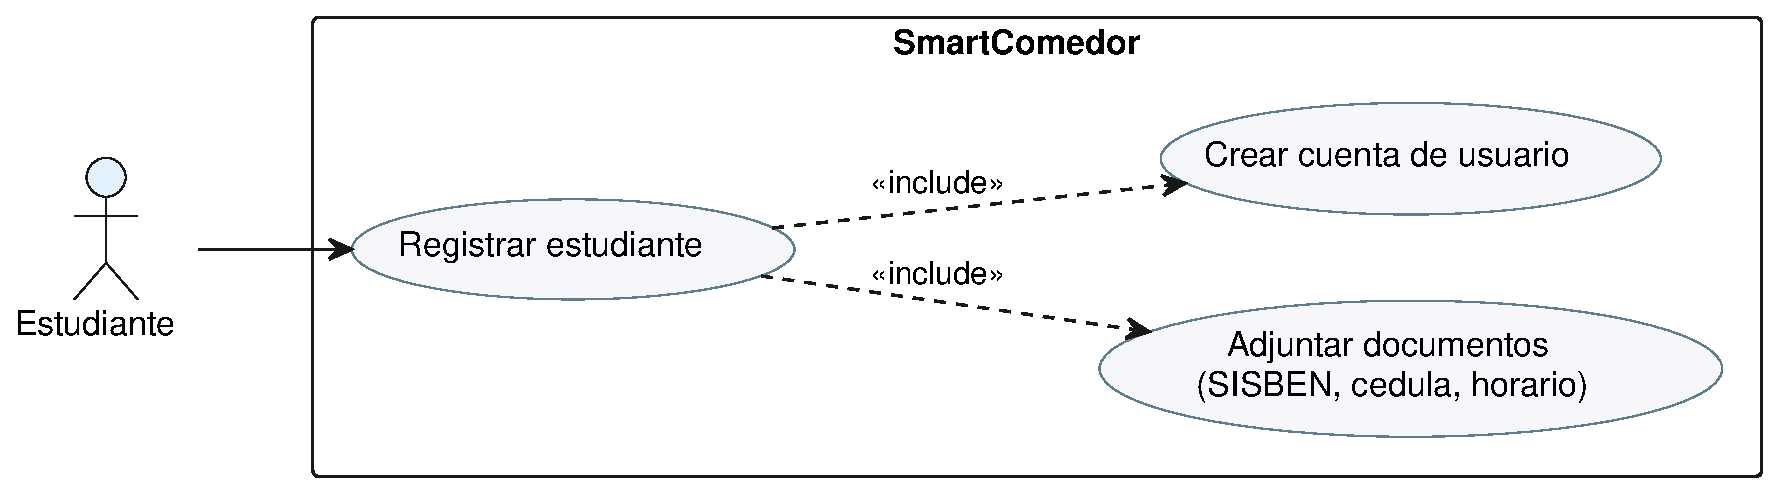
\includegraphics[width=\linewidth,height=0.30\textheight,keepaspectratio]{cu/cu01-uc.pdf}\caption{Diagrama de caso de uso --- CU-01}\end{figure}
\begin{figure}[H]\centering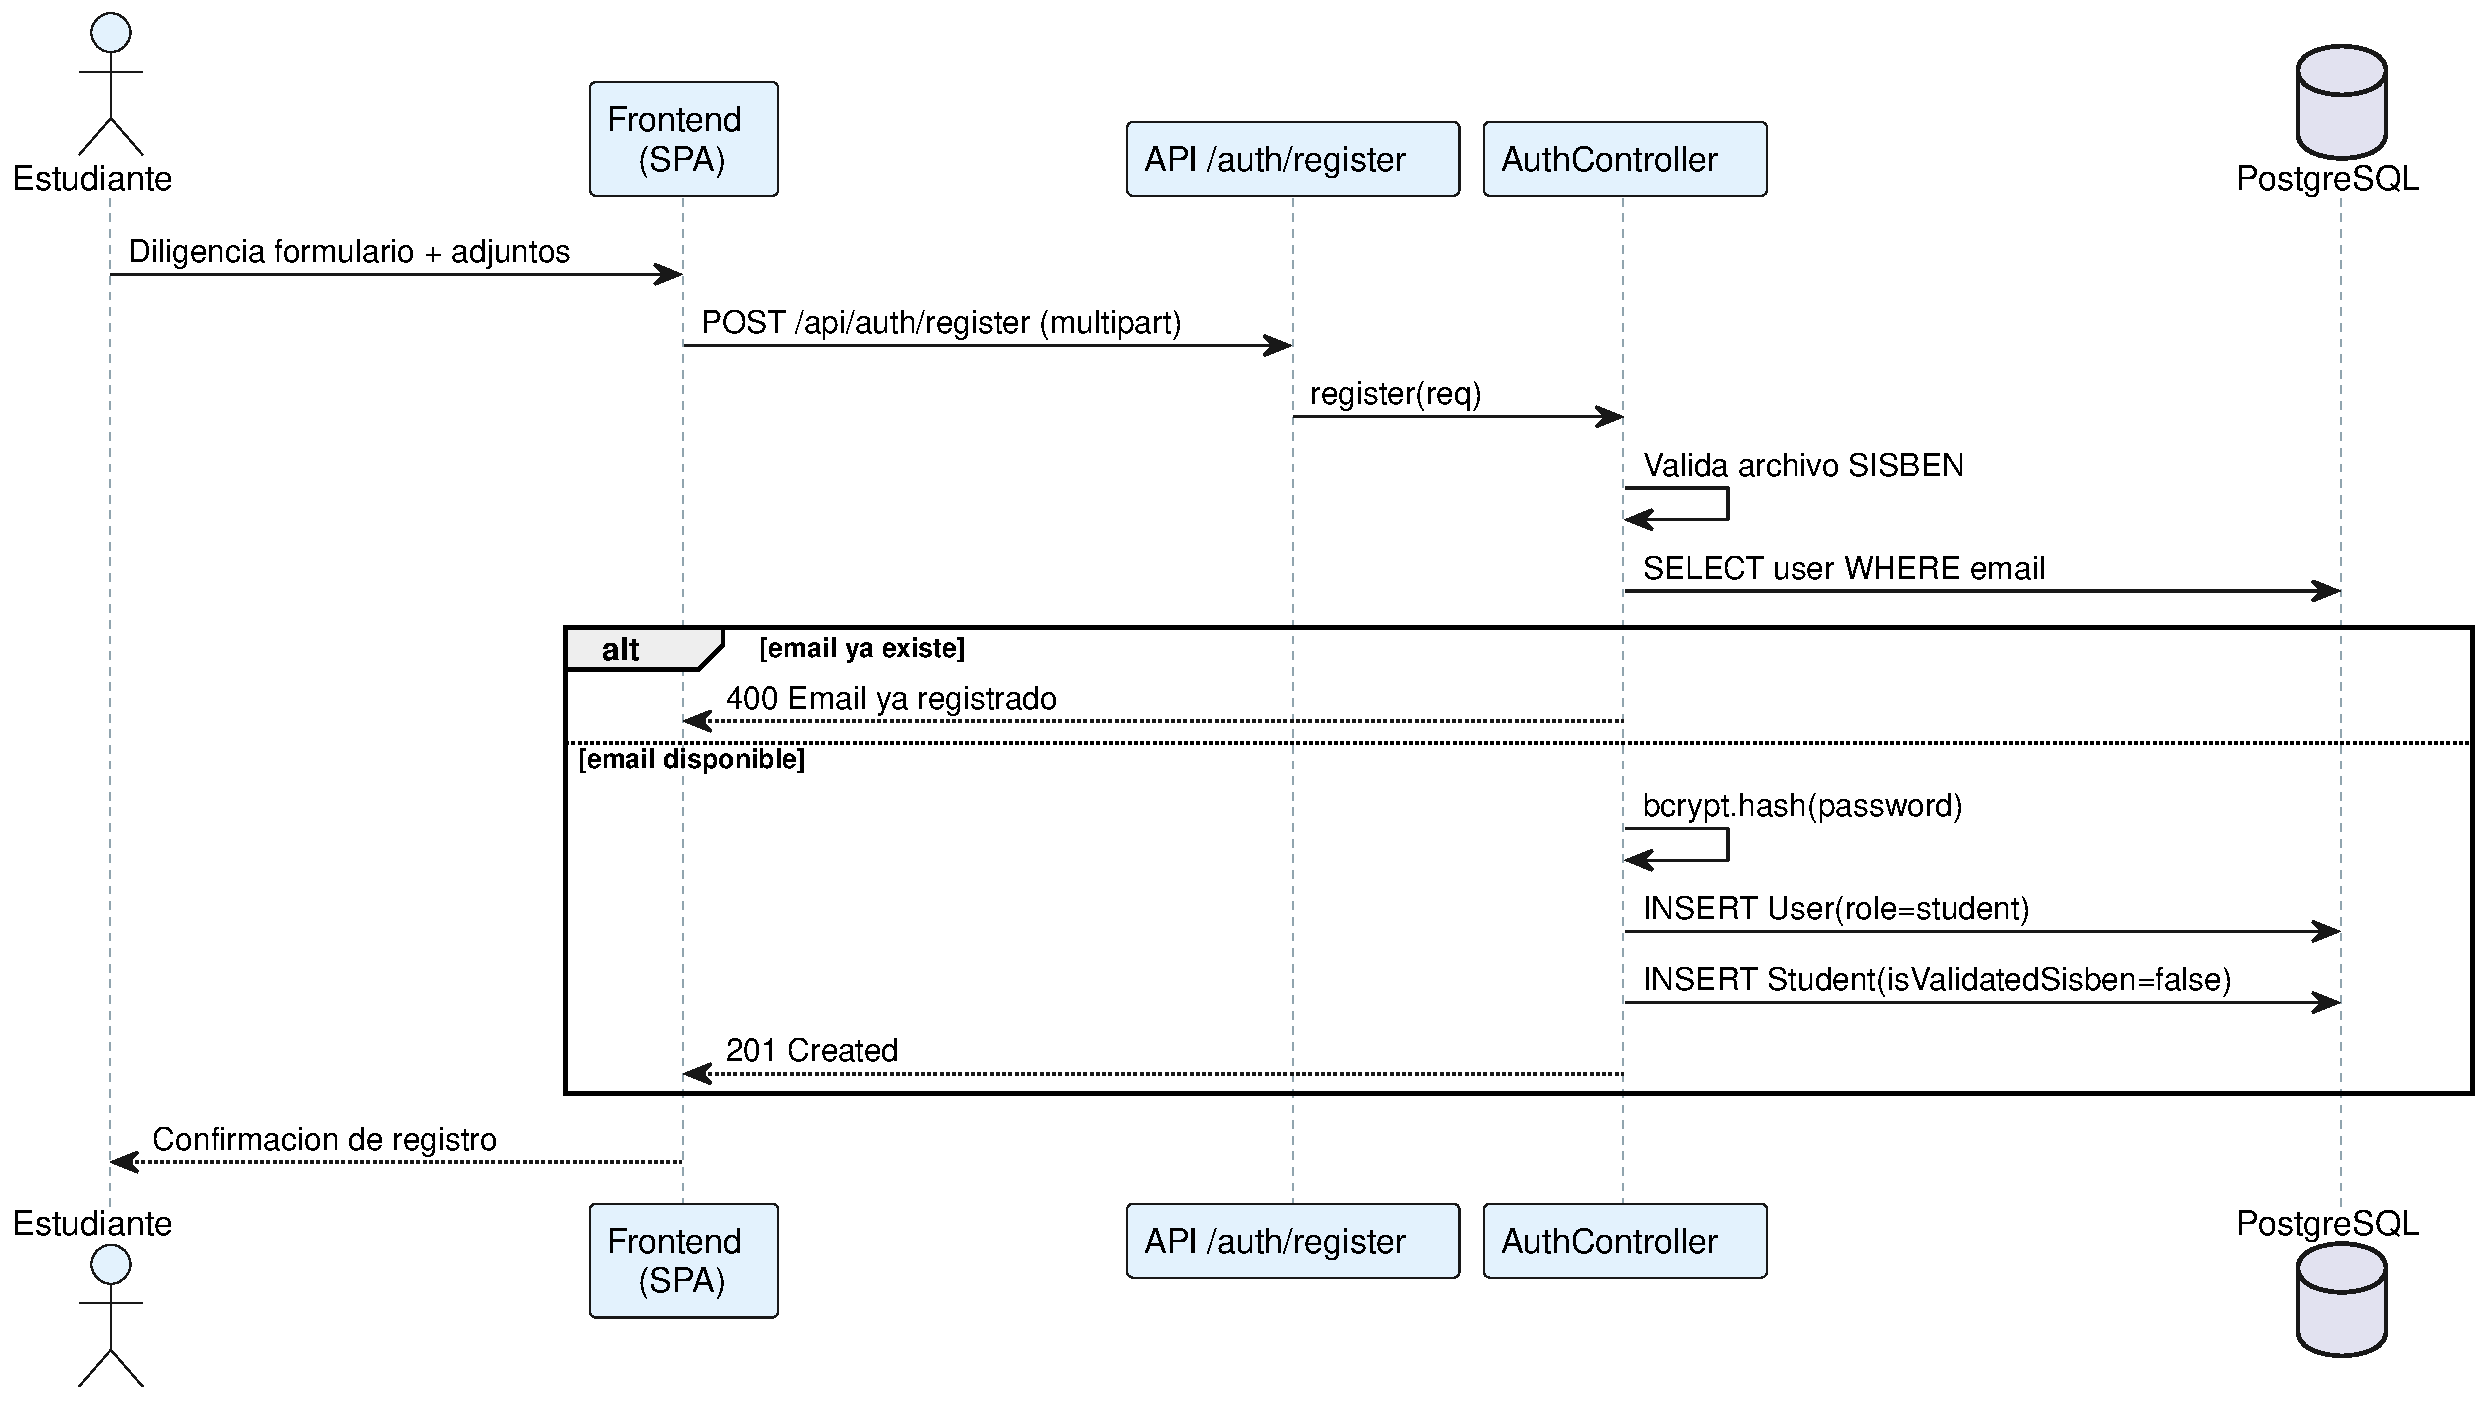
\includegraphics[width=\linewidth,height=0.42\textheight,keepaspectratio]{cu/cu01-seq.pdf}\caption{Diagrama de secuencia --- CU-01}\end{figure}
\begin{figure}[H]\centering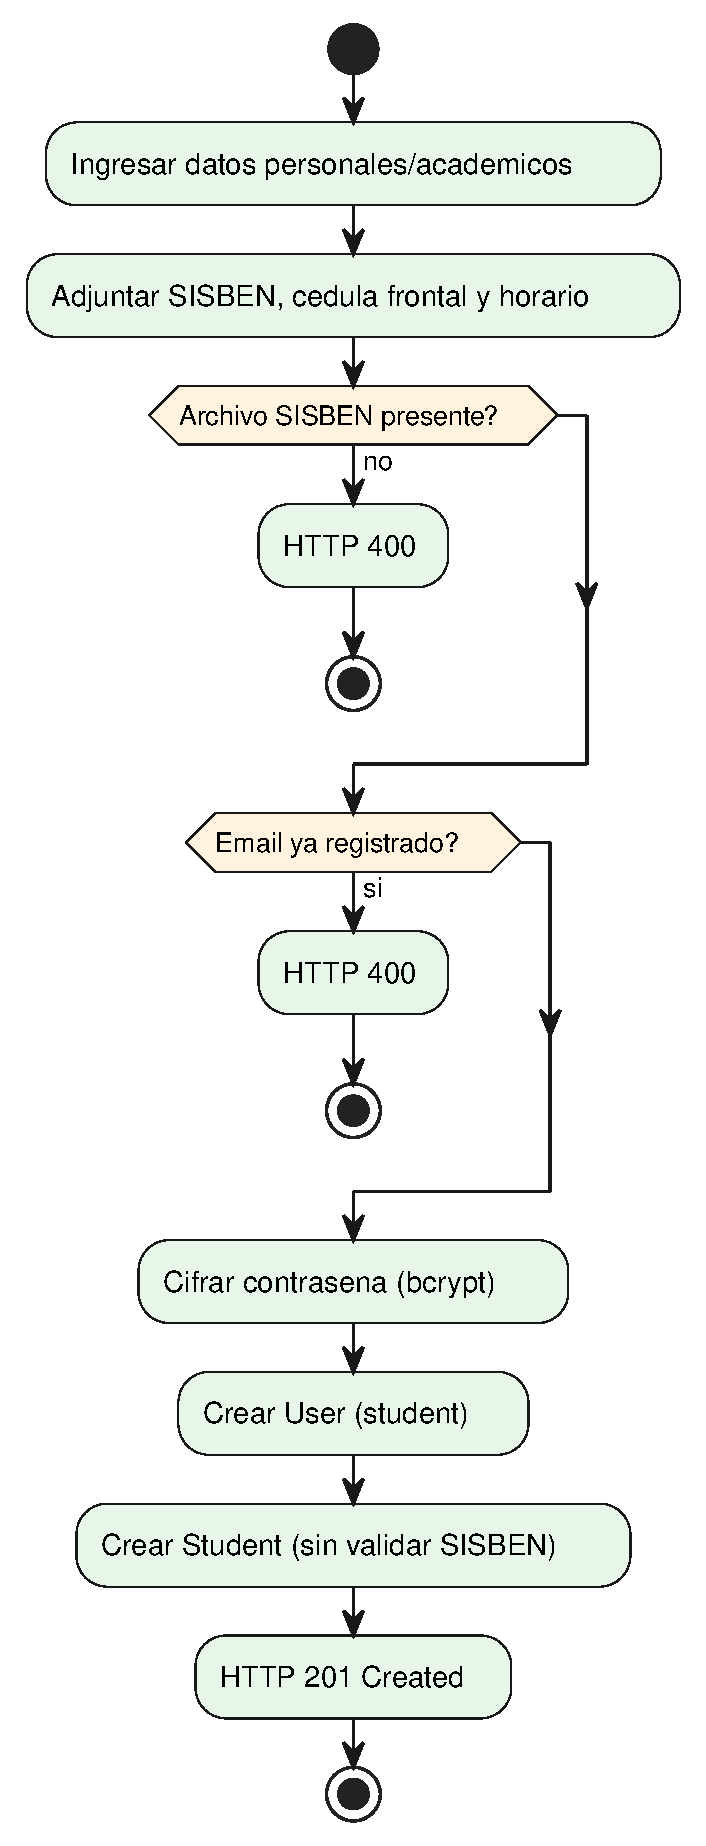
\includegraphics[width=\linewidth,height=0.46\textheight,keepaspectratio]{cu/cu01-act.pdf}\caption{Diagrama de actividades --- CU-01}\end{figure}

\subsection{CU-02 --- Iniciar sesion}

\noindent\textbf{Endpoint(s):} \texttt{POST /api/auth/login}\par\vspace{4pt}

\begin{table}[H]\centering\small
\caption{Ficha del caso de uso CU-02 --- Iniciar sesion}
\begin{tabularx}{\textwidth}{L{0.26\textwidth} X}
\toprule
\textbf{Campo} & \textbf{Descripcion} \\ \midrule
Objetivo del contexto & Permitir a un usuario autenticarse en el sistema mediante correo, contrasena y rol, obteniendo los tokens de acceso. \\ \midrule
Precondiciones & El usuario debe estar registrado y su cuenta activa. \\ \midrule
Condicion de exito & Se emiten los tokens de acceso y refresco; el usuario accede segun su rol. \\ \midrule
Condicion de fracaso & Acceso denegado por credenciales, estado o rol invalidos. \\ \midrule
Actores principales & Usuario (estudiante, supervisor, administrador, auditor) \\ \midrule
Actores secundarios & Servicio de autenticacion JWT \\
\bottomrule\end{tabularx}\end{table}
\begin{table}[H]\centering\small
\caption{Flujo principal de CU-02}
\begin{tabularx}{\textwidth}{C{0.10\textwidth} X}
\toprule \textbf{Paso} & \textbf{Accion} \\ \midrule
1 & El usuario ingresa correo, contrasena y rol. \\
2 & El sistema valida que los campos esten completos. \\
3 & El sistema busca al usuario por correo. \\
4 & El sistema verifica la contrasena con bcrypt.compare. \\
5 & El sistema valida que la cuenta este activa, autorizada y que el rol coincida. \\
6 & El sistema emite access y refresh token y responde 200. \\
\bottomrule\end{tabularx}\end{table}
\begin{table}[H]\centering\small
\caption{Extensiones (flujos alternativos) de CU-02}
\begin{tabularx}{\textwidth}{C{0.10\textwidth} X}
\toprule \textbf{Paso} & \textbf{Accion} \\ \midrule
2.1 & Campos faltantes $\rightarrow$ HTTP 400. \\
3.1 & Usuario inexistente $\rightarrow$ HTTP 401. \\
4.1 & Contrasena incorrecta $\rightarrow$ HTTP 401. \\
5.1 & Cuenta inactiva $\rightarrow$ 401; rol no coincide o no autorizado $\rightarrow$ 403. \\
\bottomrule\end{tabularx}\end{table}
\begin{figure}[H]\centering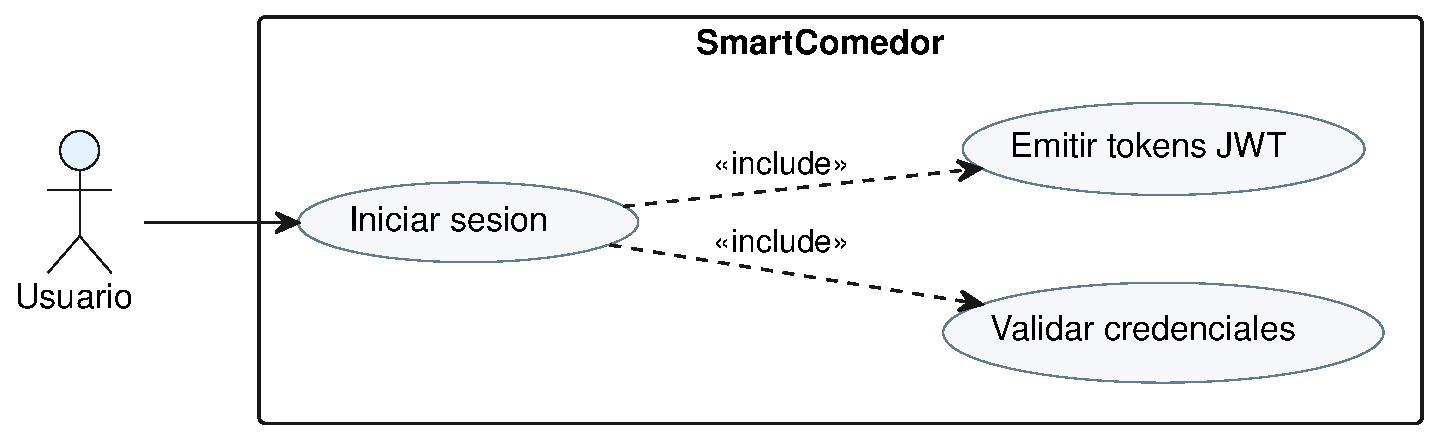
\includegraphics[width=\linewidth,height=0.30\textheight,keepaspectratio]{cu/cu02-uc.pdf}\caption{Diagrama de caso de uso --- CU-02}\end{figure}
\begin{figure}[H]\centering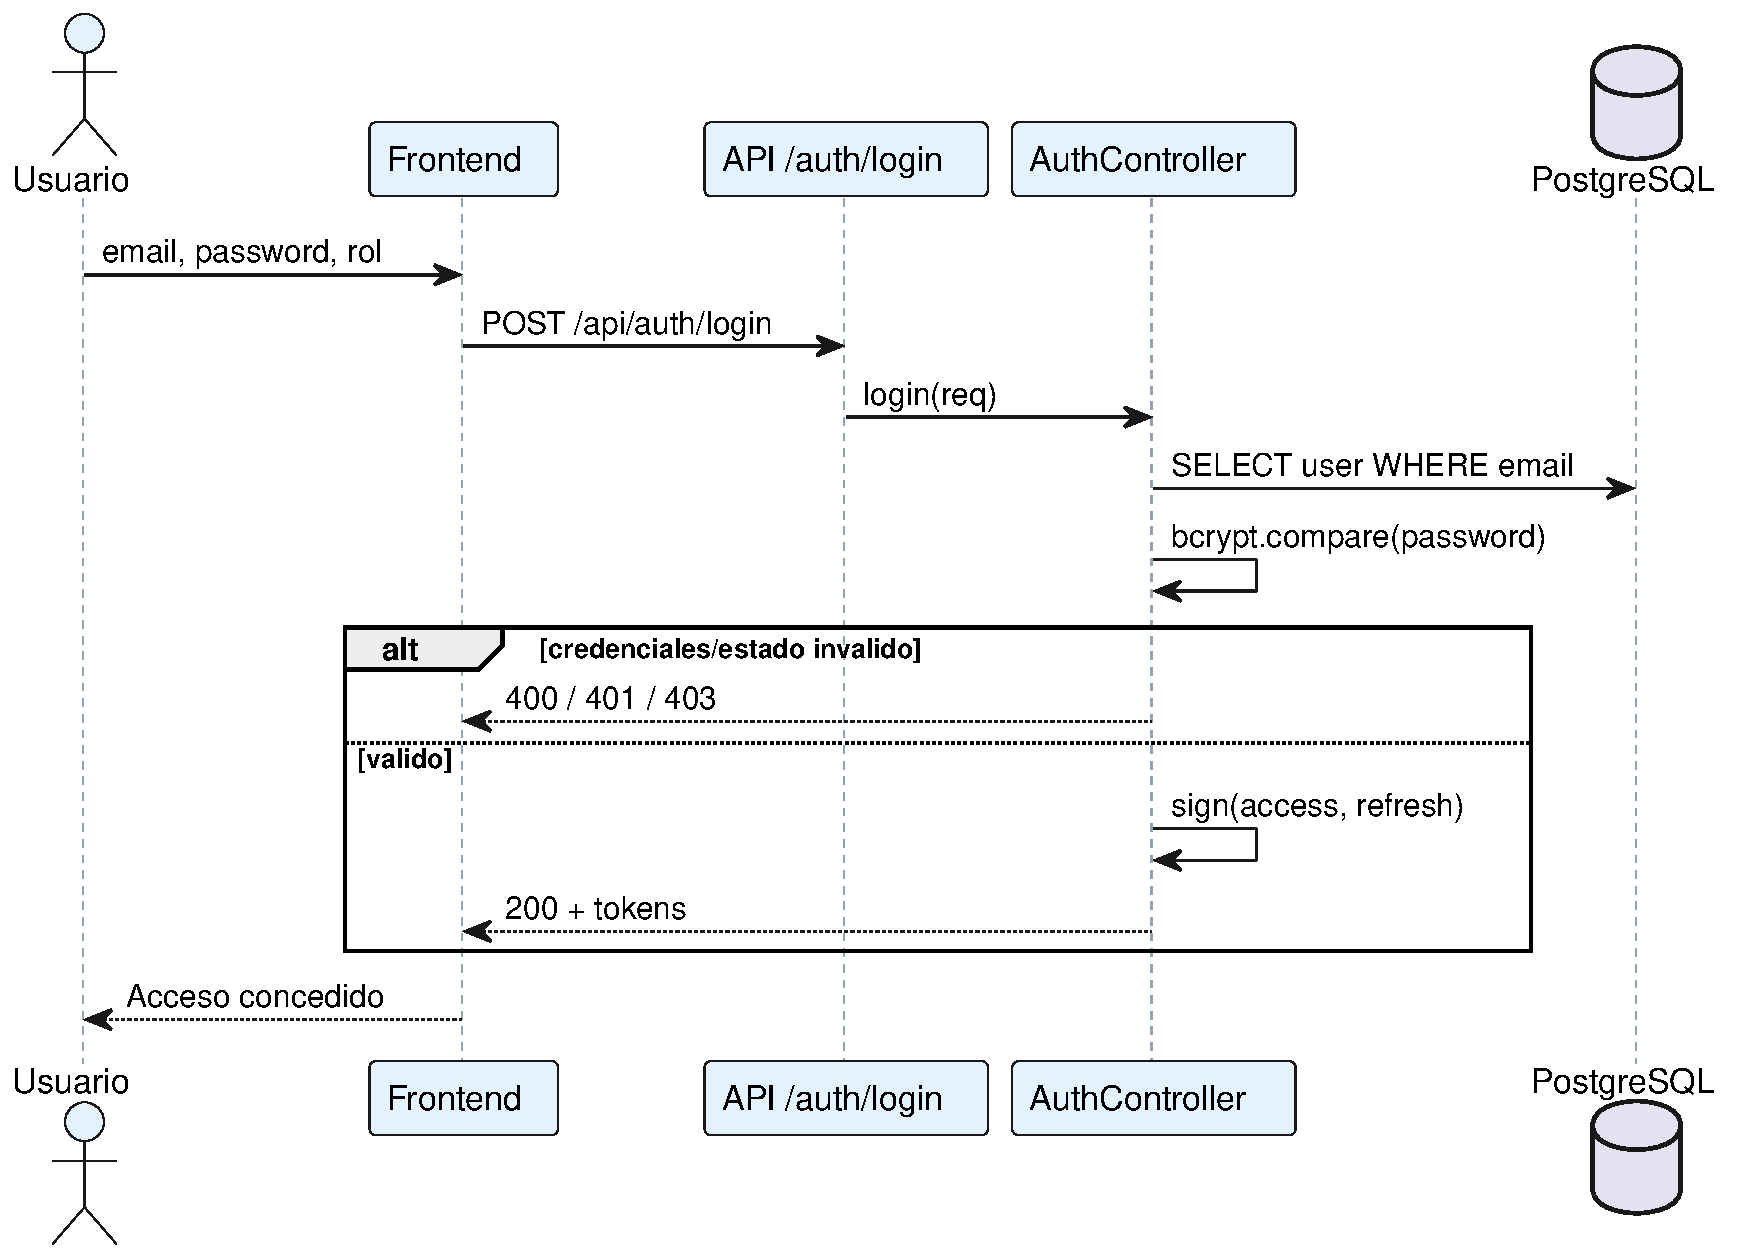
\includegraphics[width=\linewidth,height=0.42\textheight,keepaspectratio]{cu/cu02-seq.pdf}\caption{Diagrama de secuencia --- CU-02}\end{figure}
\begin{figure}[H]\centering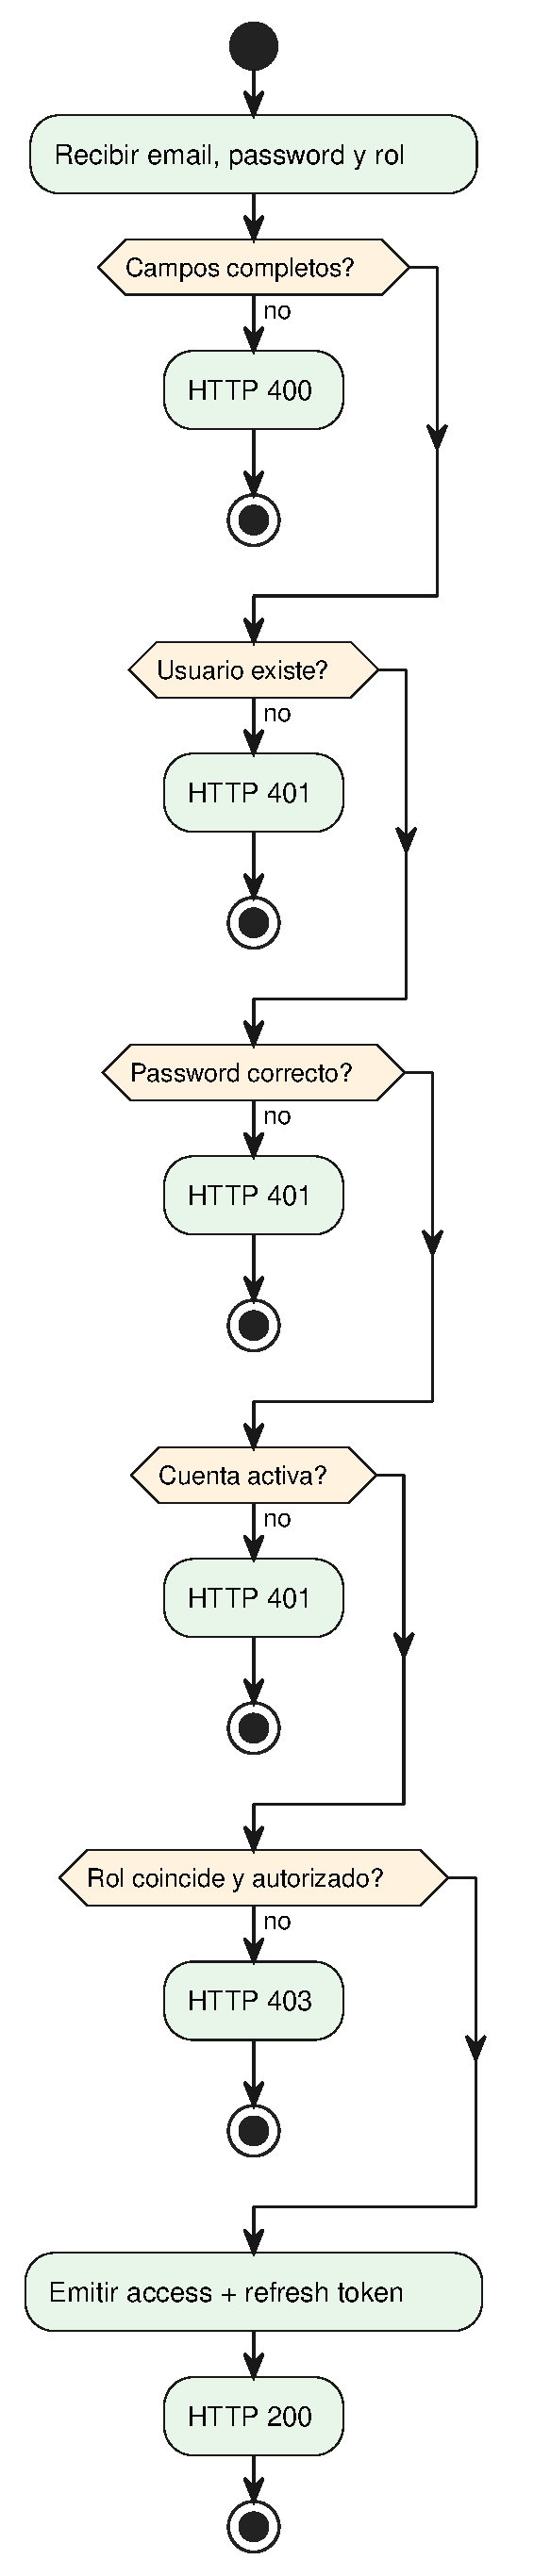
\includegraphics[width=\linewidth,height=0.46\textheight,keepaspectratio]{cu/cu02-act.pdf}\caption{Diagrama de actividades --- CU-02}\end{figure}

\subsection{CU-03 --- Recuperar y restablecer contrasena}

\noindent\textbf{Endpoint(s):} \texttt{POST /api/auth/forgot-password, POST /api/auth/reset-password}\par\vspace{4pt}

\begin{table}[H]\centering\small
\caption{Ficha del caso de uso CU-03 --- Recuperar y restablecer contrasena}
\begin{tabularx}{\textwidth}{L{0.26\textwidth} X}
\toprule
\textbf{Campo} & \textbf{Descripcion} \\ \midrule
Objetivo del contexto & Permitir al usuario recuperar el acceso cuando olvida su contrasena, mediante un enlace con token enviado por correo. \\ \midrule
Precondiciones & El usuario debe tener un correo registrado. \\ \midrule
Condicion de exito & La contrasena se actualiza y el usuario puede iniciar sesion. \\ \midrule
Condicion de fracaso & El token es invalido o esta expirado. \\ \midrule
Actores principales & Usuario \\ \midrule
Actores secundarios & Servicio de correo (Nodemailer) \\
\bottomrule\end{tabularx}\end{table}
\begin{table}[H]\centering\small
\caption{Flujo principal de CU-03}
\begin{tabularx}{\textwidth}{C{0.10\textwidth} X}
\toprule \textbf{Paso} & \textbf{Accion} \\ \midrule
1 & El usuario solicita recuperacion indicando su correo. \\
2 & El sistema genera un token con expiracion y lo almacena. \\
3 & El sistema envia un correo con el enlace (mensaje generico). \\
4 & El usuario abre el enlace e ingresa la nueva contrasena. \\
5 & El sistema valida el token y actualiza la contrasena cifrada. \\
6 & El sistema responde 200. \\
\bottomrule\end{tabularx}\end{table}
\begin{table}[H]\centering\small
\caption{Extensiones (flujos alternativos) de CU-03}
\begin{tabularx}{\textwidth}{C{0.10\textwidth} X}
\toprule \textbf{Paso} & \textbf{Accion} \\ \midrule
3.1 & Por seguridad, el mensaje no revela si el correo existe. \\
5.1 & Token invalido o expirado $\rightarrow$ HTTP 400. \\
\bottomrule\end{tabularx}\end{table}
\begin{figure}[H]\centering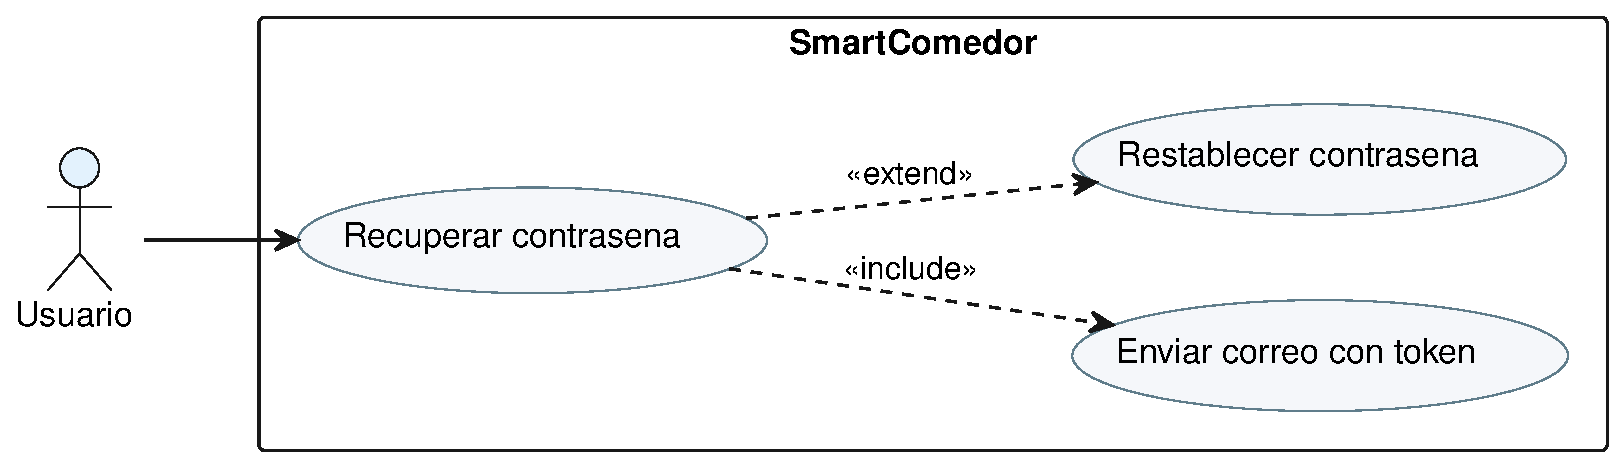
\includegraphics[width=\linewidth,height=0.30\textheight,keepaspectratio]{cu/cu03-uc.pdf}\caption{Diagrama de caso de uso --- CU-03}\end{figure}
\begin{figure}[H]\centering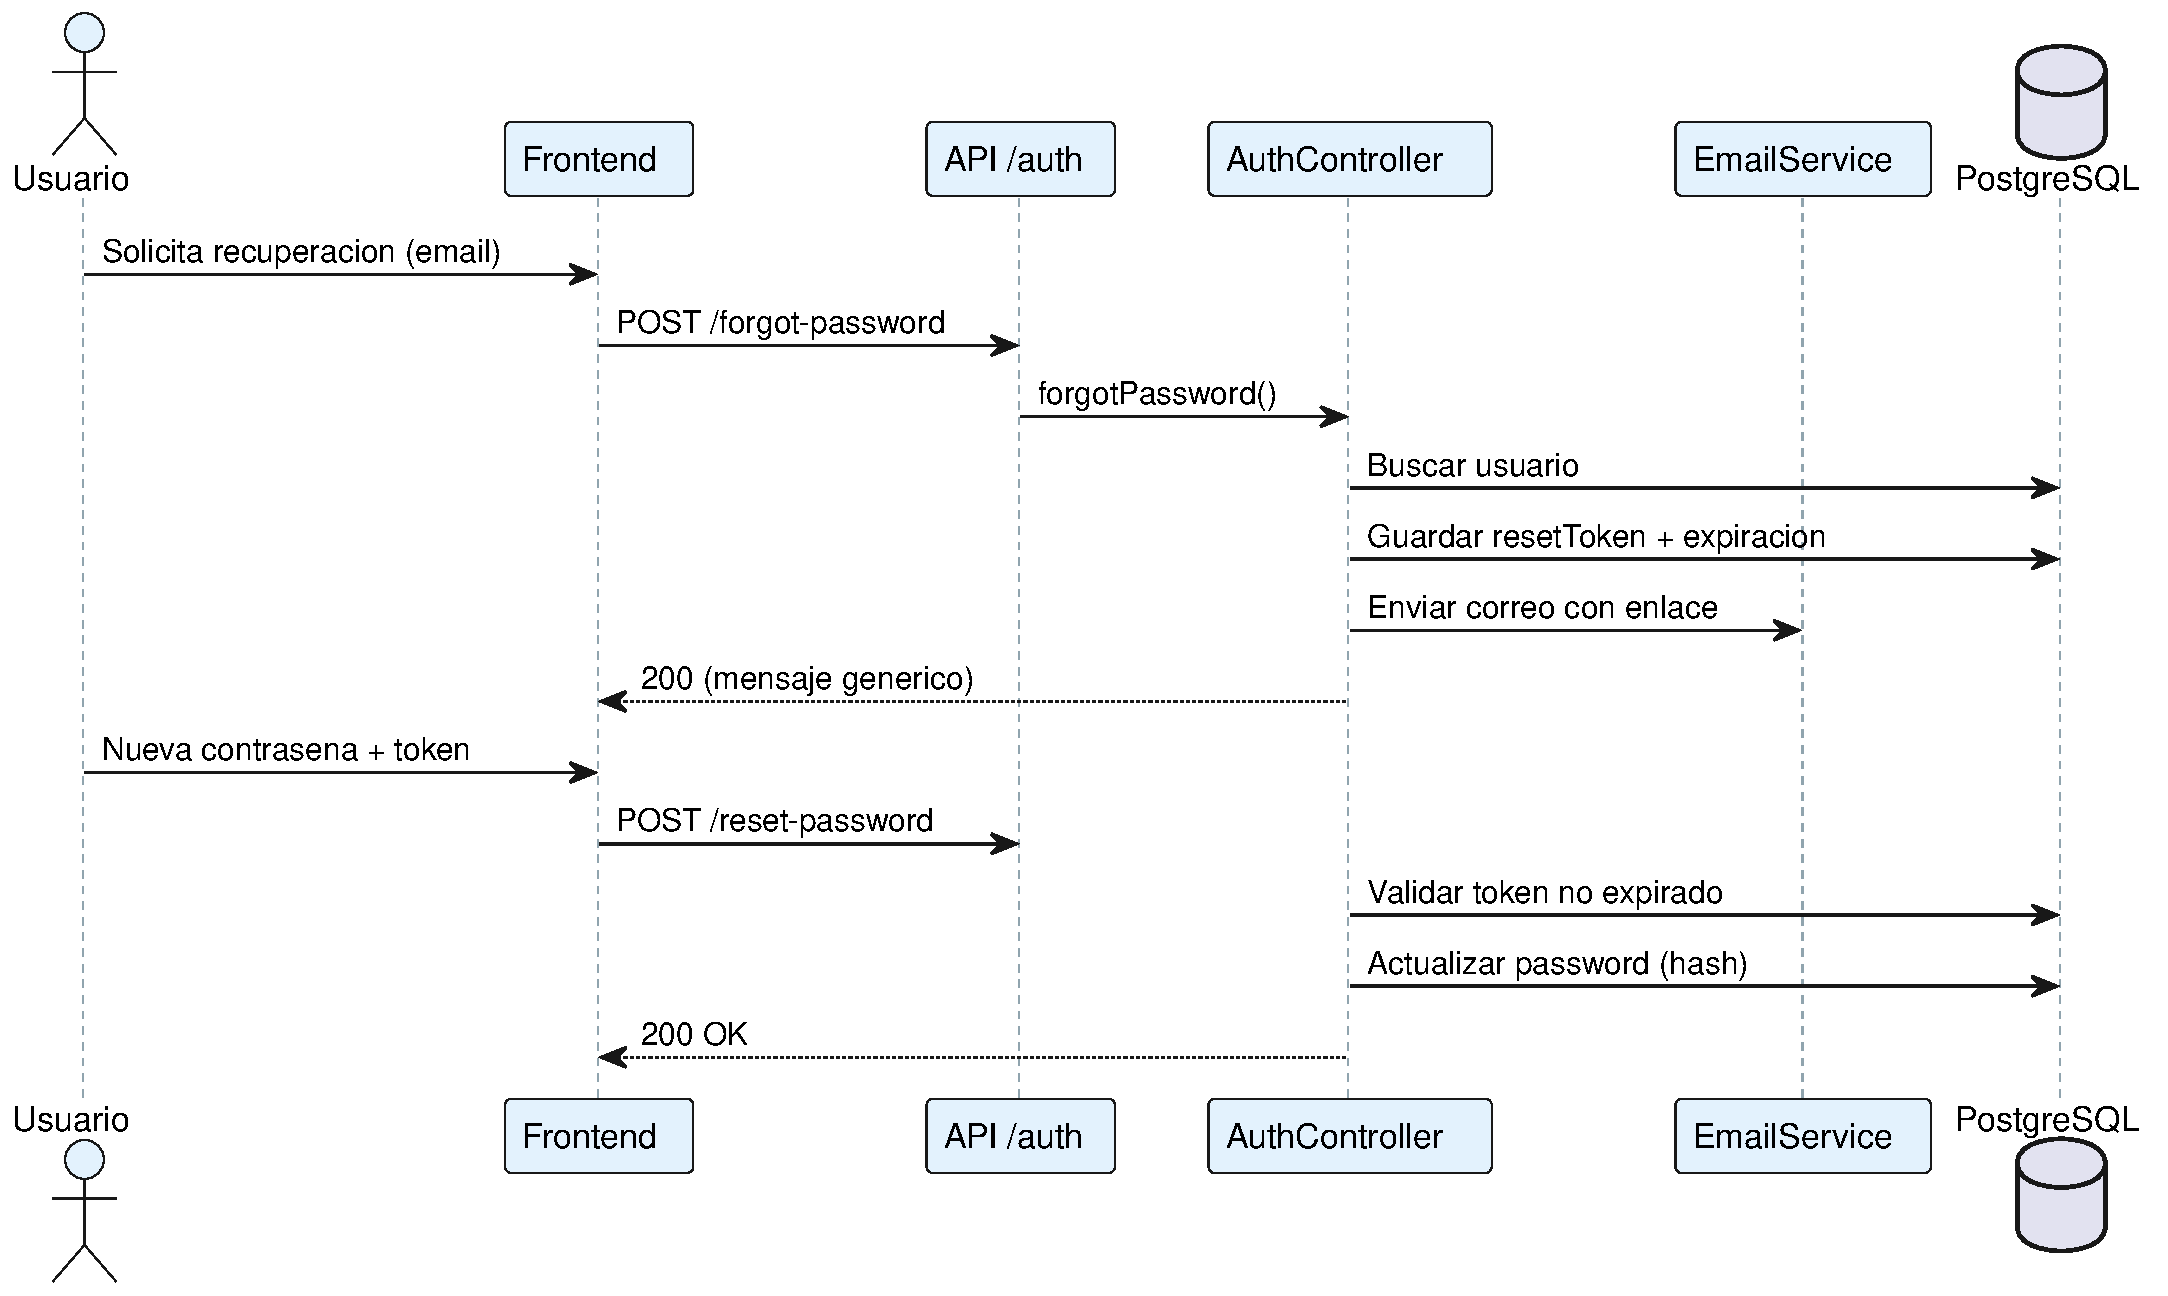
\includegraphics[width=\linewidth,height=0.42\textheight,keepaspectratio]{cu/cu03-seq.pdf}\caption{Diagrama de secuencia --- CU-03}\end{figure}
\begin{figure}[H]\centering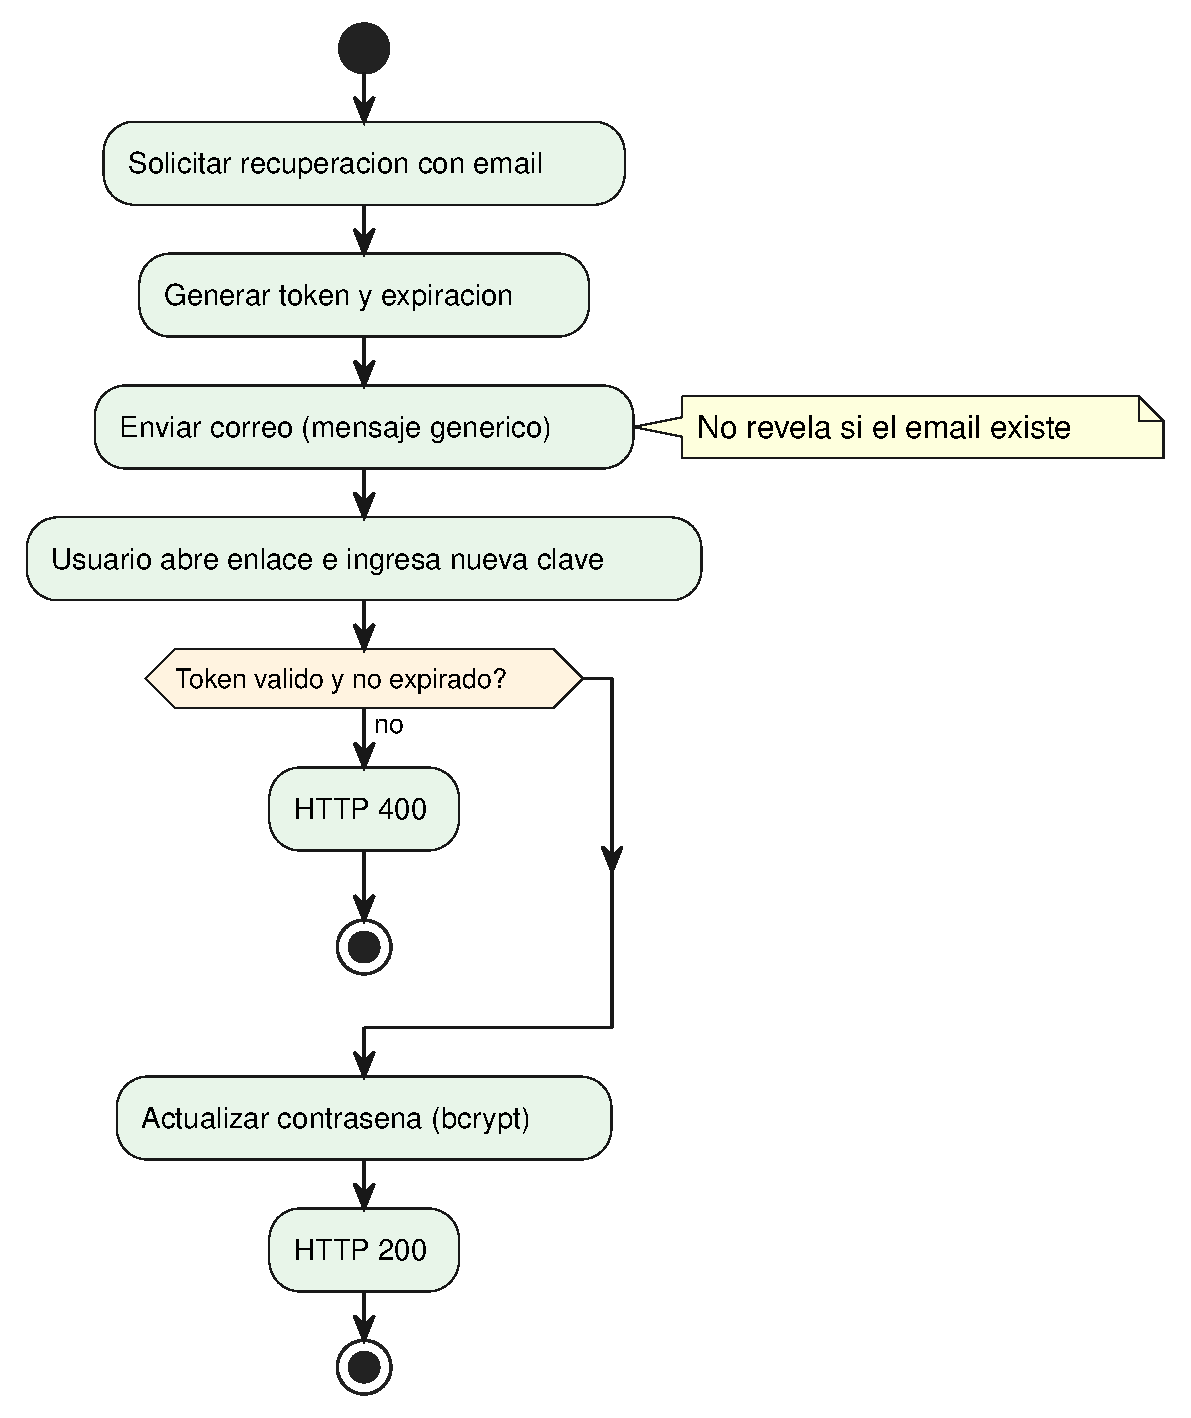
\includegraphics[width=\linewidth,height=0.46\textheight,keepaspectratio]{cu/cu03-act.pdf}\caption{Diagrama de actividades --- CU-03}\end{figure}

\subsection{CU-04 --- Configurar y verificar 2FA}

\noindent\textbf{Endpoint(s):} \texttt{POST /api/auth/setup-2fa, POST /api/auth/verify-2fa}\par\vspace{4pt}

\begin{table}[H]\centering\small
\caption{Ficha del caso de uso CU-04 --- Configurar y verificar 2FA}
\begin{tabularx}{\textwidth}{L{0.26\textwidth} X}
\toprule
\textbf{Campo} & \textbf{Descripcion} \\ \midrule
Objetivo del contexto & Permitir al estudiante activar un segundo factor de autenticacion (TOTP) para reforzar la seguridad de su cuenta. \\ \midrule
Precondiciones & El usuario debe estar autenticado. \\ \midrule
Condicion de exito & El segundo factor queda activo y se exige en posteriores inicios de sesion. \\ \midrule
Condicion de fracaso & El codigo TOTP ingresado es invalido. \\ \midrule
Actores principales & Estudiante \\ \midrule
Actores secundarios & Aplicacion autenticadora (TOTP) \\
\bottomrule\end{tabularx}\end{table}
\begin{table}[H]\centering\small
\caption{Flujo principal de CU-04}
\begin{tabularx}{\textwidth}{C{0.10\textwidth} X}
\toprule \textbf{Paso} & \textbf{Accion} \\ \midrule
1 & El usuario solicita activar 2FA. \\
2 & El sistema genera un secreto TOTP y un codigo QR. \\
3 & El usuario escanea el QR en su aplicacion autenticadora. \\
4 & El usuario ingresa el codigo de 6 digitos. \\
5 & El sistema verifica el codigo con speakeasy y activa el 2FA. \\
6 & El sistema responde 200. \\
\bottomrule\end{tabularx}\end{table}
\begin{table}[H]\centering\small
\caption{Extensiones (flujos alternativos) de CU-04}
\begin{tabularx}{\textwidth}{C{0.10\textwidth} X}
\toprule \textbf{Paso} & \textbf{Accion} \\ \midrule
5.1 & Codigo TOTP invalido $\rightarrow$ HTTP 400. \\
\bottomrule\end{tabularx}\end{table}
\begin{figure}[H]\centering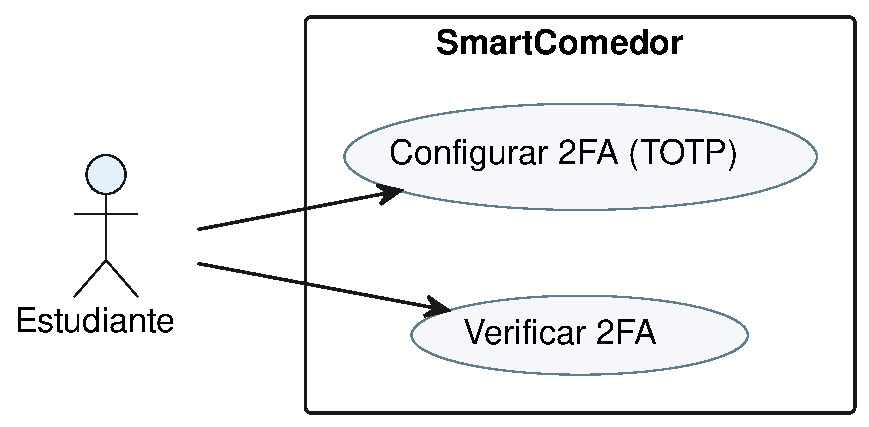
\includegraphics[width=\linewidth,height=0.30\textheight,keepaspectratio]{cu/cu04-uc.pdf}\caption{Diagrama de caso de uso --- CU-04}\end{figure}
\begin{figure}[H]\centering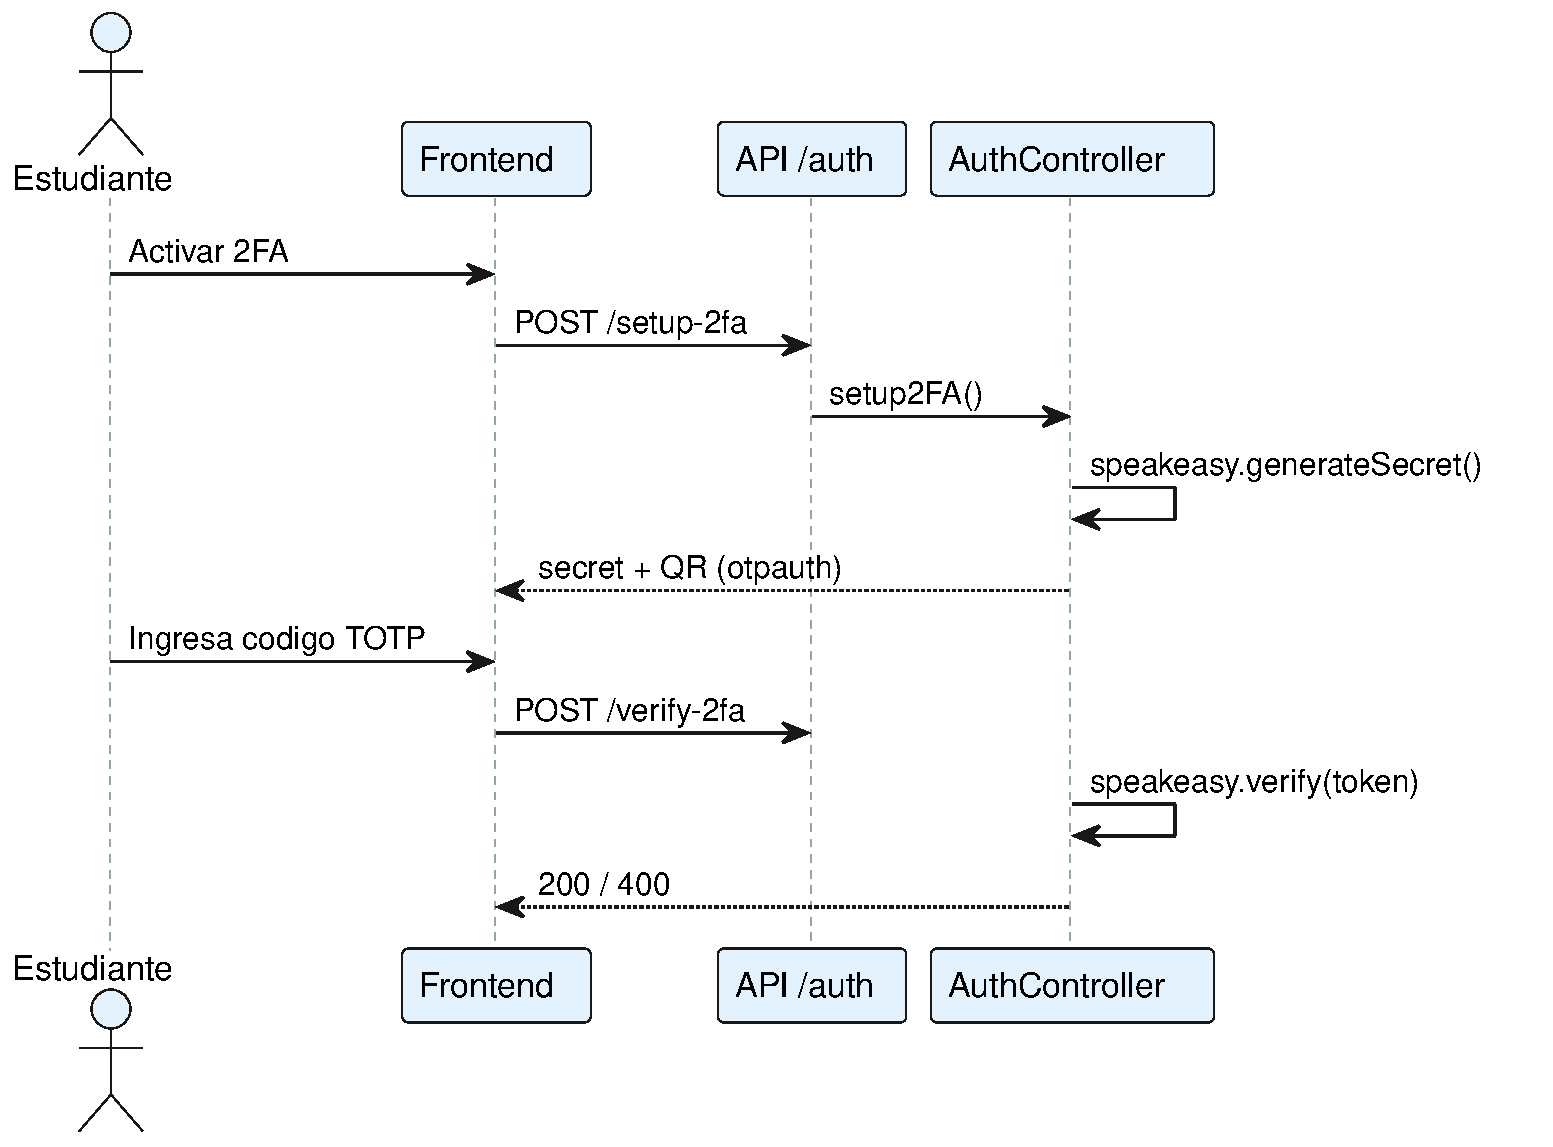
\includegraphics[width=\linewidth,height=0.42\textheight,keepaspectratio]{cu/cu04-seq.pdf}\caption{Diagrama de secuencia --- CU-04}\end{figure}
\begin{figure}[H]\centering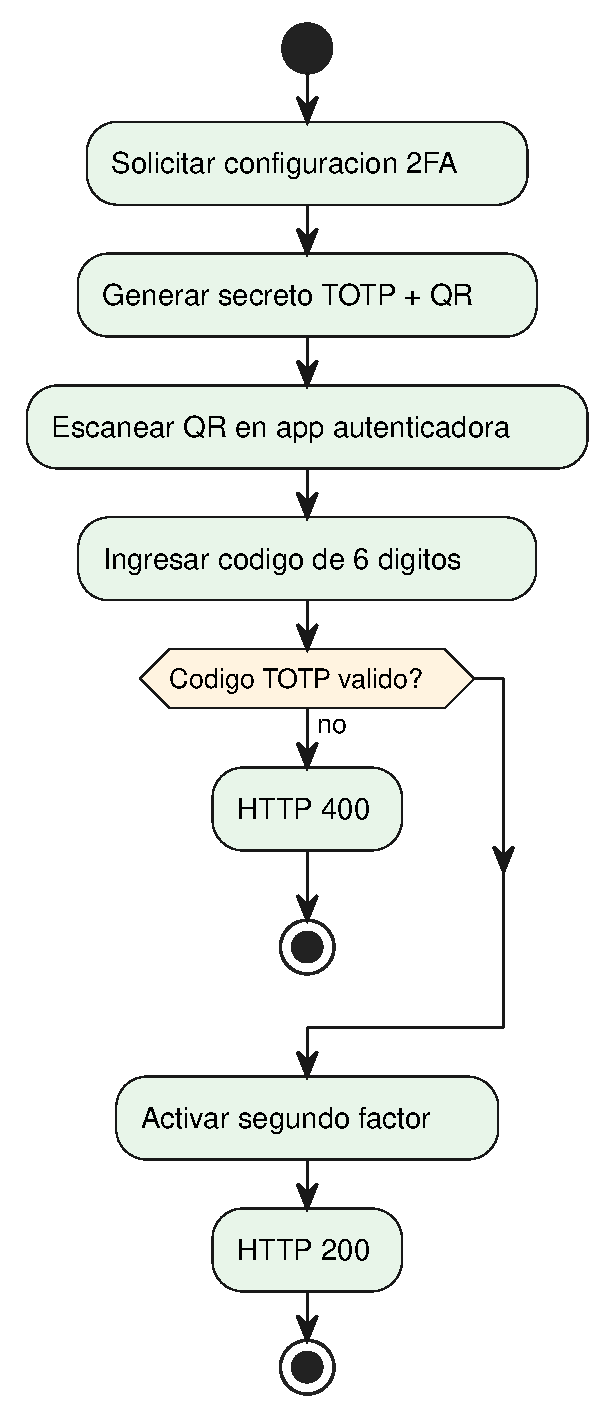
\includegraphics[width=\linewidth,height=0.46\textheight,keepaspectratio]{cu/cu04-act.pdf}\caption{Diagrama de actividades --- CU-04}\end{figure}

\subsection{CU-05 --- Gestionar estudiantes (CRUD)}

\noindent\textbf{Endpoint(s):} \texttt{GET/POST/PUT/DELETE /api/students}\par\vspace{4pt}

\begin{table}[H]\centering\small
\caption{Ficha del caso de uso CU-05 --- Gestionar estudiantes (CRUD)}
\begin{tabularx}{\textwidth}{L{0.26\textwidth} X}
\toprule
\textbf{Campo} & \textbf{Descripcion} \\ \midrule
Objetivo del contexto & Permitir al administrador listar, consultar, crear, actualizar y deshabilitar estudiantes del sistema. \\ \midrule
Precondiciones & El administrador debe estar autenticado con rol admin. \\ \midrule
Condicion de exito & La operacion solicitada se refleja en la base de datos. \\ \midrule
Condicion de fracaso & Datos invalidos o estudiante inexistente. \\ \midrule
Actores principales & Administrador \\ \midrule
Actores secundarios & Base de datos \\
\bottomrule\end{tabularx}\end{table}
\begin{table}[H]\centering\small
\caption{Flujo principal de CU-05}
\begin{tabularx}{\textwidth}{C{0.10\textwidth} X}
\toprule \textbf{Paso} & \textbf{Accion} \\ \midrule
1 & El administrador abre la gestion de estudiantes. \\
2 & El sistema lista los estudiantes con paginacion y filtros. \\
3 & El administrador selecciona crear, editar o deshabilitar. \\
4 & El sistema valida los datos y ejecuta la operacion. \\
5 & El sistema responde con el recurso afectado. \\
\bottomrule\end{tabularx}\end{table}
\begin{table}[H]\centering\small
\caption{Extensiones (flujos alternativos) de CU-05}
\begin{tabularx}{\textwidth}{C{0.10\textwidth} X}
\toprule \textbf{Paso} & \textbf{Accion} \\ \midrule
4.1 & Datos invalidos $\rightarrow$ HTTP 400. \\
4.2 & Estudiante inexistente $\rightarrow$ HTTP 404. \\
\bottomrule\end{tabularx}\end{table}
\begin{figure}[H]\centering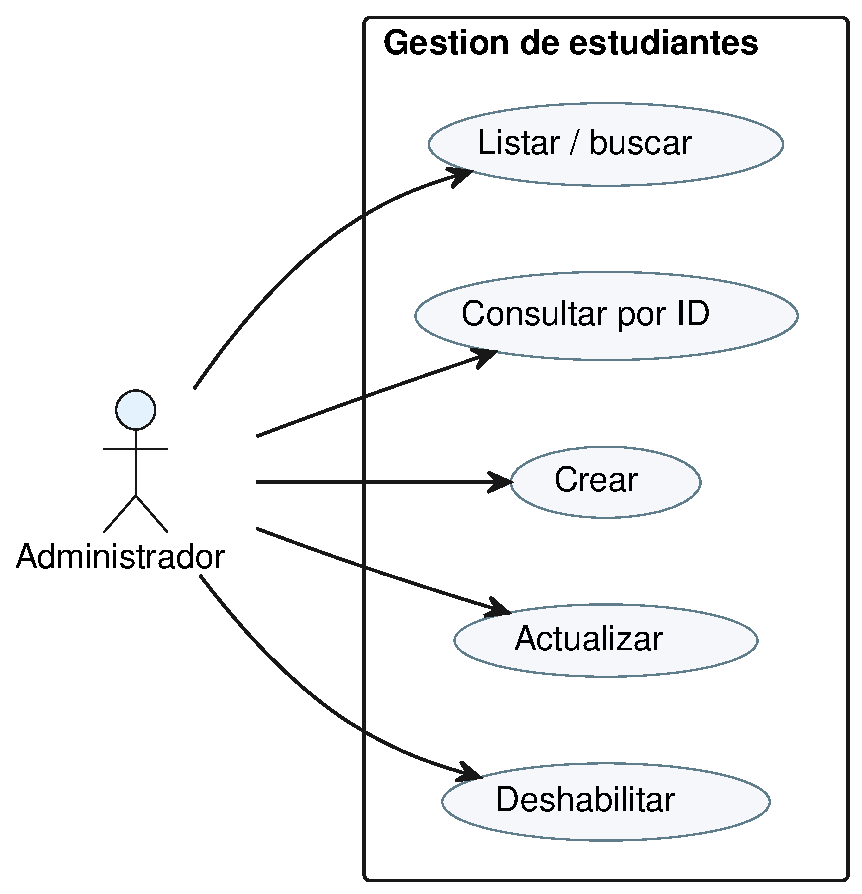
\includegraphics[width=\linewidth,height=0.30\textheight,keepaspectratio]{cu/cu05-uc.pdf}\caption{Diagrama de caso de uso --- CU-05}\end{figure}
\begin{figure}[H]\centering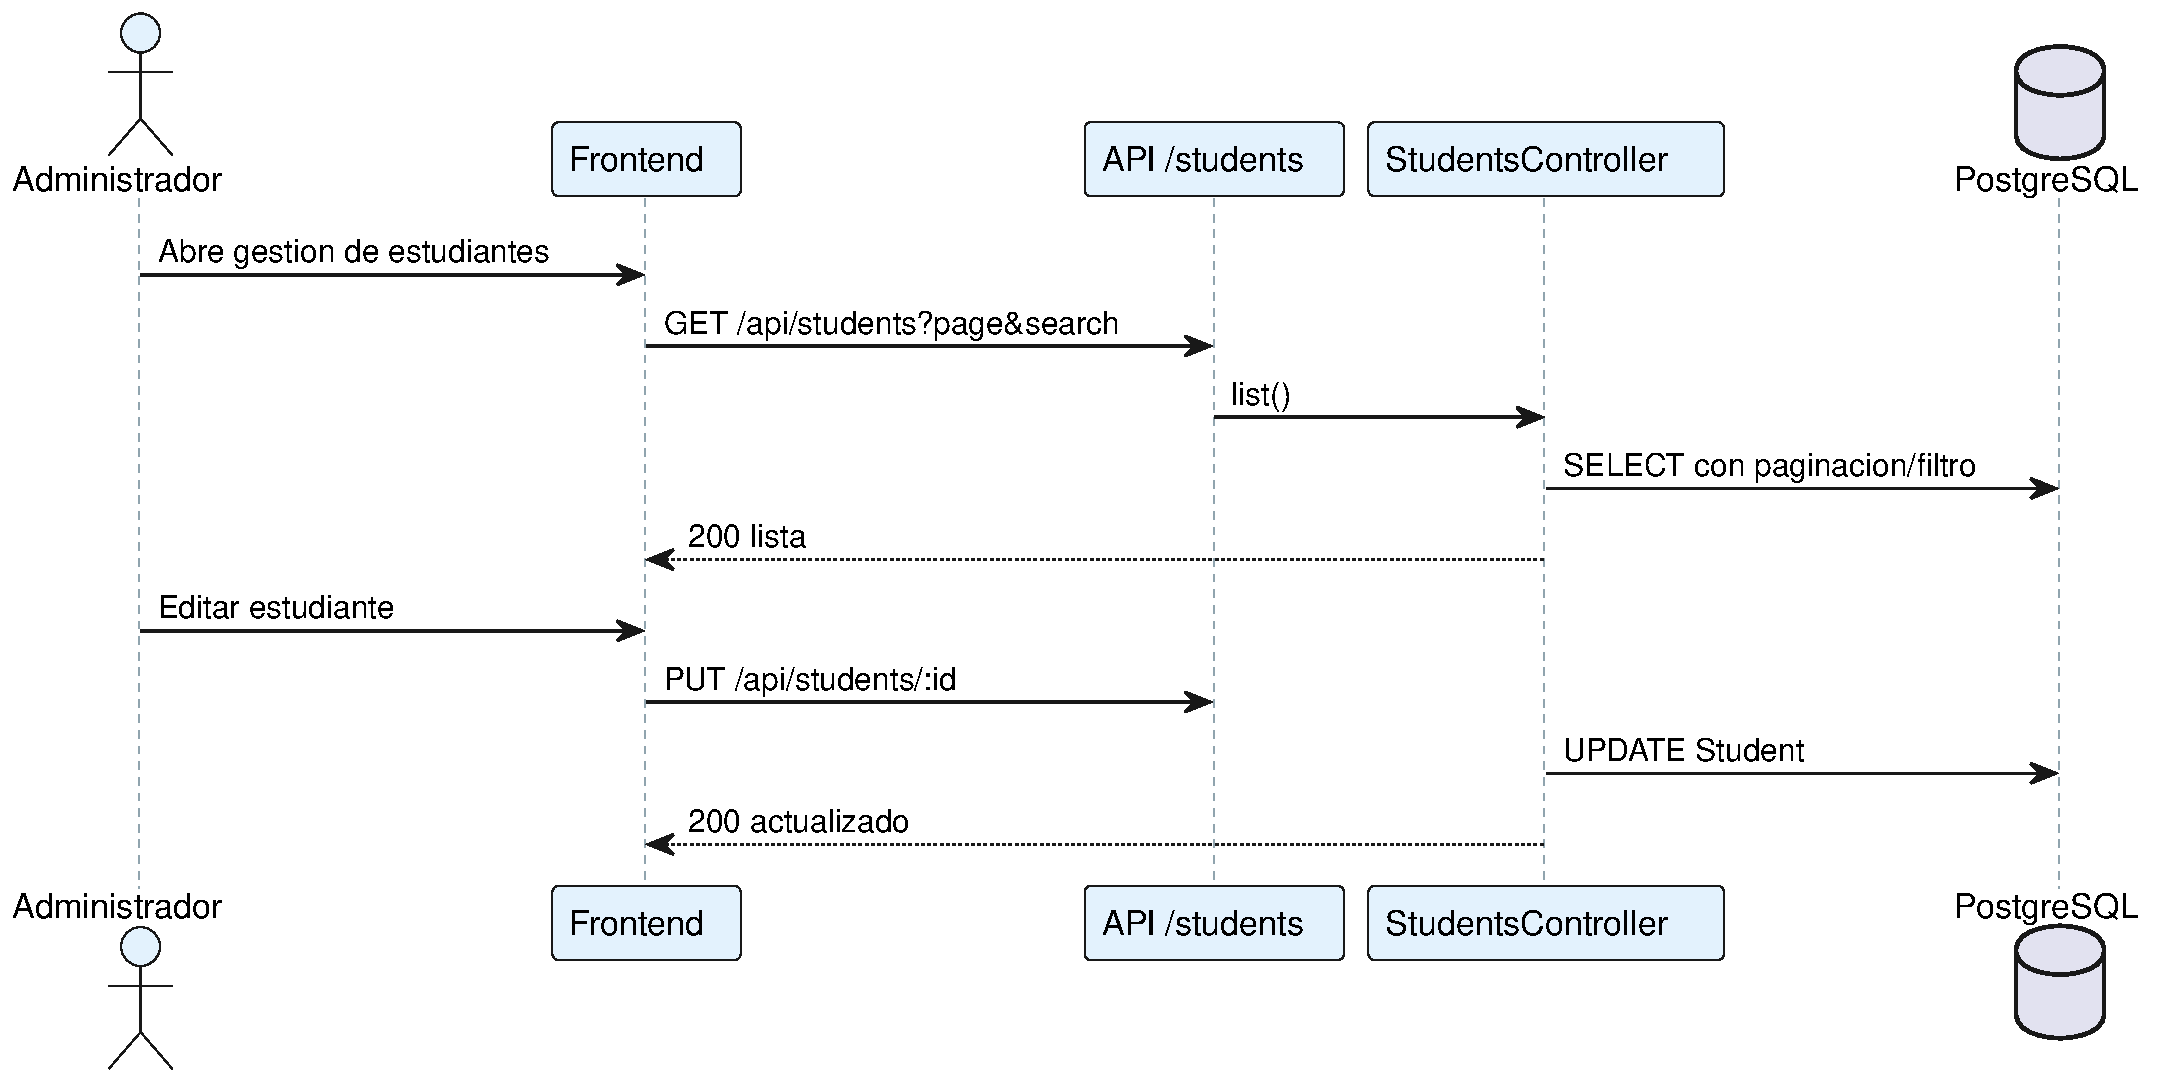
\includegraphics[width=\linewidth,height=0.42\textheight,keepaspectratio]{cu/cu05-seq.pdf}\caption{Diagrama de secuencia --- CU-05}\end{figure}
\begin{figure}[H]\centering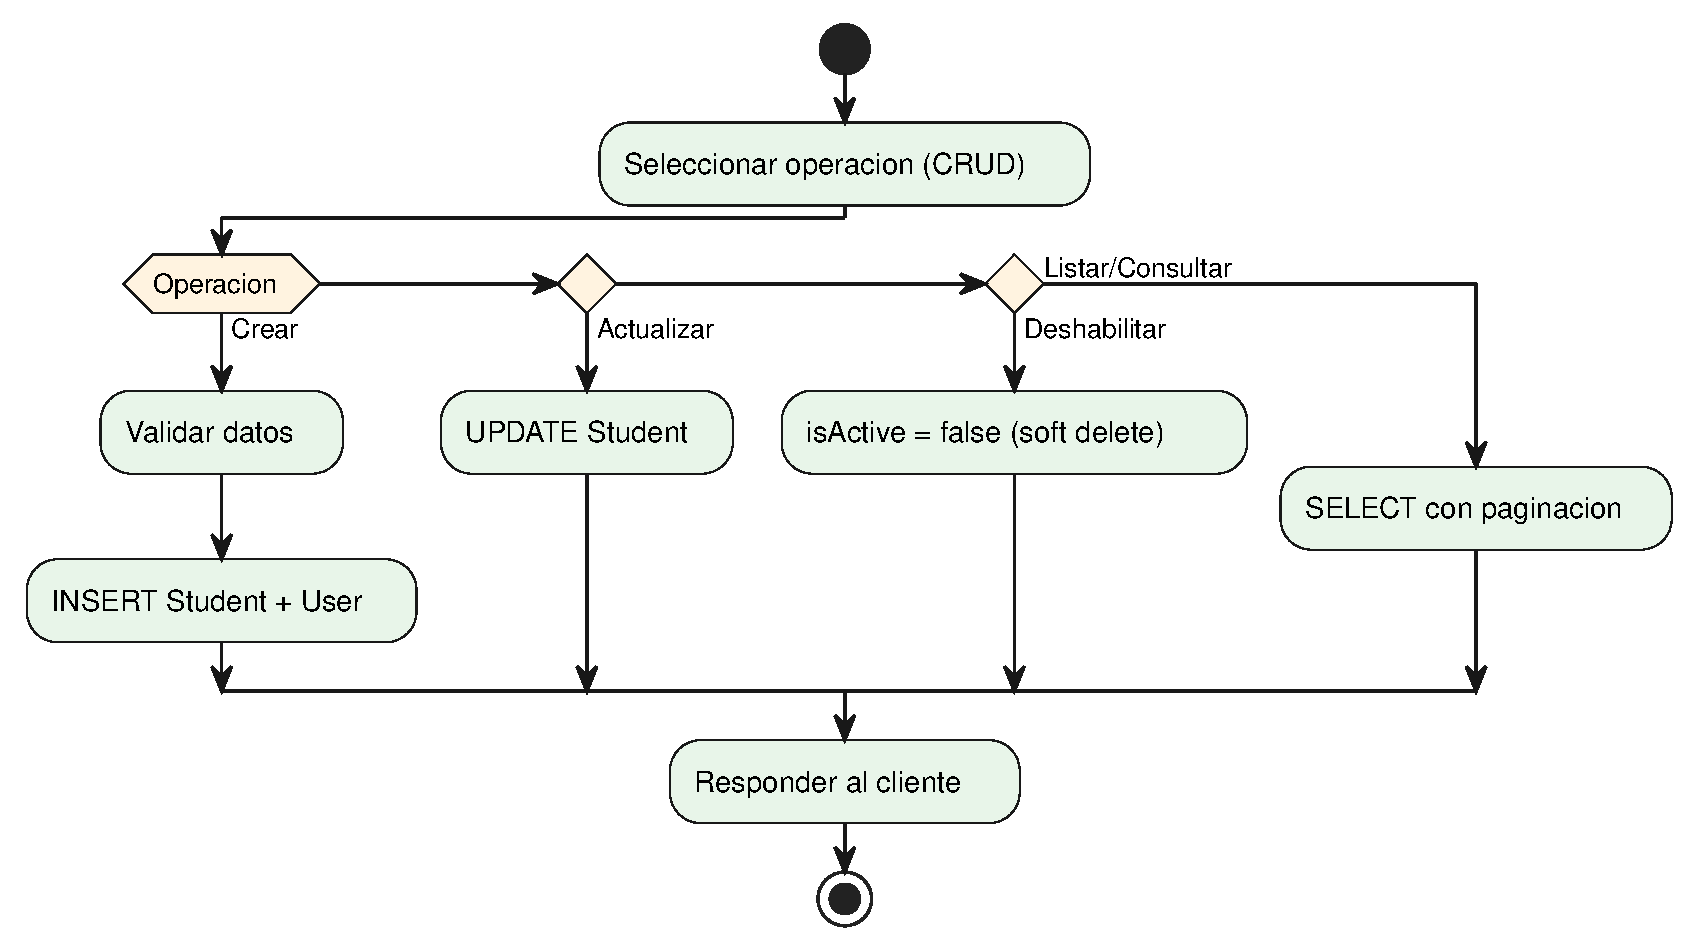
\includegraphics[width=\linewidth,height=0.46\textheight,keepaspectratio]{cu/cu05-act.pdf}\caption{Diagrama de actividades --- CU-05}\end{figure}

\subsection{CU-06 --- Importar estudiantes desde Excel}

\noindent\textbf{Endpoint(s):} \texttt{POST /api/students/import}\par\vspace{4pt}

\begin{table}[H]\centering\small
\caption{Ficha del caso de uso CU-06 --- Importar estudiantes desde Excel}
\begin{tabularx}{\textwidth}{L{0.26\textwidth} X}
\toprule
\textbf{Campo} & \textbf{Descripcion} \\ \midrule
Objetivo del contexto & Permitir al administrador cargar masivamente estudiantes a partir de un archivo Excel. \\ \midrule
Precondiciones & El administrador debe estar autenticado; el archivo debe tener el formato esperado. \\ \midrule
Condicion de exito & Se crean los estudiantes de las filas validas y se reporta el resultado. \\ \midrule
Condicion de fracaso & El archivo es invalido o no contiene filas procesables. \\ \midrule
Actores principales & Administrador \\ \midrule
Actores secundarios & Libreria de parseo xlsx \\
\bottomrule\end{tabularx}\end{table}
\begin{table}[H]\centering\small
\caption{Flujo principal de CU-06}
\begin{tabularx}{\textwidth}{C{0.10\textwidth} X}
\toprule \textbf{Paso} & \textbf{Accion} \\ \midrule
1 & El administrador sube un archivo .xlsx. \\
2 & El sistema parsea las filas del archivo. \\
3 & Por cada fila valida, el sistema crea el estudiante y su usuario. \\
4 & El sistema acumula errores de las filas invalidas. \\
5 & El sistema responde con un resumen (creados/errores). \\
\bottomrule\end{tabularx}\end{table}
\begin{table}[H]\centering\small
\caption{Extensiones (flujos alternativos) de CU-06}
\begin{tabularx}{\textwidth}{C{0.10\textwidth} X}
\toprule \textbf{Paso} & \textbf{Accion} \\ \midrule
2.1 & Archivo invalido o vacio $\rightarrow$ HTTP 400. \\
3.1 & Fila con datos invalidos $\rightarrow$ se registra el error y continua. \\
\bottomrule\end{tabularx}\end{table}
\begin{figure}[H]\centering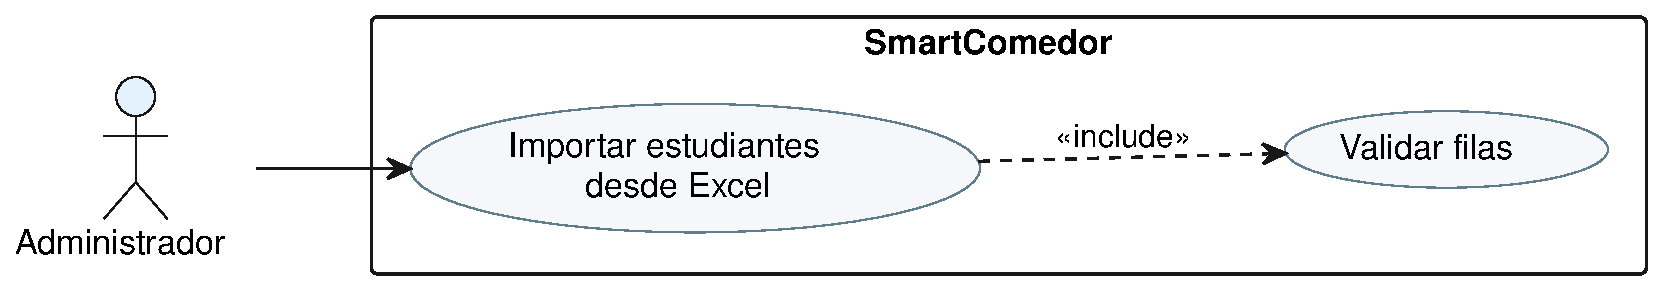
\includegraphics[width=\linewidth,height=0.30\textheight,keepaspectratio]{cu/cu06-uc.pdf}\caption{Diagrama de caso de uso --- CU-06}\end{figure}
\begin{figure}[H]\centering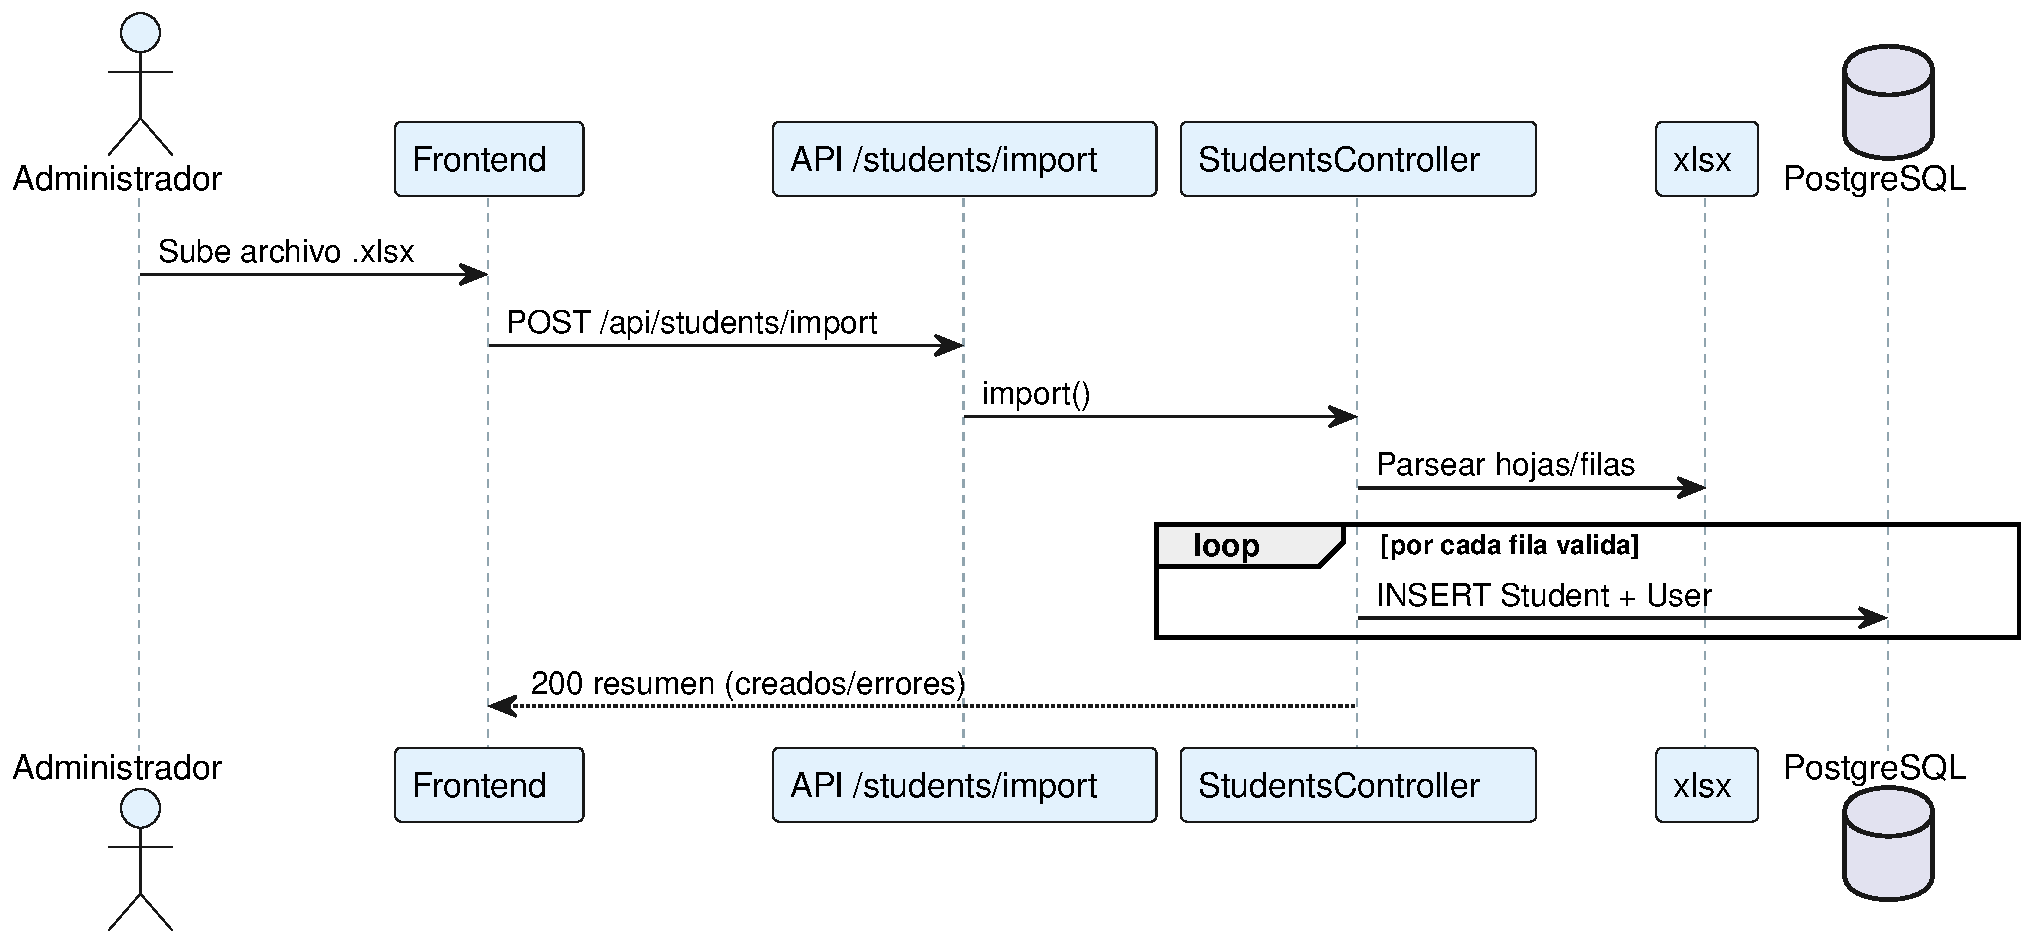
\includegraphics[width=\linewidth,height=0.42\textheight,keepaspectratio]{cu/cu06-seq.pdf}\caption{Diagrama de secuencia --- CU-06}\end{figure}
\begin{figure}[H]\centering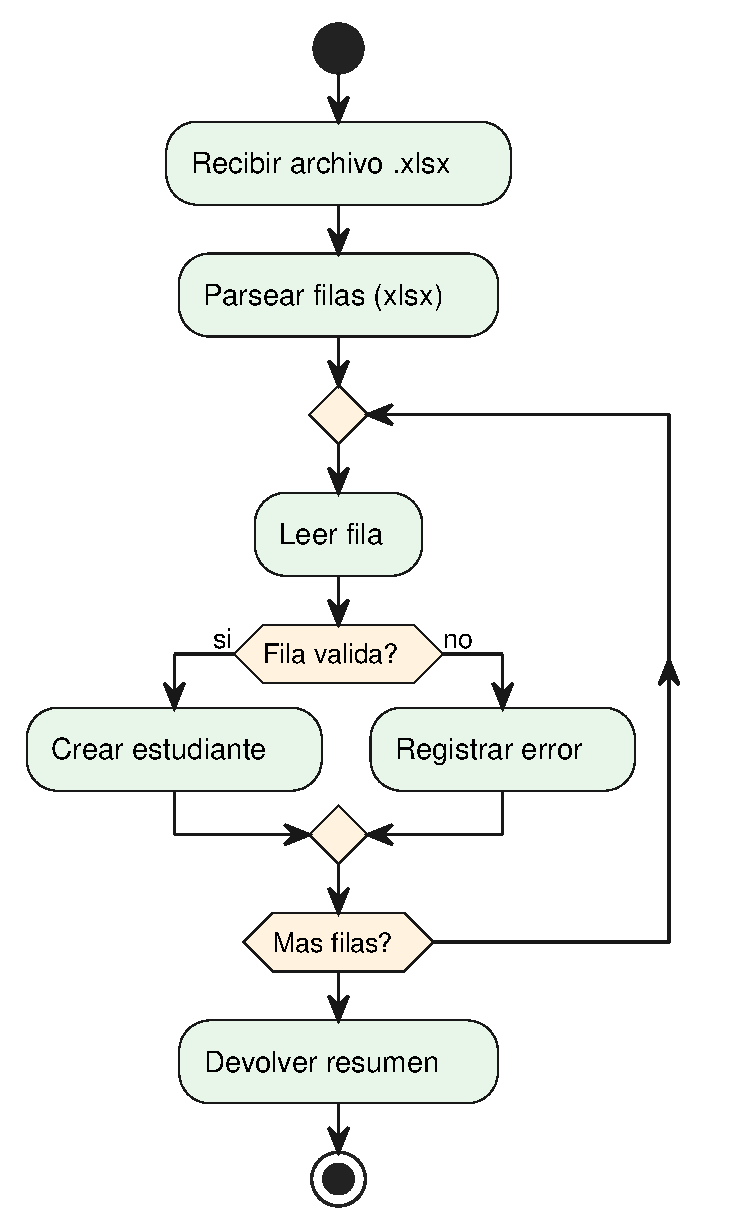
\includegraphics[width=\linewidth,height=0.46\textheight,keepaspectratio]{cu/cu06-act.pdf}\caption{Diagrama de actividades --- CU-06}\end{figure}

\subsection{CU-07 --- Validar SISBEN}

\noindent\textbf{Endpoint(s):} \texttt{POST /api/students/:id/validate-sisben}\par\vspace{4pt}

\begin{table}[H]\centering\small
\caption{Ficha del caso de uso CU-07 --- Validar SISBEN}
\begin{tabularx}{\textwidth}{L{0.26\textwidth} X}
\toprule
\textbf{Campo} & \textbf{Descripcion} \\ \midrule
Objetivo del contexto & Permitir al administrador validar la elegibilidad del estudiante cotejando el documento SISBEN con la cedula registrada. \\ \midrule
Precondiciones & El estudiante debe existir y tener documentos adjuntos. \\ \midrule
Condicion de exito & El estudiante queda con SISBEN validado. \\ \midrule
Condicion de fracaso & Existen discrepancias entre los documentos. \\ \midrule
Actores principales & Administrador \\ \midrule
Actores secundarios & Servicio de validacion SISBEN (PDF/OCR) \\
\bottomrule\end{tabularx}\end{table}
\begin{table}[H]\centering\small
\caption{Flujo principal de CU-07}
\begin{tabularx}{\textwidth}{C{0.10\textwidth} X}
\toprule \textbf{Paso} & \textbf{Accion} \\ \midrule
1 & El administrador solicita validar el SISBEN del estudiante. \\
2 & El sistema extrae el texto del documento (pdf-parse u OCR). \\
3 & El sistema normaliza y coteja cedula, nombre y apellido. \\
4 & Si todo coincide, marca isValidatedSisben = true y responde 200. \\
\bottomrule\end{tabularx}\end{table}
\begin{table}[H]\centering\small
\caption{Extensiones (flujos alternativos) de CU-07}
\begin{tabularx}{\textwidth}{C{0.10\textwidth} X}
\toprule \textbf{Paso} & \textbf{Accion} \\ \midrule
1.1 & Estudiante no encontrado $\rightarrow$ HTTP 404. \\
3.1 & Inconsistencia $\rightarrow$ validated=false con el detalle de cada discrepancia. \\
\bottomrule\end{tabularx}\end{table}
\begin{figure}[H]\centering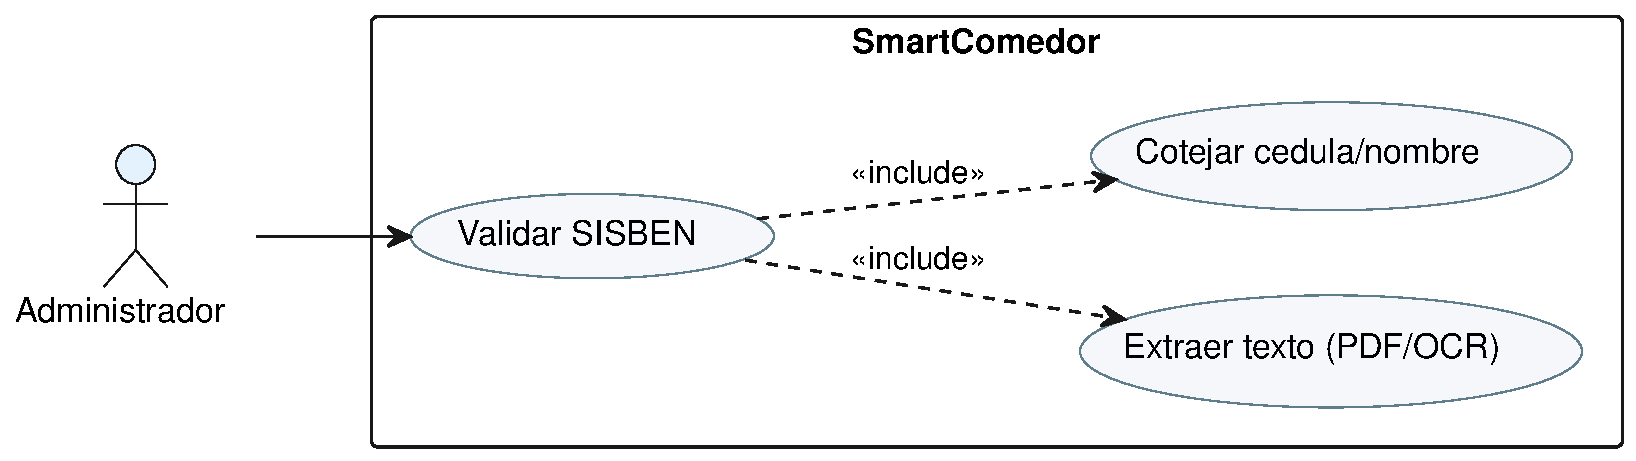
\includegraphics[width=\linewidth,height=0.30\textheight,keepaspectratio]{cu/cu07-uc.pdf}\caption{Diagrama de caso de uso --- CU-07}\end{figure}
\begin{figure}[H]\centering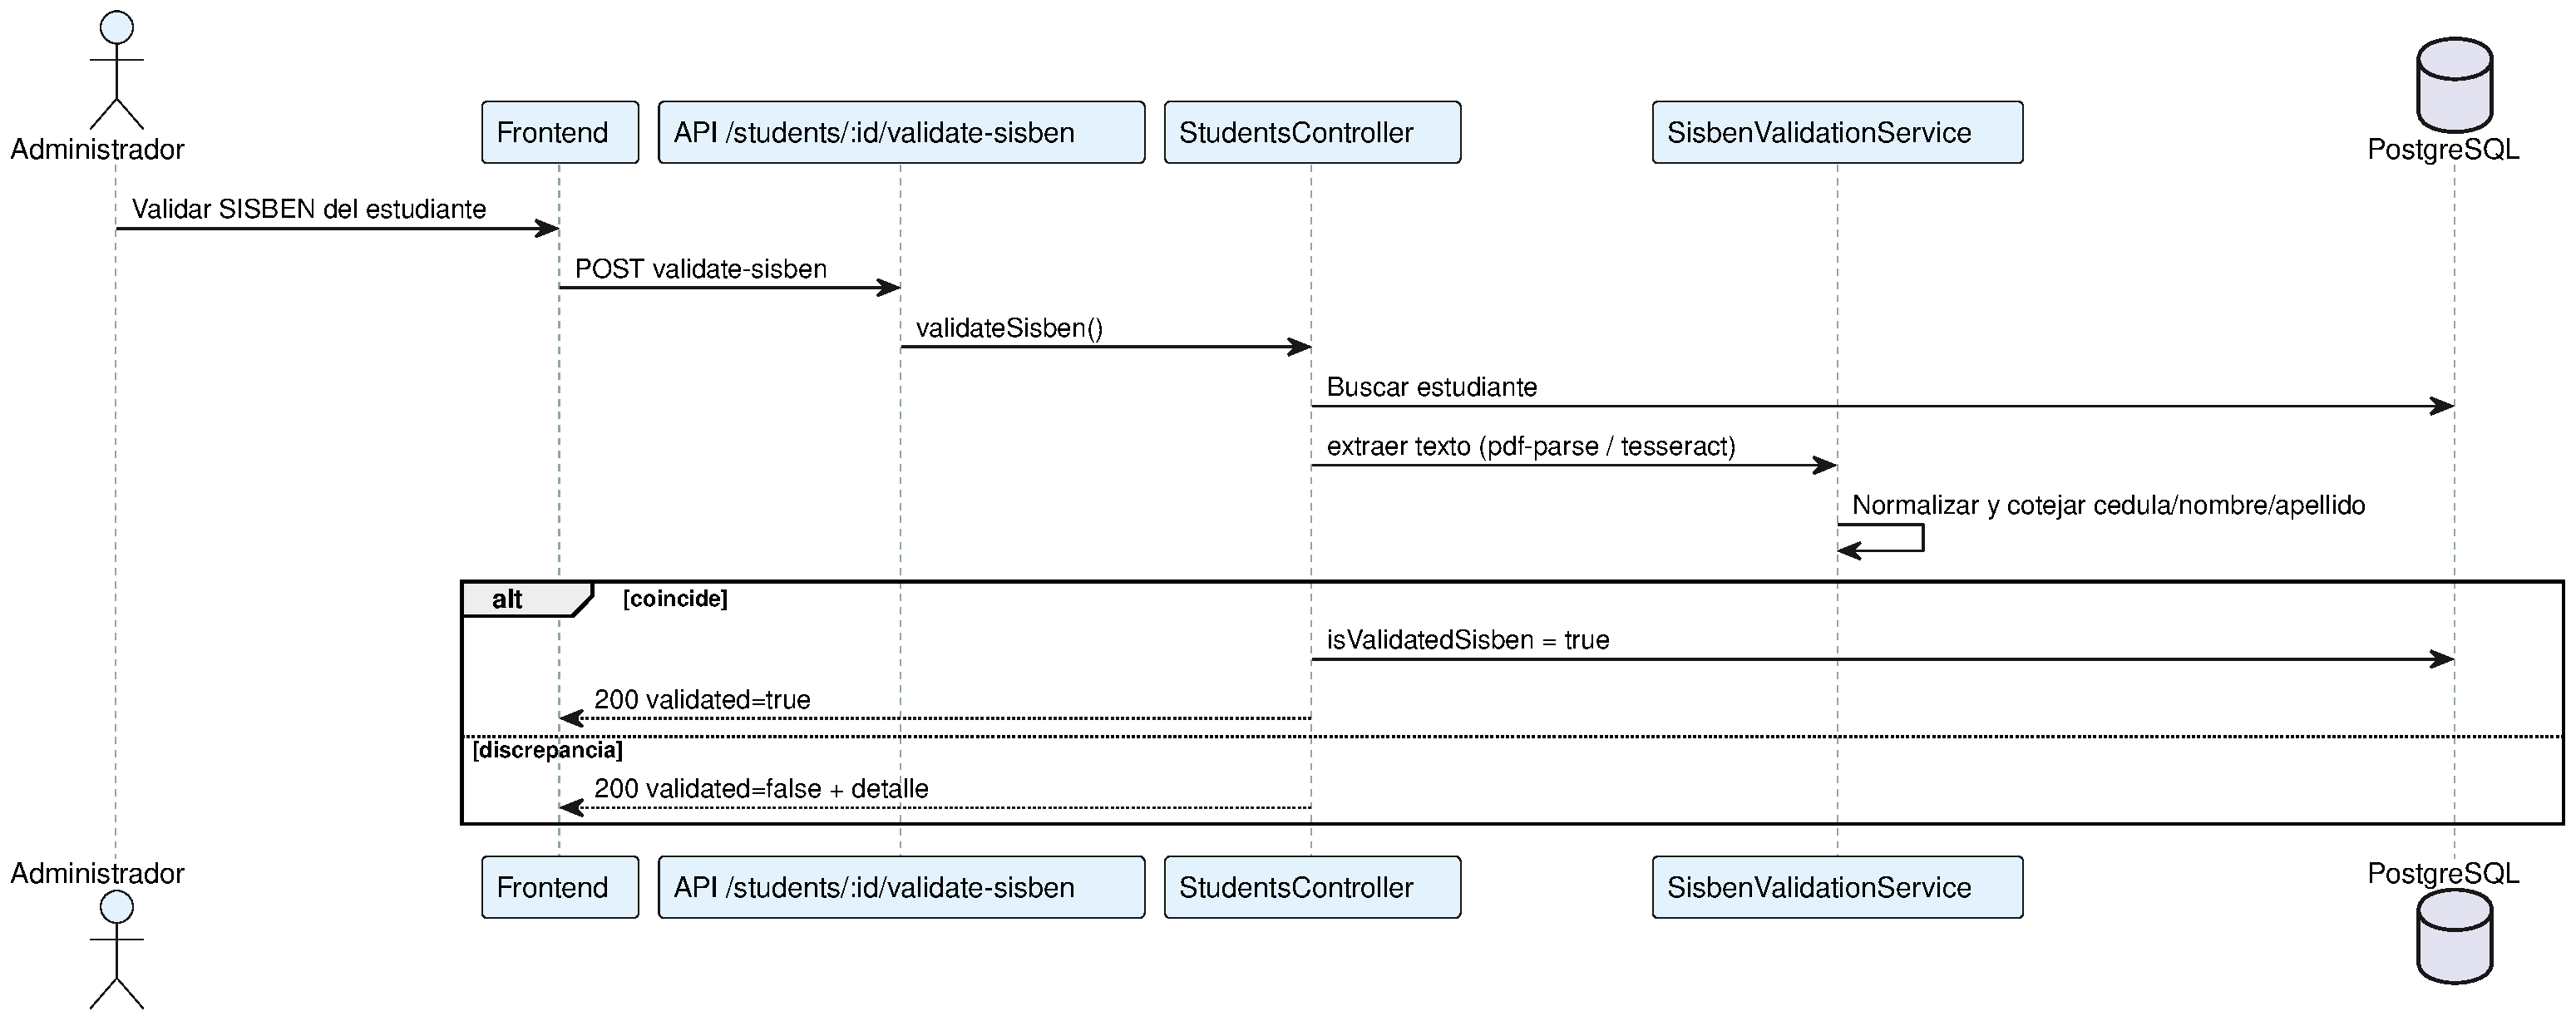
\includegraphics[width=\linewidth,height=0.42\textheight,keepaspectratio]{cu/cu07-seq.pdf}\caption{Diagrama de secuencia --- CU-07}\end{figure}
\begin{figure}[H]\centering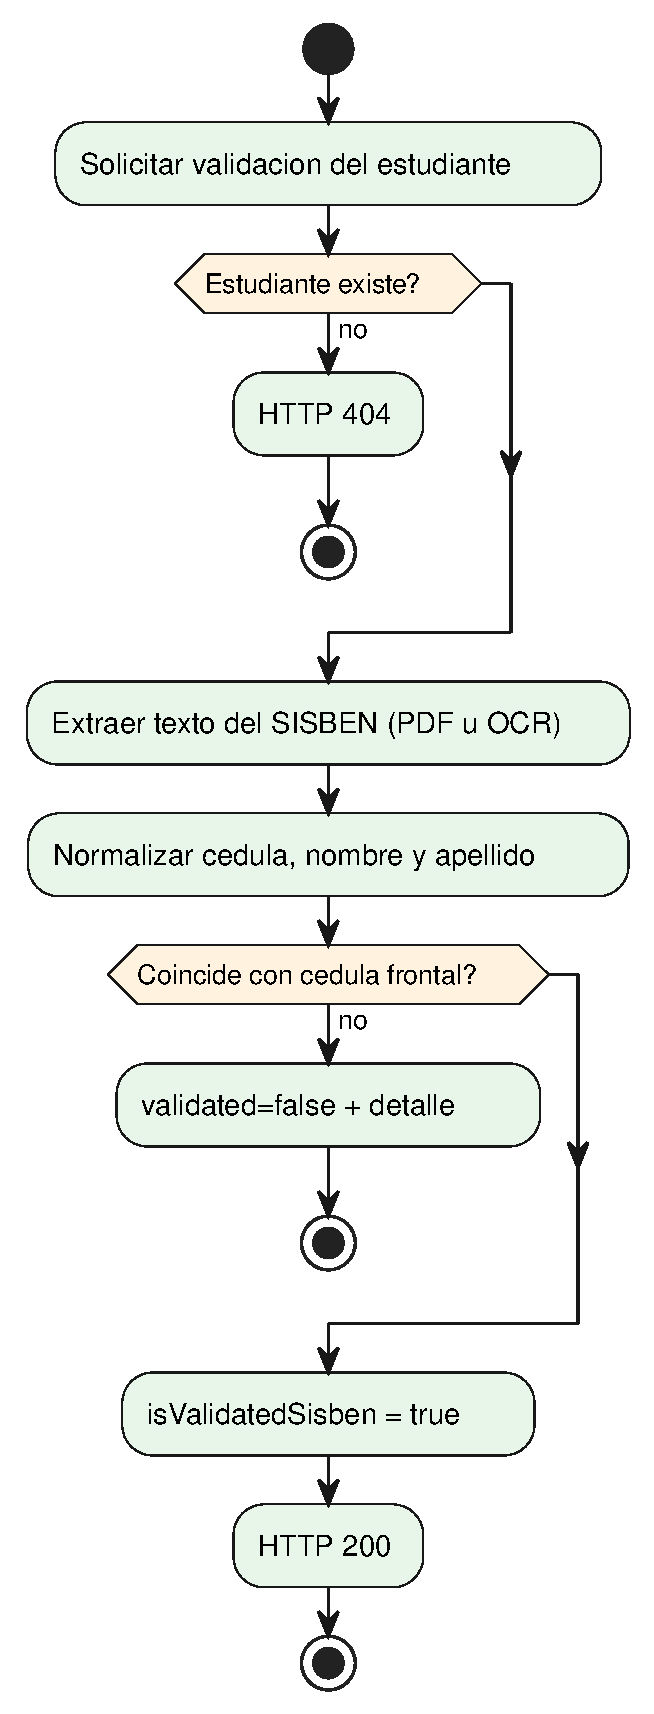
\includegraphics[width=\linewidth,height=0.46\textheight,keepaspectratio]{cu/cu07-act.pdf}\caption{Diagrama de actividades --- CU-07}\end{figure}

\subsection{CU-08 --- Gestionar supervisores}

\noindent\textbf{Endpoint(s):} \texttt{GET/POST/PUT/PATCH/DELETE /api/supervisors}\par\vspace{4pt}

\begin{table}[H]\centering\small
\caption{Ficha del caso de uso CU-08 --- Gestionar supervisores}
\begin{tabularx}{\textwidth}{L{0.26\textwidth} X}
\toprule
\textbf{Campo} & \textbf{Descripcion} \\ \midrule
Objetivo del contexto & Permitir al administrador crear, actualizar, cambiar de estado y deshabilitar supervisores, y consultar sus bitacoras. \\ \midrule
Precondiciones & El administrador debe estar autenticado con rol admin. \\ \midrule
Condicion de exito & El supervisor se crea o actualiza segun la operacion. \\ \midrule
Condicion de fracaso & Datos invalidos o supervisor inexistente. \\ \midrule
Actores principales & Administrador \\ \midrule
Actores secundarios & Base de datos \\
\bottomrule\end{tabularx}\end{table}
\begin{table}[H]\centering\small
\caption{Flujo principal de CU-08}
\begin{tabularx}{\textwidth}{C{0.10\textwidth} X}
\toprule \textbf{Paso} & \textbf{Accion} \\ \midrule
1 & El administrador selecciona la operacion sobre el supervisor. \\
2 & Para crear, el sistema genera una contrasena temporal cifrada. \\
3 & El sistema persiste el usuario con rol supervisor. \\
4 & Para cambiar estado, actualiza isActive/isAuthorized. \\
5 & El sistema responde con el resultado. \\
\bottomrule\end{tabularx}\end{table}
\begin{table}[H]\centering\small
\caption{Extensiones (flujos alternativos) de CU-08}
\begin{tabularx}{\textwidth}{C{0.10\textwidth} X}
\toprule \textbf{Paso} & \textbf{Accion} \\ \midrule
3.1 & Correo duplicado $\rightarrow$ HTTP 400. \\
4.1 & Supervisor inexistente $\rightarrow$ HTTP 404. \\
\bottomrule\end{tabularx}\end{table}
\begin{figure}[H]\centering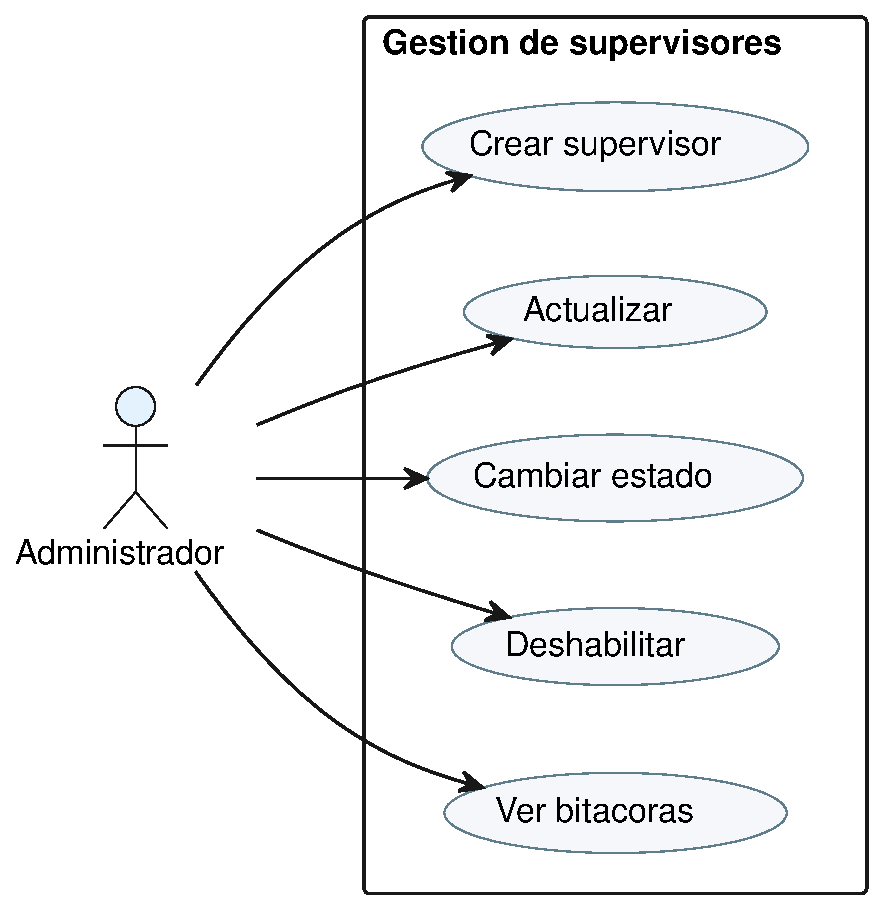
\includegraphics[width=\linewidth,height=0.30\textheight,keepaspectratio]{cu/cu08-uc.pdf}\caption{Diagrama de caso de uso --- CU-08}\end{figure}
\begin{figure}[H]\centering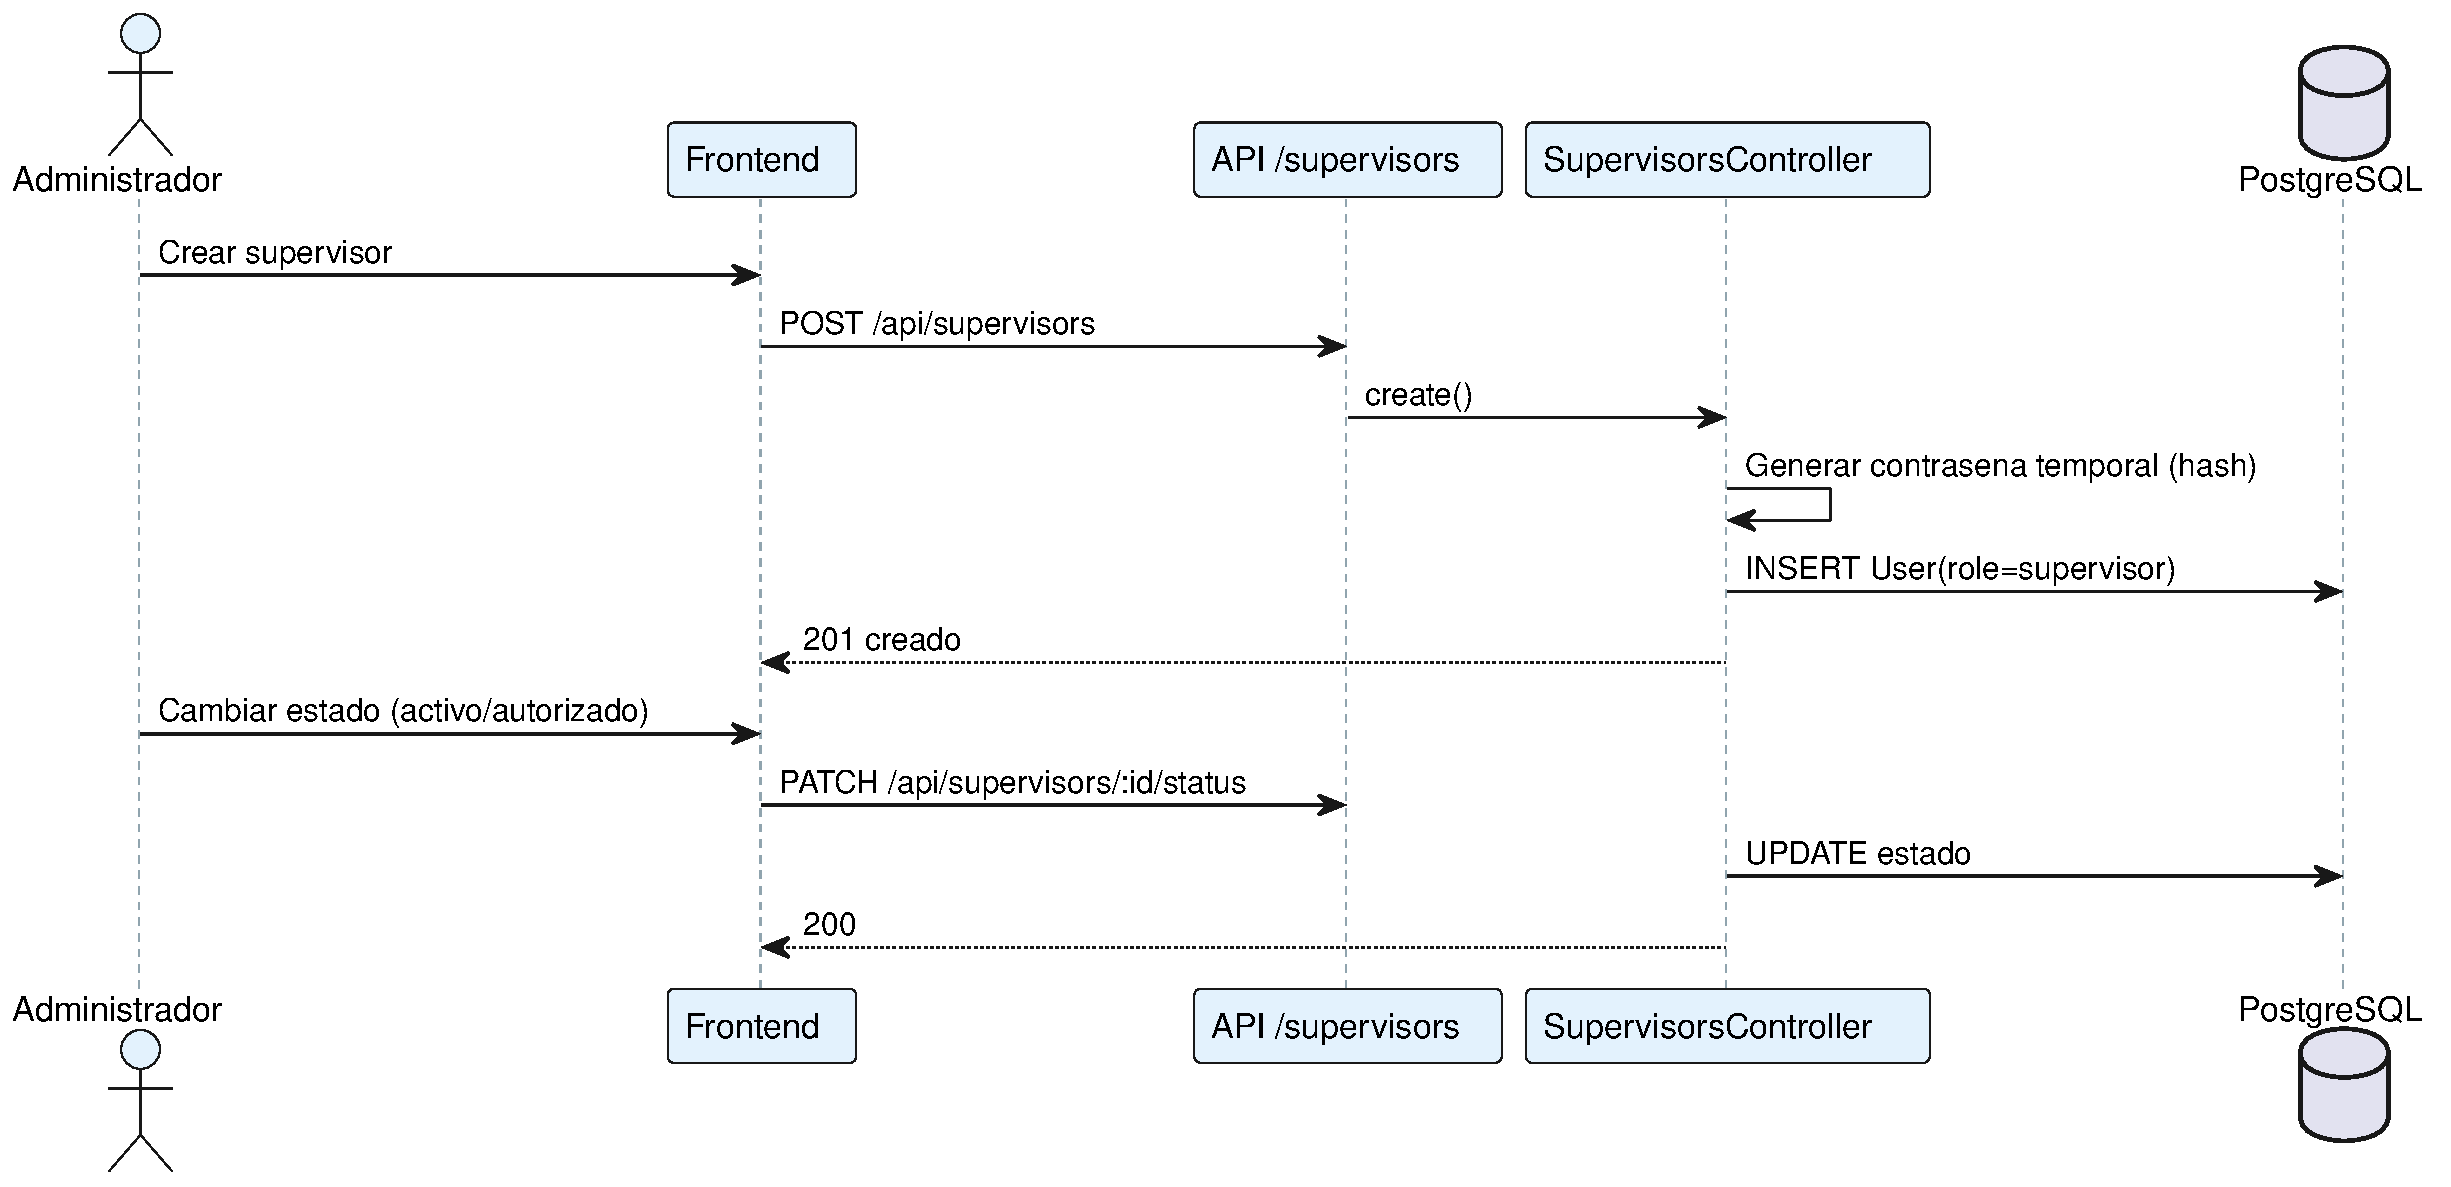
\includegraphics[width=\linewidth,height=0.42\textheight,keepaspectratio]{cu/cu08-seq.pdf}\caption{Diagrama de secuencia --- CU-08}\end{figure}
\begin{figure}[H]\centering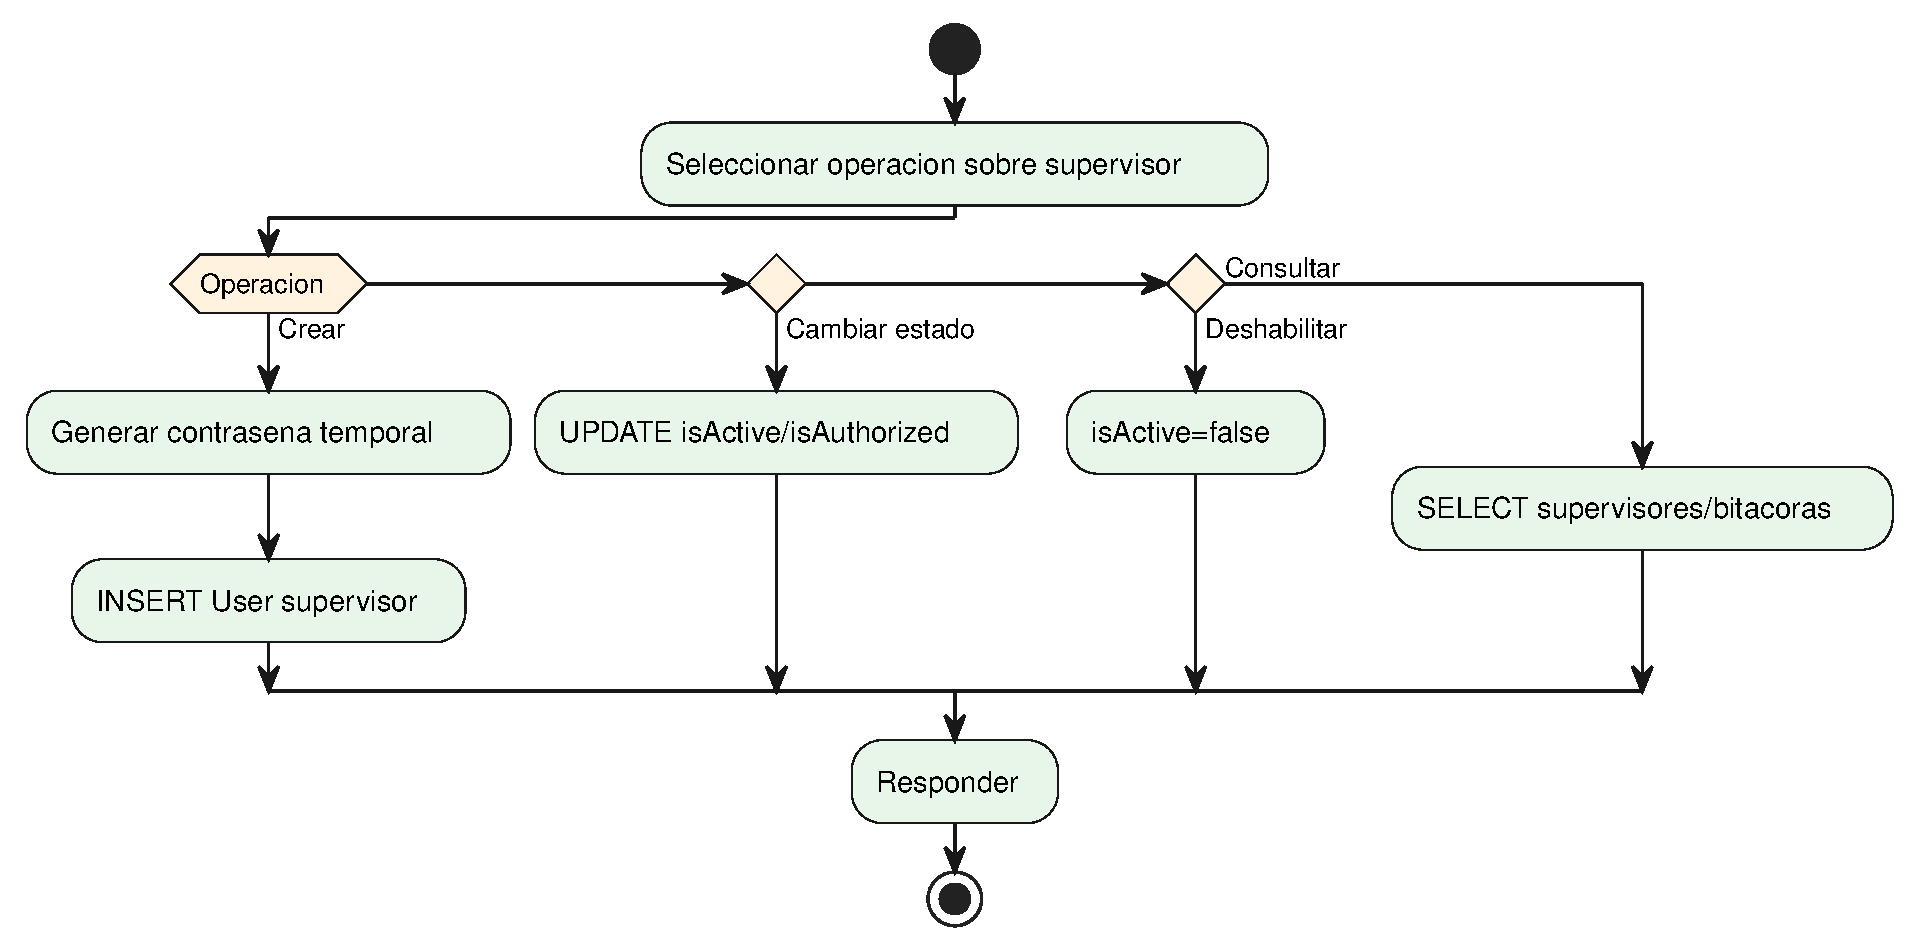
\includegraphics[width=\linewidth,height=0.46\textheight,keepaspectratio]{cu/cu08-act.pdf}\caption{Diagrama de actividades --- CU-08}\end{figure}

\subsection{CU-09 --- Invitar supervisor / unirse por invitacion}

\noindent\textbf{Endpoint(s):} \texttt{POST /api/supervisors/invite, POST /api/supervisors/join}\par\vspace{4pt}

\begin{table}[H]\centering\small
\caption{Ficha del caso de uso CU-09 --- Invitar supervisor / unirse por invitacion}
\begin{tabularx}{\textwidth}{L{0.26\textwidth} X}
\toprule
\textbf{Campo} & \textbf{Descripcion} \\ \midrule
Objetivo del contexto & Permitir al administrador invitar supervisores por correo y a estos crear su cuenta mediante un enlace temporal. \\ \midrule
Precondiciones & El administrador debe estar autenticado; la invitacion debe estar vigente. \\ \midrule
Condicion de exito & El supervisor crea su cuenta a partir de la invitacion. \\ \midrule
Condicion de fracaso & El token de invitacion es invalido o expirado. \\ \midrule
Actores principales & Administrador, Supervisor \\ \midrule
Actores secundarios & Servicio de correo \\
\bottomrule\end{tabularx}\end{table}
\begin{table}[H]\centering\small
\caption{Flujo principal de CU-09}
\begin{tabularx}{\textwidth}{C{0.10\textwidth} X}
\toprule \textbf{Paso} & \textbf{Accion} \\ \midrule
1 & El administrador genera una invitacion indicando el correo. \\
2 & El sistema crea un token con vigencia de 48 horas. \\
3 & El sistema envia el enlace de invitacion por correo. \\
4 & El supervisor abre el enlace y completa sus datos. \\
5 & El sistema valida el token y crea la cuenta de supervisor. \\
\bottomrule\end{tabularx}\end{table}
\begin{table}[H]\centering\small
\caption{Extensiones (flujos alternativos) de CU-09}
\begin{tabularx}{\textwidth}{C{0.10\textwidth} X}
\toprule \textbf{Paso} & \textbf{Accion} \\ \midrule
5.1 & Token vencido $\rightarrow$ HTTP 400. \\
5.2 & Correo duplicado $\rightarrow$ HTTP 400. \\
\bottomrule\end{tabularx}\end{table}
\begin{figure}[H]\centering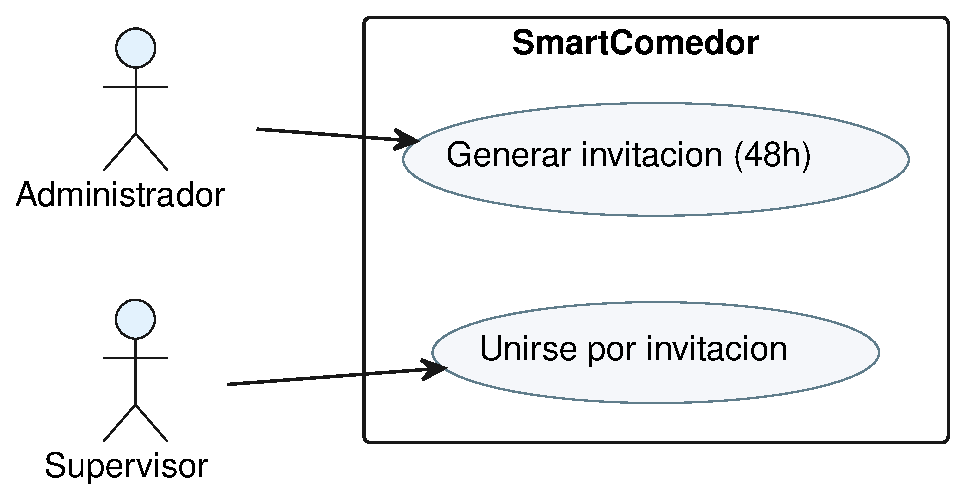
\includegraphics[width=\linewidth,height=0.30\textheight,keepaspectratio]{cu/cu09-uc.pdf}\caption{Diagrama de caso de uso --- CU-09}\end{figure}
\begin{figure}[H]\centering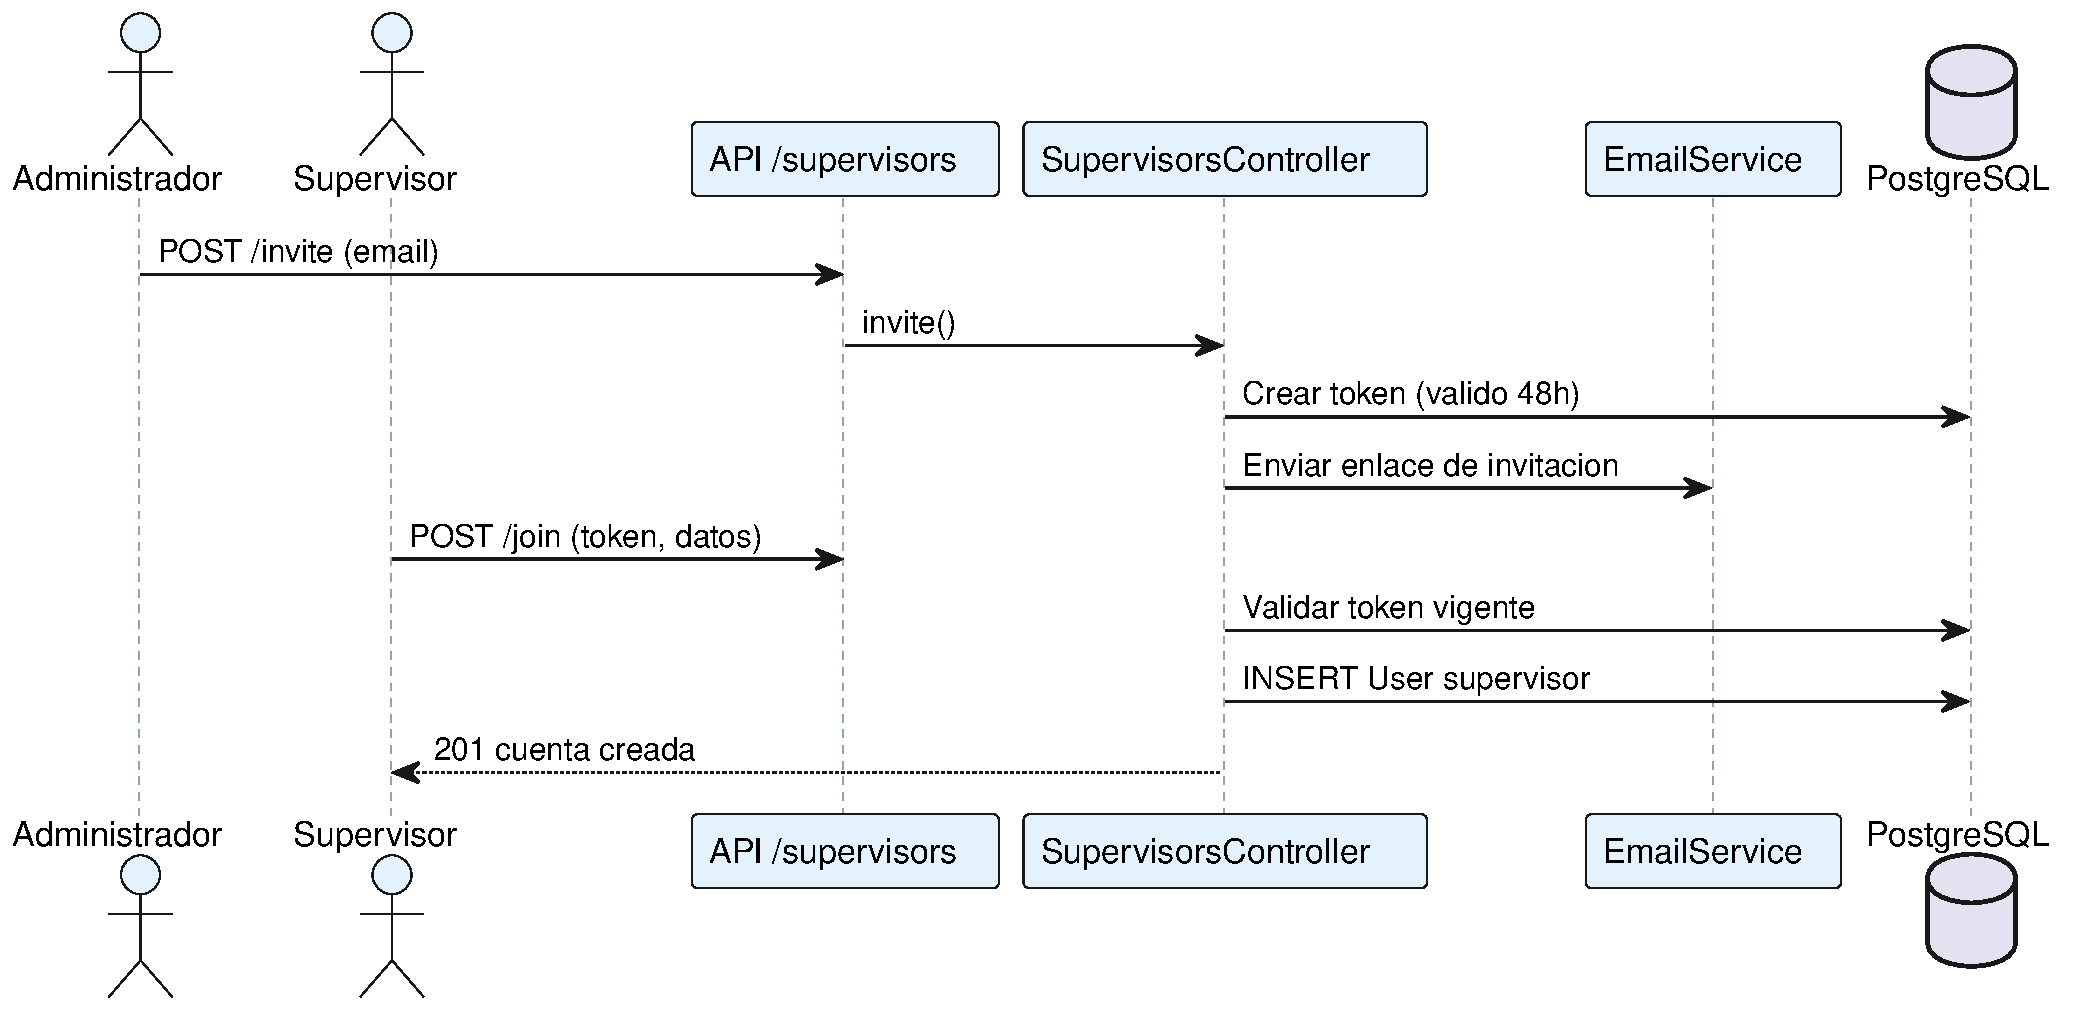
\includegraphics[width=\linewidth,height=0.42\textheight,keepaspectratio]{cu/cu09-seq.pdf}\caption{Diagrama de secuencia --- CU-09}\end{figure}
\begin{figure}[H]\centering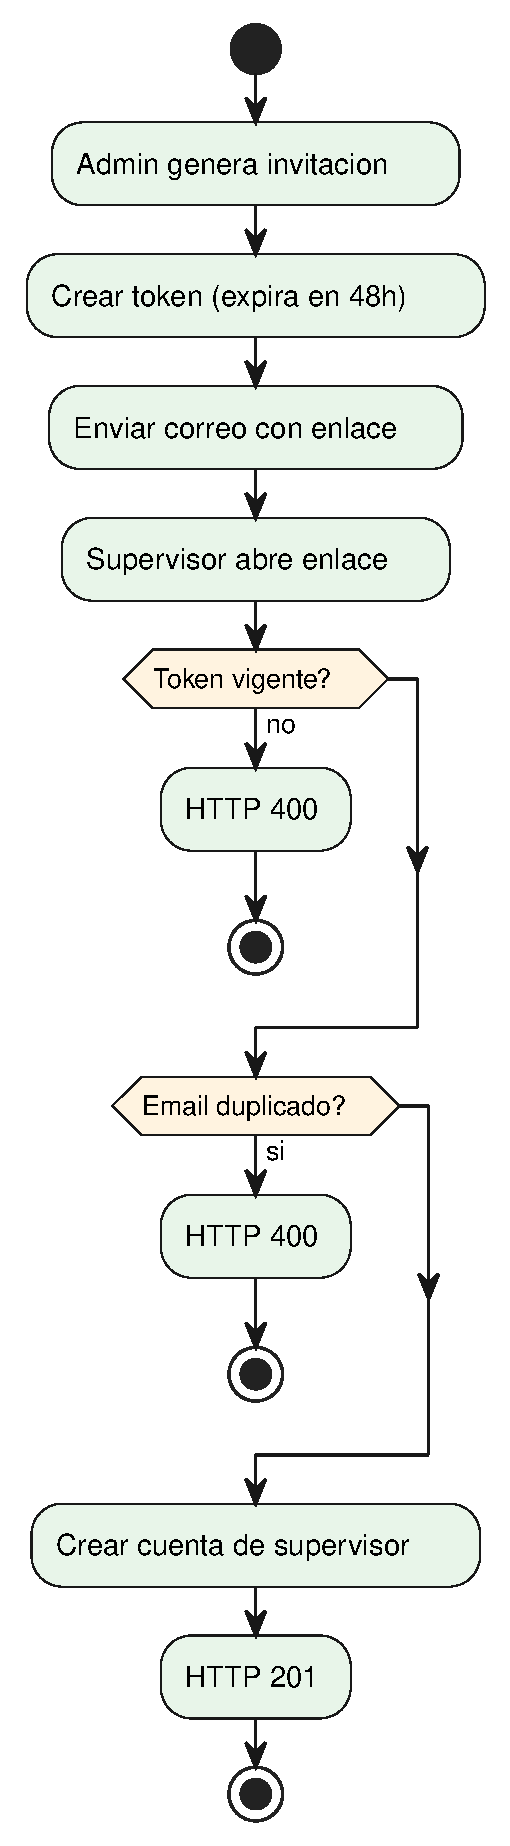
\includegraphics[width=\linewidth,height=0.46\textheight,keepaspectratio]{cu/cu09-act.pdf}\caption{Diagrama de actividades --- CU-09}\end{figure}

\subsection{CU-10 --- Asignar estudiantes a supervisor}

\noindent\textbf{Endpoint(s):} \texttt{POST/DELETE /api/supervisors/:id/assignments}\par\vspace{4pt}

\begin{table}[H]\centering\small
\caption{Ficha del caso de uso CU-10 --- Asignar estudiantes a supervisor}
\begin{tabularx}{\textwidth}{L{0.26\textwidth} X}
\toprule
\textbf{Campo} & \textbf{Descripcion} \\ \midrule
Objetivo del contexto & Permitir al administrador asociar estudiantes a un supervisor para delimitar su ambito de supervision. \\ \midrule
Precondiciones & El supervisor y el estudiante deben existir. \\ \midrule
Condicion de exito & Se crea la relacion supervisor-estudiante. \\ \midrule
Condicion de fracaso & La asignacion ya existe. \\ \midrule
Actores principales & Administrador \\ \midrule
Actores secundarios & Base de datos \\
\bottomrule\end{tabularx}\end{table}
\begin{table}[H]\centering\small
\caption{Flujo principal de CU-10}
\begin{tabularx}{\textwidth}{C{0.10\textwidth} X}
\toprule \textbf{Paso} & \textbf{Accion} \\ \midrule
1 & El administrador selecciona un supervisor y un estudiante. \\
2 & El sistema verifica que la asignacion no exista. \\
3 & El sistema crea el registro de asignacion (N:M). \\
4 & El sistema responde 201. \\
\bottomrule\end{tabularx}\end{table}
\begin{table}[H]\centering\small
\caption{Extensiones (flujos alternativos) de CU-10}
\begin{tabularx}{\textwidth}{C{0.10\textwidth} X}
\toprule \textbf{Paso} & \textbf{Accion} \\ \midrule
2.1 & Asignacion duplicada $\rightarrow$ HTTP 400. \\
\bottomrule\end{tabularx}\end{table}
\begin{figure}[H]\centering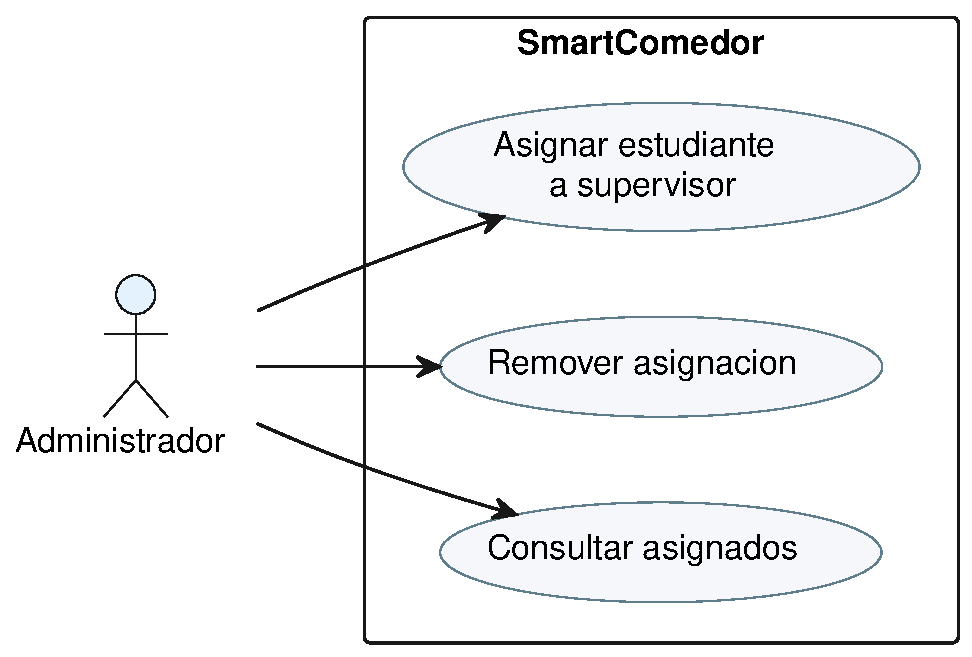
\includegraphics[width=\linewidth,height=0.30\textheight,keepaspectratio]{cu/cu10-uc.pdf}\caption{Diagrama de caso de uso --- CU-10}\end{figure}
\begin{figure}[H]\centering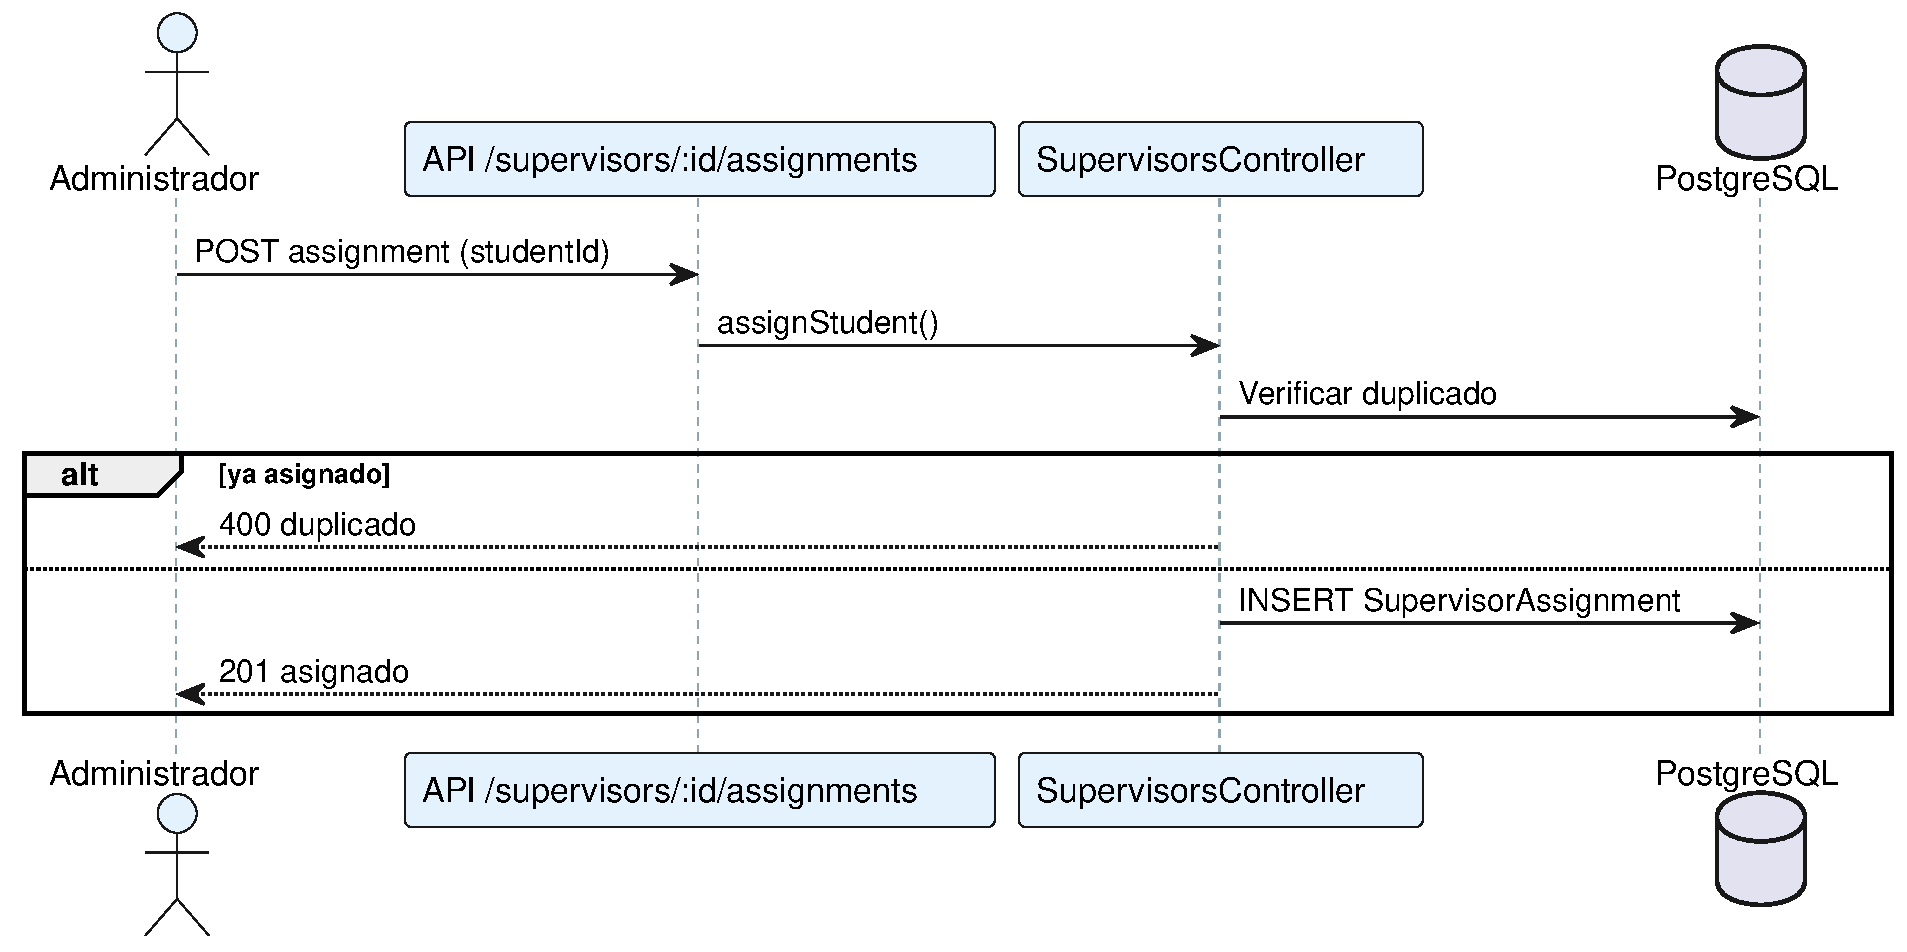
\includegraphics[width=\linewidth,height=0.42\textheight,keepaspectratio]{cu/cu10-seq.pdf}\caption{Diagrama de secuencia --- CU-10}\end{figure}
\begin{figure}[H]\centering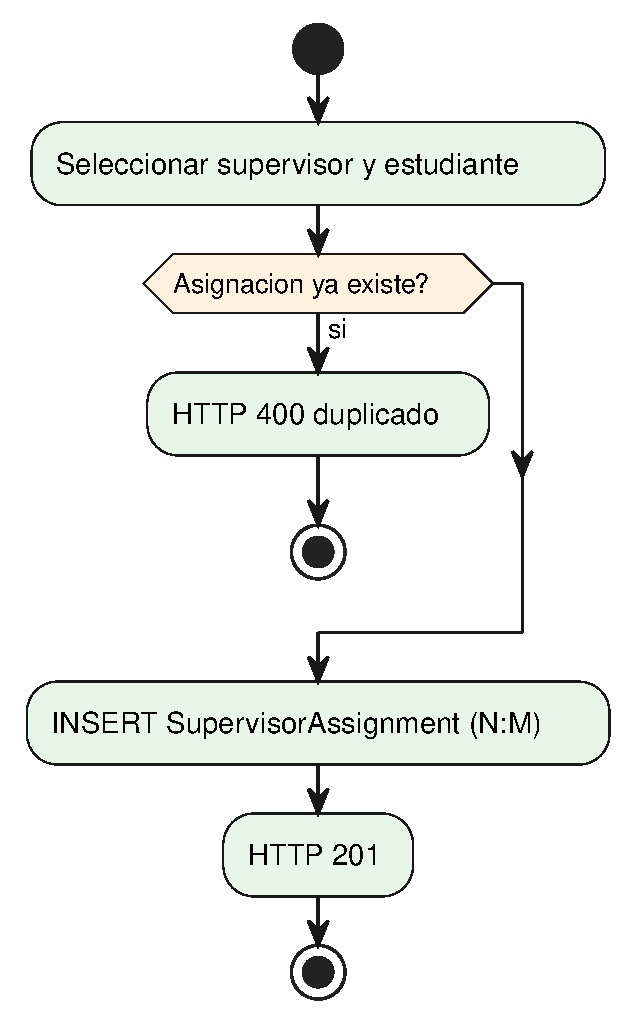
\includegraphics[width=\linewidth,height=0.46\textheight,keepaspectratio]{cu/cu10-act.pdf}\caption{Diagrama de actividades --- CU-10}\end{figure}

\subsection{CU-11 --- Subir pago y comprobantes}

\noindent\textbf{Endpoint(s):} \texttt{POST /api/payments, POST /api/payments/upload, POST /api/payments/calculate}\par\vspace{4pt}

\begin{table}[H]\centering\small
\caption{Ficha del caso de uso CU-11 --- Subir pago y comprobantes}
\begin{tabularx}{\textwidth}{L{0.26\textwidth} X}
\toprule
\textbf{Campo} & \textbf{Descripcion} \\ \midrule
Objetivo del contexto & Permitir al estudiante registrar un pago/recarga indicando el monto y adjuntando el comprobante, calculando los almuerzos incluidos. \\ \midrule
Precondiciones & El estudiante debe estar autenticado. \\ \midrule
Condicion de exito & Se crea un pago pendiente de verificacion con los almuerzos calculados. \\ \midrule
Condicion de fracaso & El monto es invalido (menor al precio de un almuerzo). \\ \midrule
Actores principales & Estudiante \\ \midrule
Actores secundarios & Almacenamiento de archivos \\
\bottomrule\end{tabularx}\end{table}
\begin{table}[H]\centering\small
\caption{Flujo principal de CU-11}
\begin{tabularx}{\textwidth}{C{0.10\textwidth} X}
\toprule \textbf{Paso} & \textbf{Accion} \\ \midrule
1 & El estudiante ingresa el monto y adjunta el comprobante. \\
2 & El sistema calcula almuerzos = piso(monto/2000). \\
3 & El sistema crea el pago con isVerified=false. \\
4 & El sistema responde 201. \\
\bottomrule\end{tabularx}\end{table}
\begin{table}[H]\centering\small
\caption{Extensiones (flujos alternativos) de CU-11}
\begin{tabularx}{\textwidth}{C{0.10\textwidth} X}
\toprule \textbf{Paso} & \textbf{Accion} \\ \midrule
2.1 & Monto menor a 2000 $\rightarrow$ HTTP 400. \\
\bottomrule\end{tabularx}\end{table}
\begin{figure}[H]\centering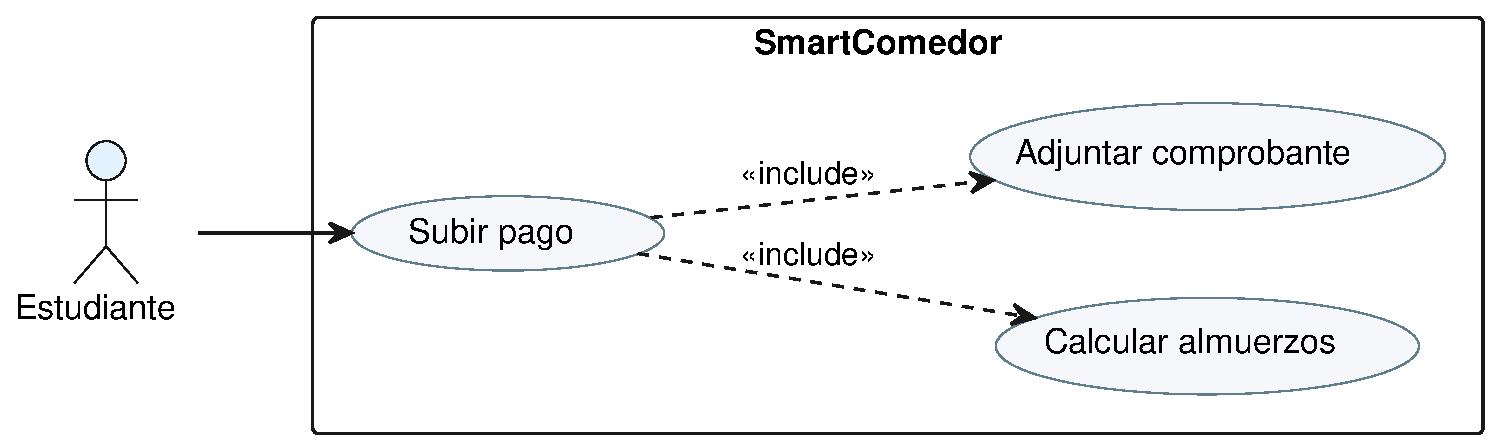
\includegraphics[width=\linewidth,height=0.30\textheight,keepaspectratio]{cu/cu11-uc.pdf}\caption{Diagrama de caso de uso --- CU-11}\end{figure}
\begin{figure}[H]\centering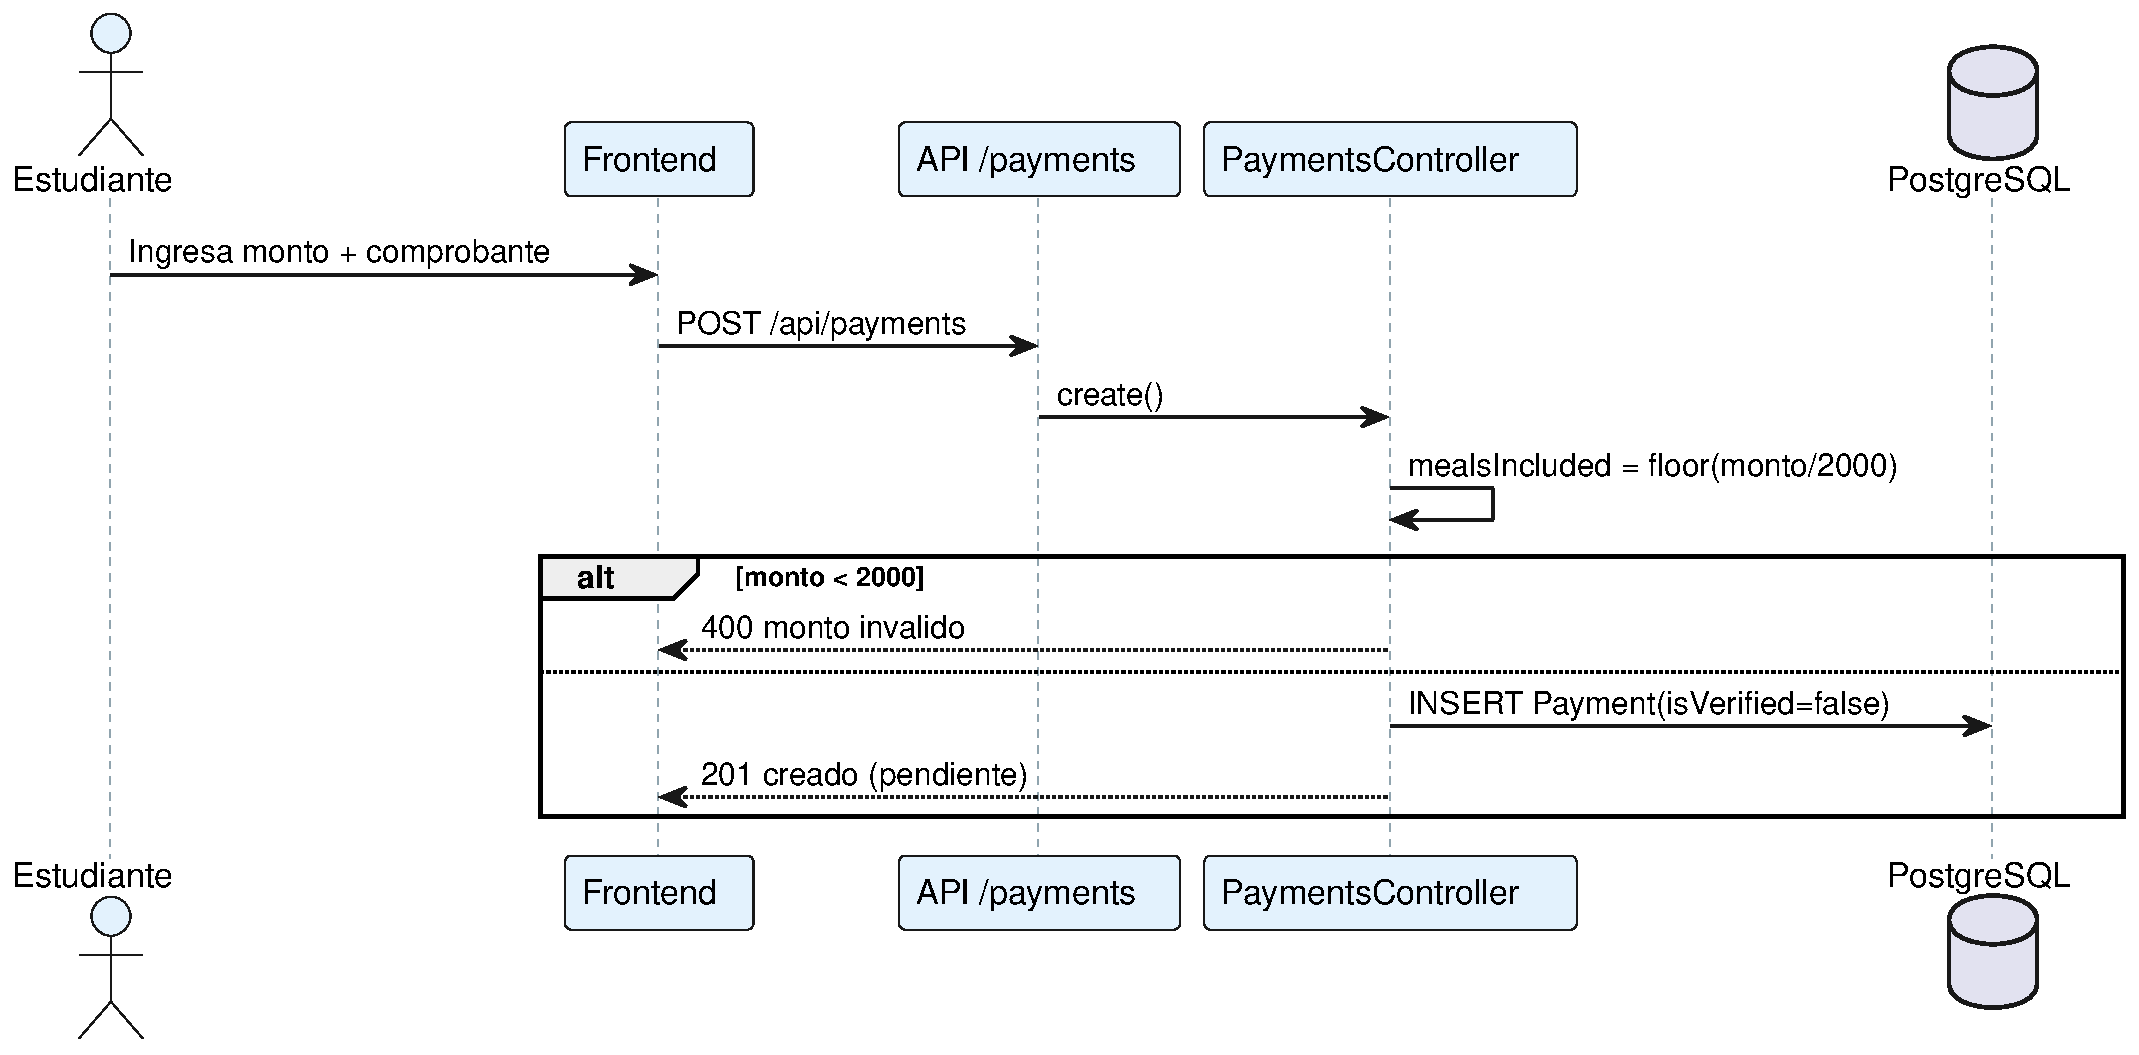
\includegraphics[width=\linewidth,height=0.42\textheight,keepaspectratio]{cu/cu11-seq.pdf}\caption{Diagrama de secuencia --- CU-11}\end{figure}
\begin{figure}[H]\centering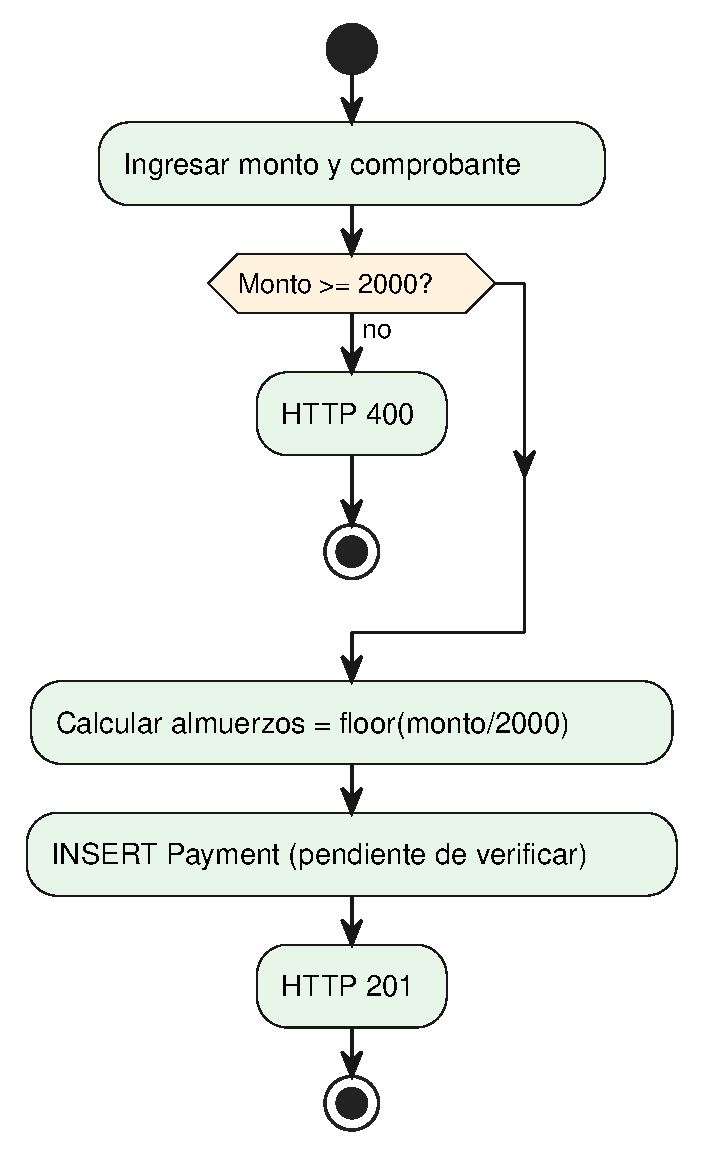
\includegraphics[width=\linewidth,height=0.46\textheight,keepaspectratio]{cu/cu11-act.pdf}\caption{Diagrama de actividades --- CU-11}\end{figure}

\subsection{CU-12 --- Verificar pago}

\noindent\textbf{Endpoint(s):} \texttt{PATCH /api/payments/:id/verify}\par\vspace{4pt}

\begin{table}[H]\centering\small
\caption{Ficha del caso de uso CU-12 --- Verificar pago}
\begin{tabularx}{\textwidth}{L{0.26\textwidth} X}
\toprule
\textbf{Campo} & \textbf{Descripcion} \\ \midrule
Objetivo del contexto & Permitir al administrador verificar un pago para habilitar los almuerzos del estudiante, dejando trazabilidad. \\ \midrule
Precondiciones & El pago debe existir y estar pendiente. \\ \midrule
Condicion de exito & El pago queda verificado y se registra en auditoria. \\ \midrule
Condicion de fracaso & El pago no existe. \\ \midrule
Actores principales & Administrador \\ \midrule
Actores secundarios & Servicio de auditoria \\
\bottomrule\end{tabularx}\end{table}
\begin{table}[H]\centering\small
\caption{Flujo principal de CU-12}
\begin{tabularx}{\textwidth}{C{0.10\textwidth} X}
\toprule \textbf{Paso} & \textbf{Accion} \\ \midrule
1 & El administrador selecciona el pago a verificar. \\
2 & El sistema verifica que el pago exista. \\
3 & El sistema marca isVerified=true (verifiedBy, verifiedAt). \\
4 & El sistema registra el evento en auditoria. \\
5 & El sistema responde 200. \\
\bottomrule\end{tabularx}\end{table}
\begin{table}[H]\centering\small
\caption{Extensiones (flujos alternativos) de CU-12}
\begin{tabularx}{\textwidth}{C{0.10\textwidth} X}
\toprule \textbf{Paso} & \textbf{Accion} \\ \midrule
2.1 & Pago inexistente $\rightarrow$ HTTP 404. \\
\bottomrule\end{tabularx}\end{table}
\begin{figure}[H]\centering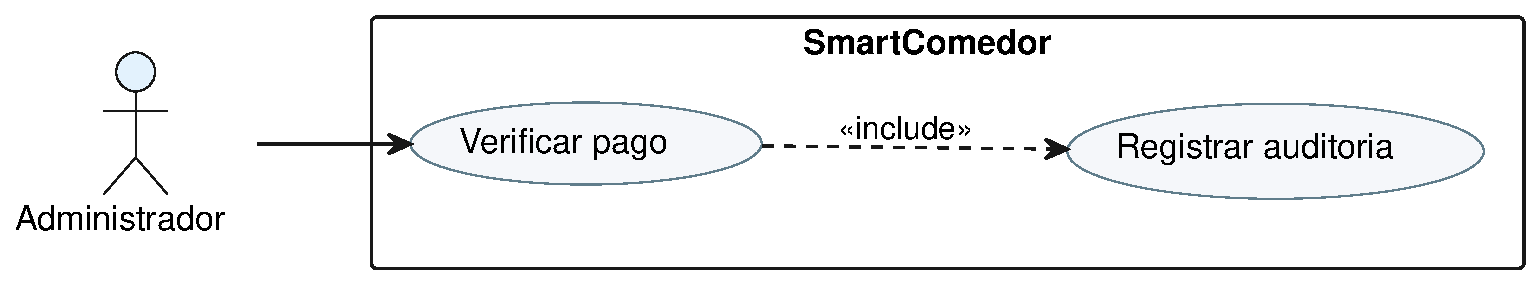
\includegraphics[width=\linewidth,height=0.30\textheight,keepaspectratio]{cu/cu12-uc.pdf}\caption{Diagrama de caso de uso --- CU-12}\end{figure}
\begin{figure}[H]\centering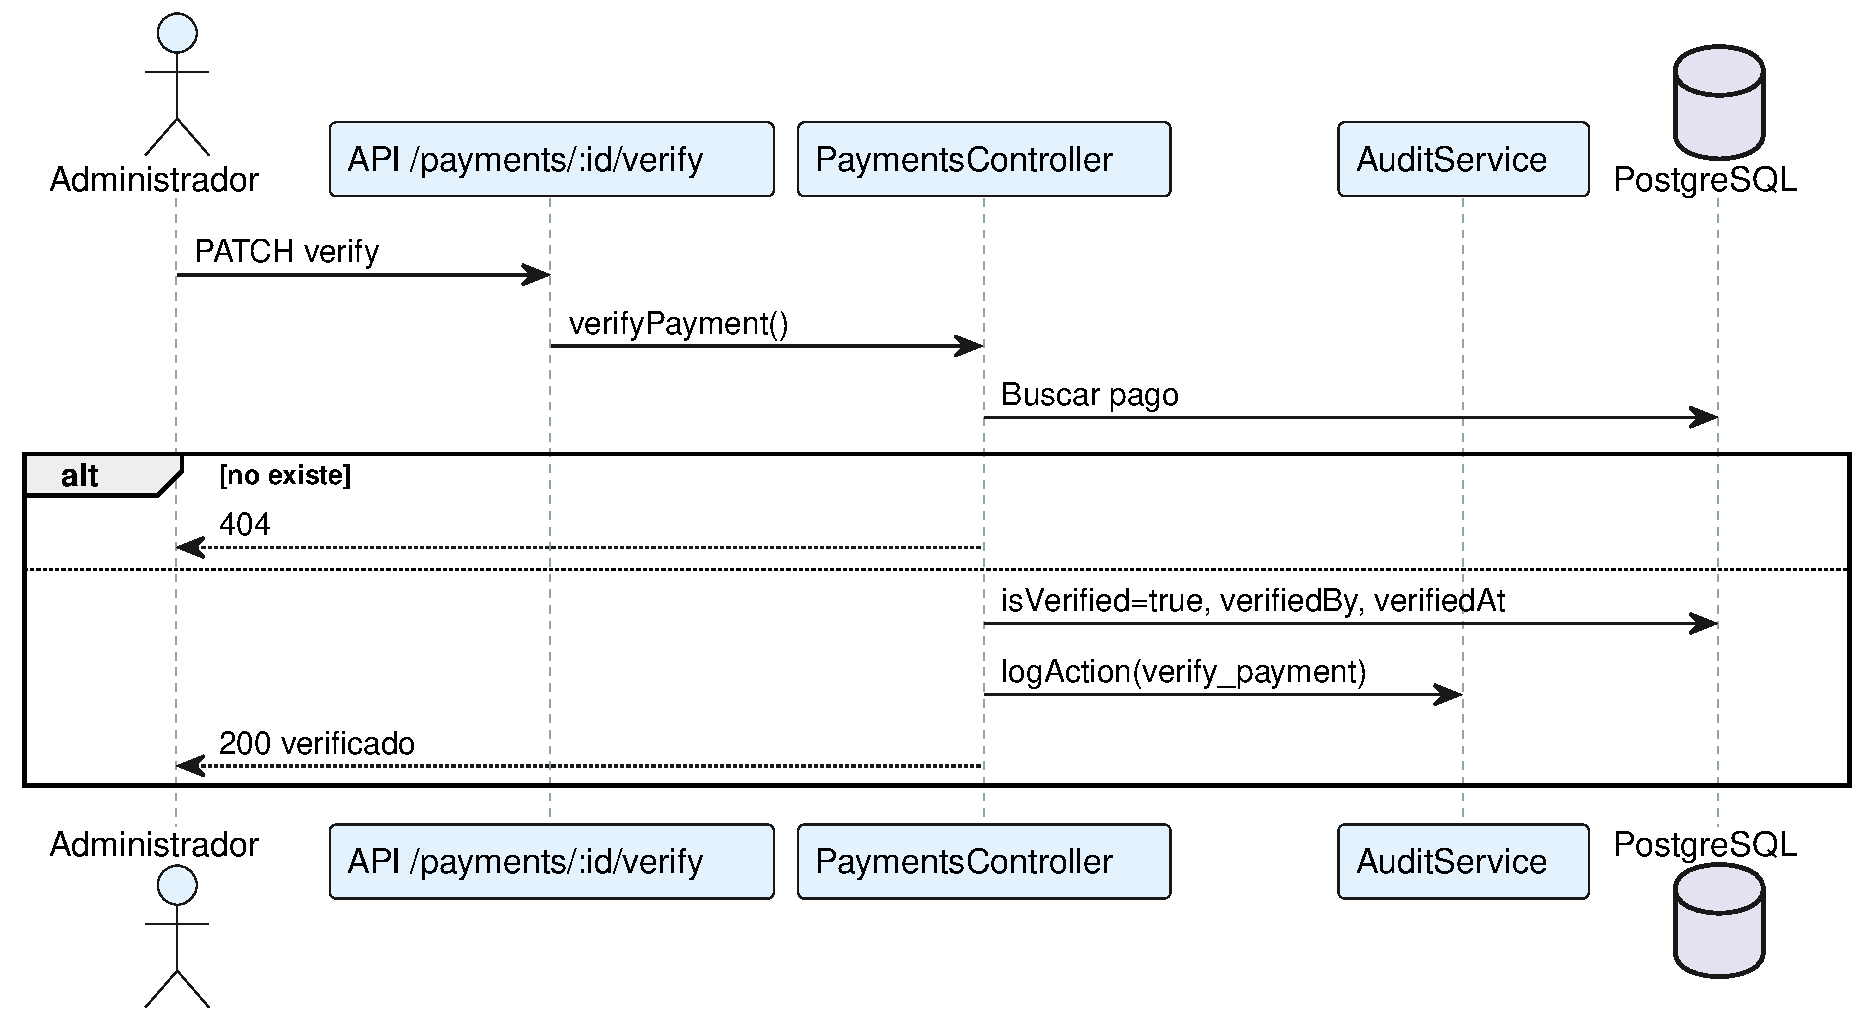
\includegraphics[width=\linewidth,height=0.42\textheight,keepaspectratio]{cu/cu12-seq.pdf}\caption{Diagrama de secuencia --- CU-12}\end{figure}
\begin{figure}[H]\centering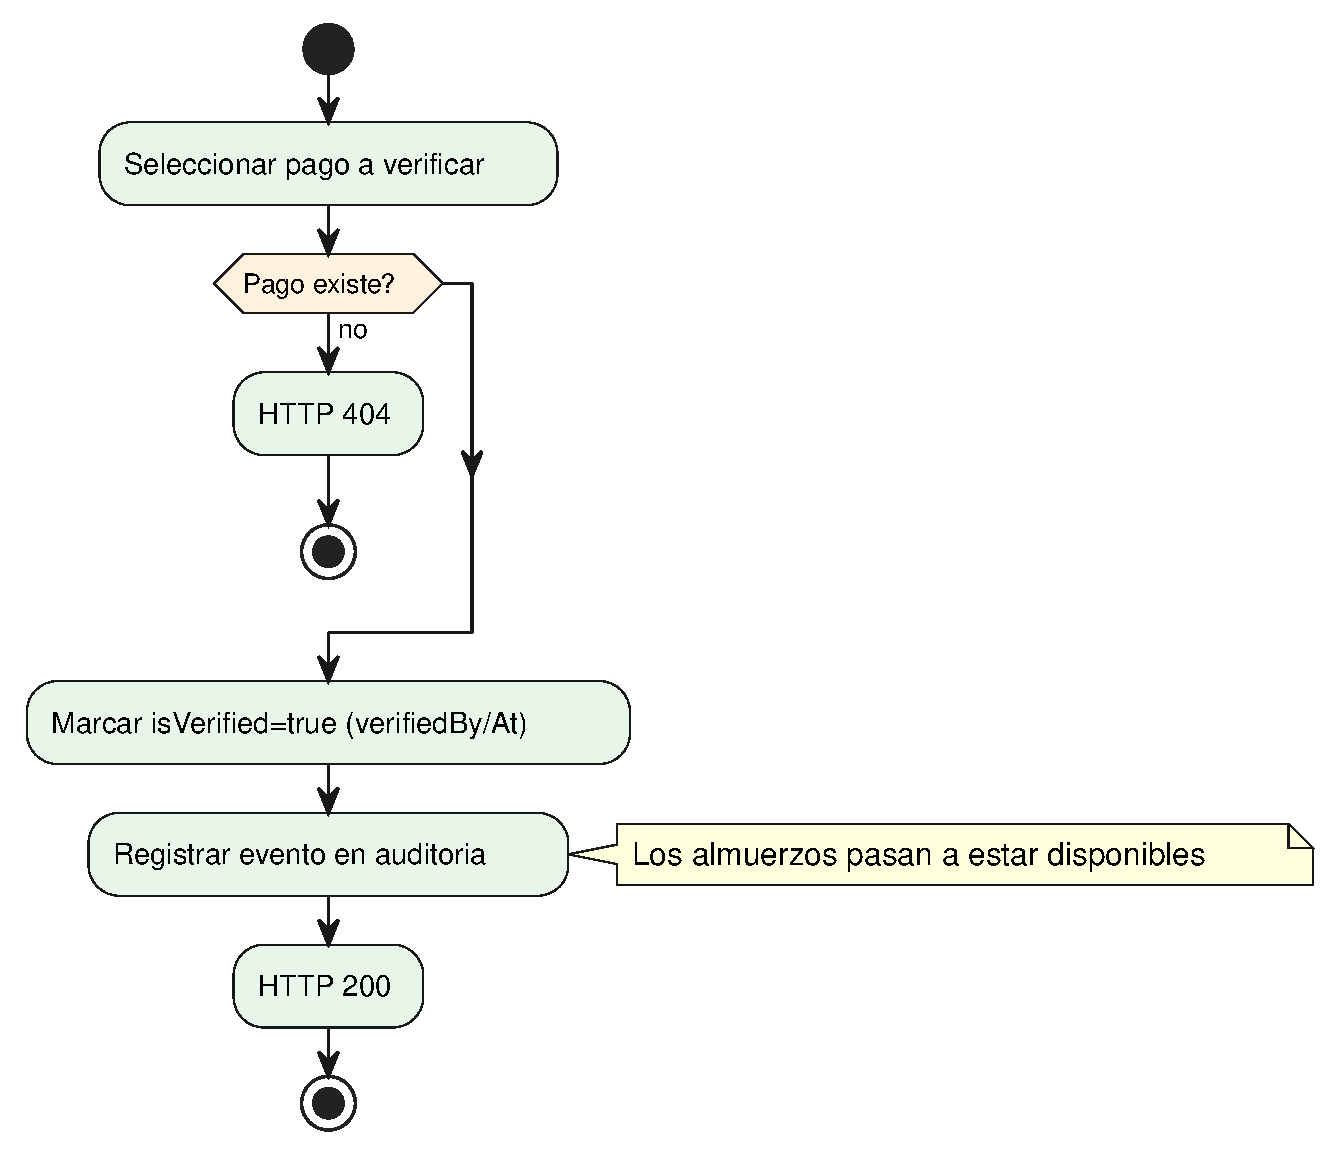
\includegraphics[width=\linewidth,height=0.46\textheight,keepaspectratio]{cu/cu12-act.pdf}\caption{Diagrama de actividades --- CU-12}\end{figure}

\subsection{CU-13 --- Calcular almuerzos por monto}

\noindent\textbf{Endpoint(s):} \texttt{POST /api/payments/calculate}\par\vspace{4pt}

\begin{table}[H]\centering\small
\caption{Ficha del caso de uso CU-13 --- Calcular almuerzos por monto}
\begin{tabularx}{\textwidth}{L{0.26\textwidth} X}
\toprule
\textbf{Campo} & \textbf{Descripcion} \\ \midrule
Objetivo del contexto & Permitir a un usuario autenticado conocer cuantos almuerzos corresponden a un monto dado, antes de registrar el pago. \\ \midrule
Precondiciones & El usuario debe estar autenticado. \\ \midrule
Condicion de exito & Se devuelve el numero de almuerzos y el residuo. \\ \midrule
Condicion de fracaso & El monto es invalido. \\ \midrule
Actores principales & Usuario autenticado \\ \midrule
Actores secundarios & - \\
\bottomrule\end{tabularx}\end{table}
\begin{table}[H]\centering\small
\caption{Flujo principal de CU-13}
\begin{tabularx}{\textwidth}{C{0.10\textwidth} X}
\toprule \textbf{Paso} & \textbf{Accion} \\ \midrule
1 & El usuario envia un monto. \\
2 & El sistema valida que el monto sea mayor o igual a 2000. \\
3 & El sistema calcula almuerzos=piso(monto/2000) y el residuo. \\
4 & El sistema responde 200 con el resultado. \\
\bottomrule\end{tabularx}\end{table}
\begin{table}[H]\centering\small
\caption{Extensiones (flujos alternativos) de CU-13}
\begin{tabularx}{\textwidth}{C{0.10\textwidth} X}
\toprule \textbf{Paso} & \textbf{Accion} \\ \midrule
2.1 & Monto menor a 2000 o no numerico $\rightarrow$ HTTP 400. \\
\bottomrule\end{tabularx}\end{table}
\begin{figure}[H]\centering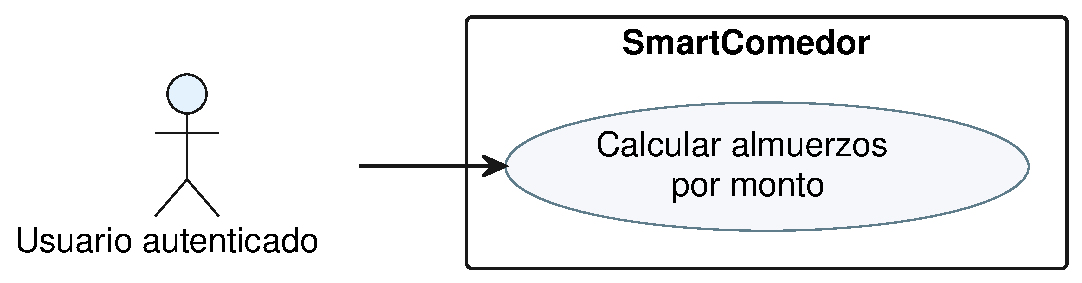
\includegraphics[width=\linewidth,height=0.30\textheight,keepaspectratio]{cu/cu13-uc.pdf}\caption{Diagrama de caso de uso --- CU-13}\end{figure}
\begin{figure}[H]\centering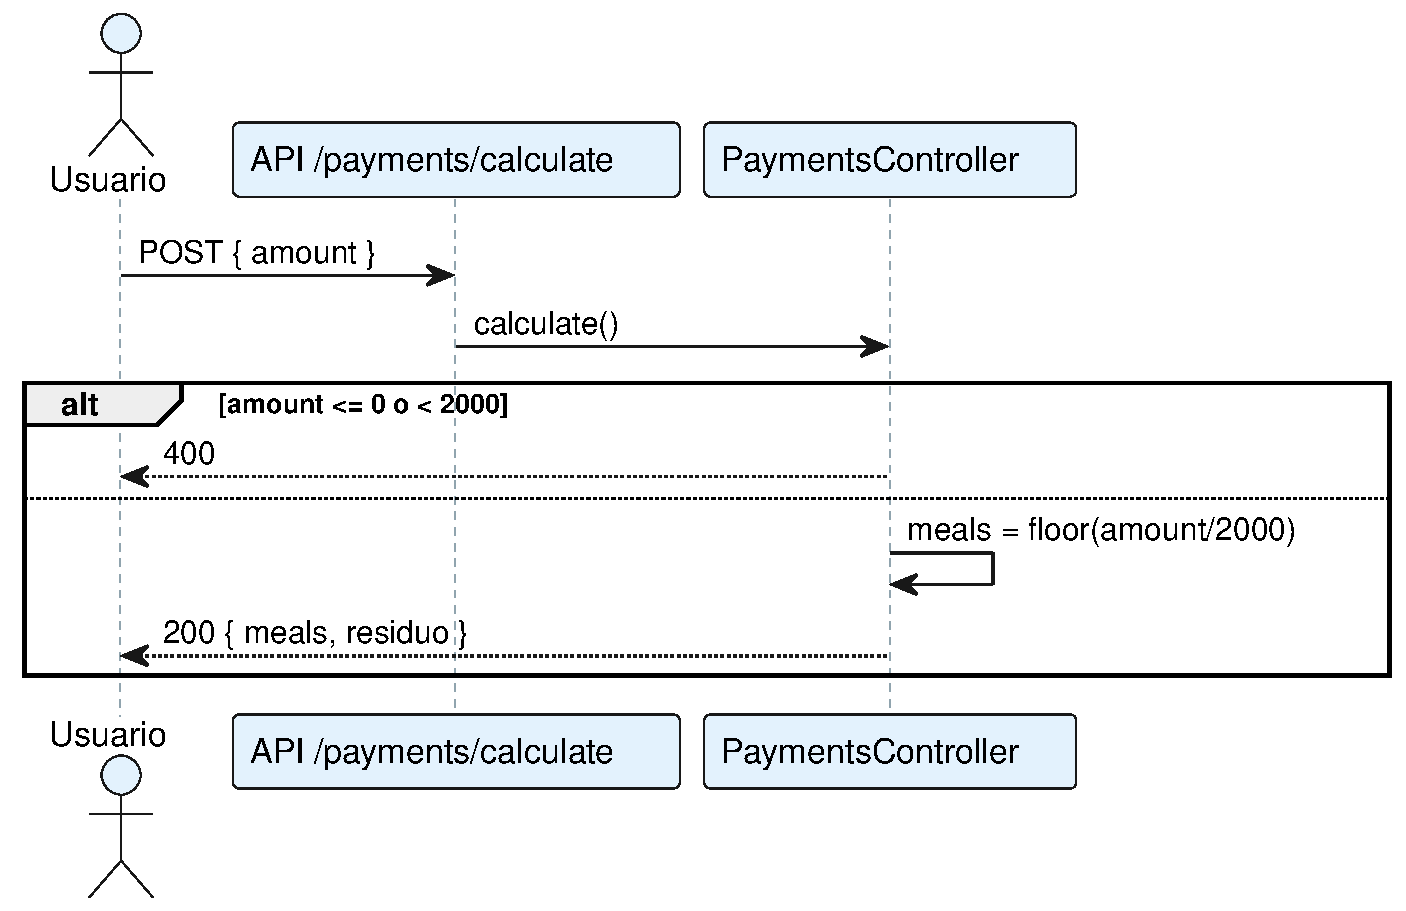
\includegraphics[width=\linewidth,height=0.42\textheight,keepaspectratio]{cu/cu13-seq.pdf}\caption{Diagrama de secuencia --- CU-13}\end{figure}
\begin{figure}[H]\centering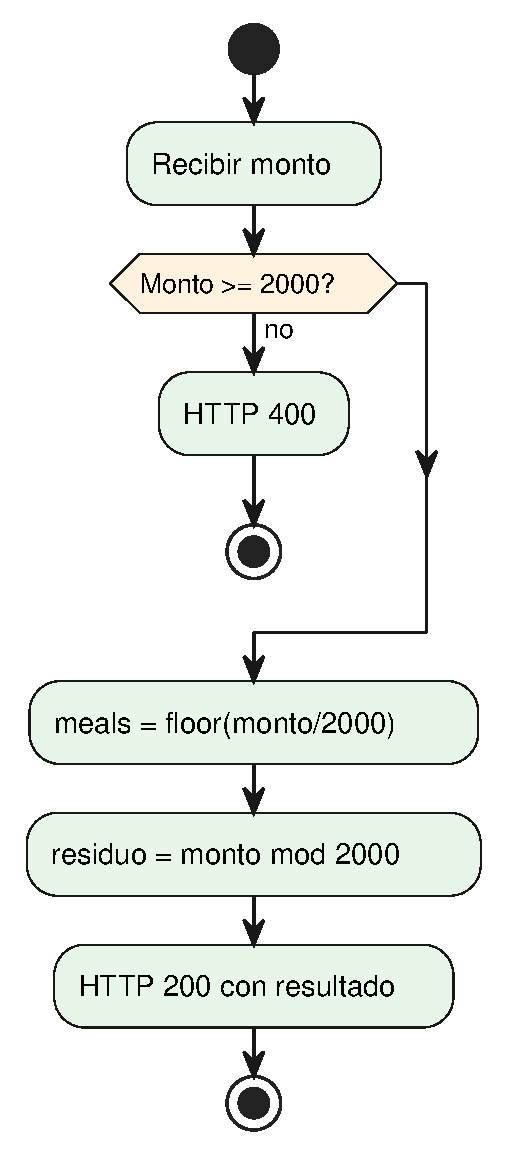
\includegraphics[width=\linewidth,height=0.46\textheight,keepaspectratio]{cu/cu13-act.pdf}\caption{Diagrama de actividades --- CU-13}\end{figure}

\subsection{CU-14 --- Registrar almuerzo}

\noindent\textbf{Endpoint(s):} \texttt{POST /api/meals}\par\vspace{4pt}

\begin{table}[H]\centering\small
\caption{Ficha del caso de uso CU-14 --- Registrar almuerzo}
\begin{tabularx}{\textwidth}{L{0.26\textwidth} X}
\toprule
\textbf{Campo} & \textbf{Descripcion} \\ \midrule
Objetivo del contexto & Permitir al supervisor registrar el consumo de almuerzo de un estudiante validando todas las reglas de elegibilidad del dia. \\ \midrule
Precondiciones & El supervisor debe estar autenticado; el estudiante debe estar activo y tener almuerzos. \\ \midrule
Condicion de exito & Se registra la asistencia, se descuenta un almuerzo y se deja bitacora. \\ \midrule
Condicion de fracaso & El estudiante no cumple alguna regla (inactivo, dia no permitido, ya comio, sin saldo). \\ \midrule
Actores principales & Supervisor \\ \midrule
Actores secundarios & Servicios de bitacora y auditoria \\
\bottomrule\end{tabularx}\end{table}
\begin{table}[H]\centering\small
\caption{Flujo principal de CU-14}
\begin{tabularx}{\textwidth}{C{0.10\textwidth} X}
\toprule \textbf{Paso} & \textbf{Accion} \\ \midrule
1 & El supervisor busca al estudiante por QR, cedula o UID. \\
2 & El sistema valida que exista y este activo. \\
3 & El sistema valida el dia autorizado y que no haya comido hoy. \\
4 & El sistema valida que tenga almuerzos disponibles. \\
5 & El sistema registra la asistencia e incrementa mealsUsed. \\
6 & El sistema registra la bitacora y la auditoria, y responde 201. \\
\bottomrule\end{tabularx}\end{table}
\begin{table}[H]\centering\small
\caption{Extensiones (flujos alternativos) de CU-14}
\begin{tabularx}{\textwidth}{C{0.10\textwidth} X}
\toprule \textbf{Paso} & \textbf{Accion} \\ \midrule
2.1 & Estudiante inexistente $\rightarrow$ 404; inactivo $\rightarrow$ 400. \\
3.1 & Dia no autorizado o ya comio hoy $\rightarrow$ 400. \\
4.1 & Sin almuerzos disponibles $\rightarrow$ 400. \\
\bottomrule\end{tabularx}\end{table}
\begin{figure}[H]\centering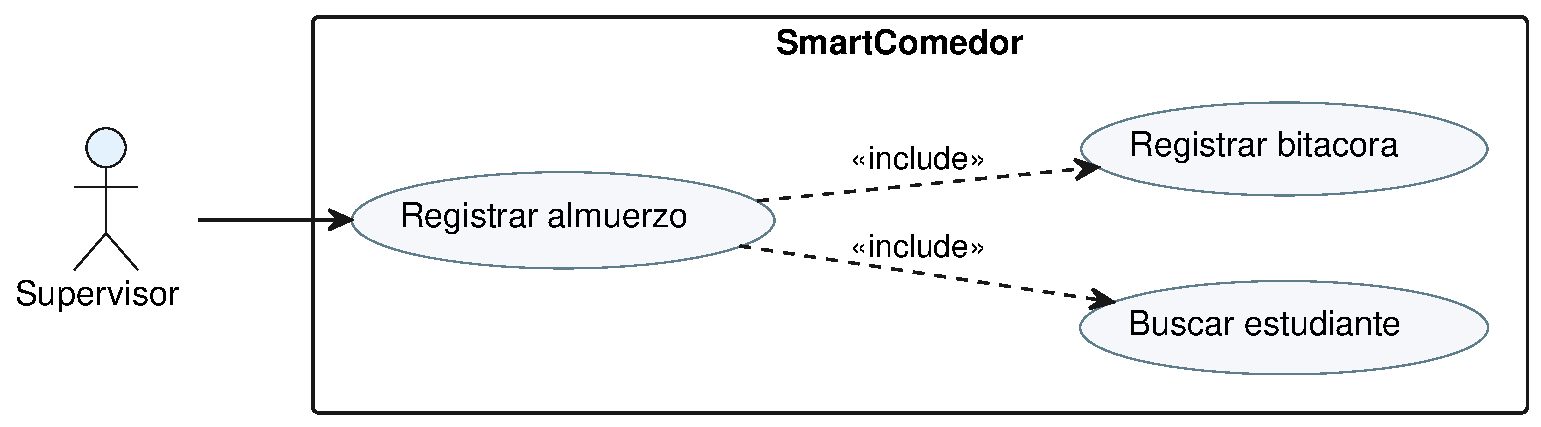
\includegraphics[width=\linewidth,height=0.30\textheight,keepaspectratio]{cu/cu14-uc.pdf}\caption{Diagrama de caso de uso --- CU-14}\end{figure}
\begin{figure}[H]\centering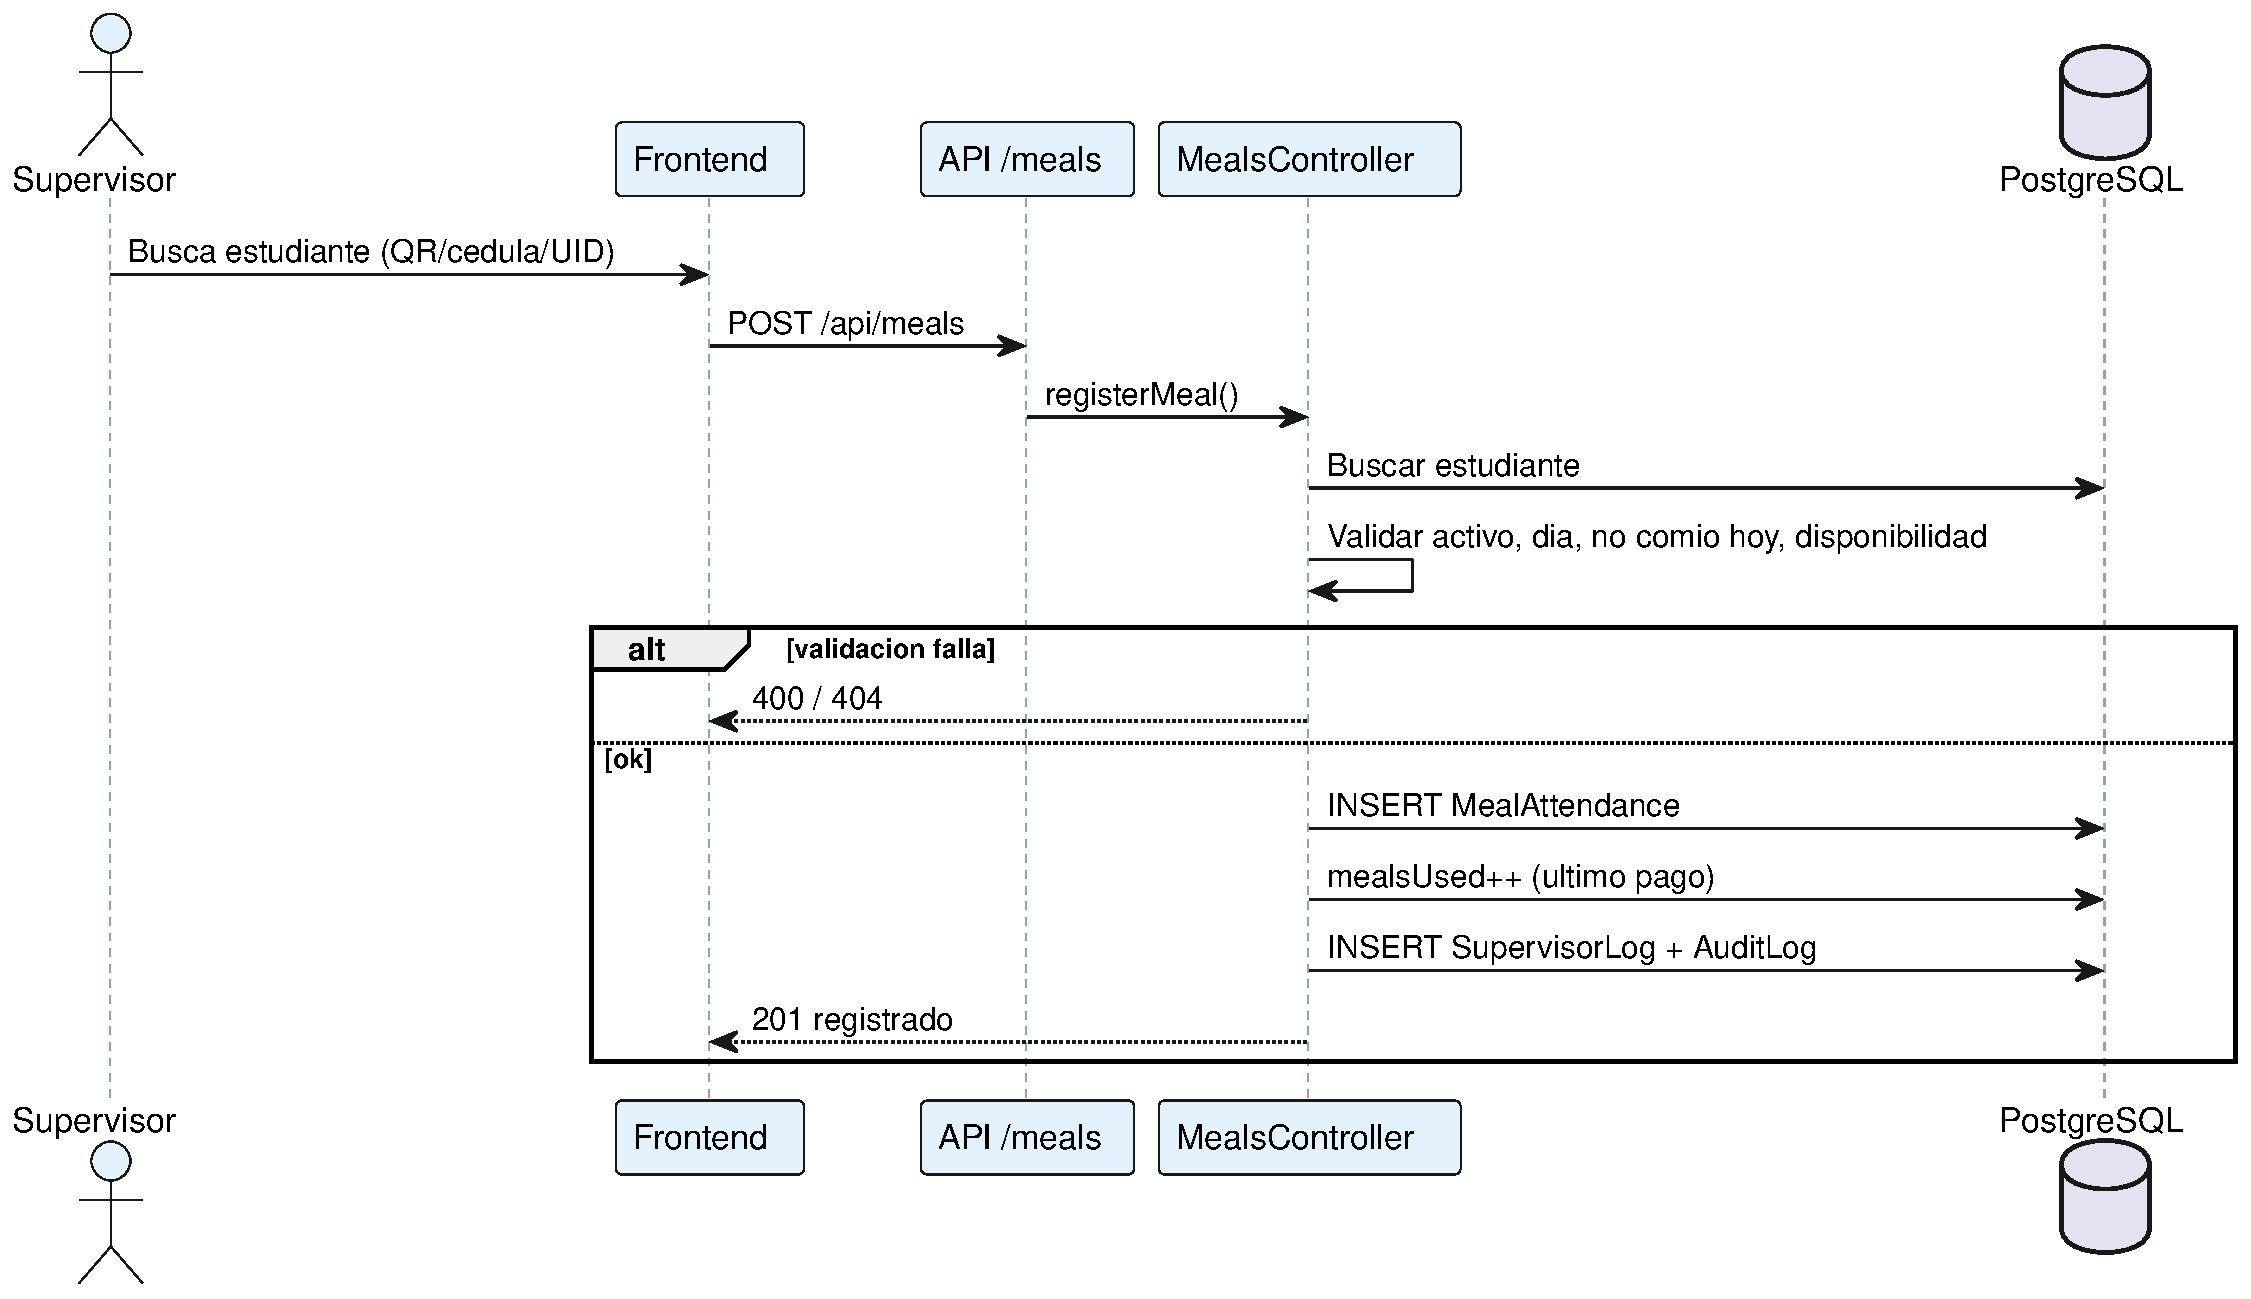
\includegraphics[width=\linewidth,height=0.42\textheight,keepaspectratio]{cu/cu14-seq.pdf}\caption{Diagrama de secuencia --- CU-14}\end{figure}
\begin{figure}[H]\centering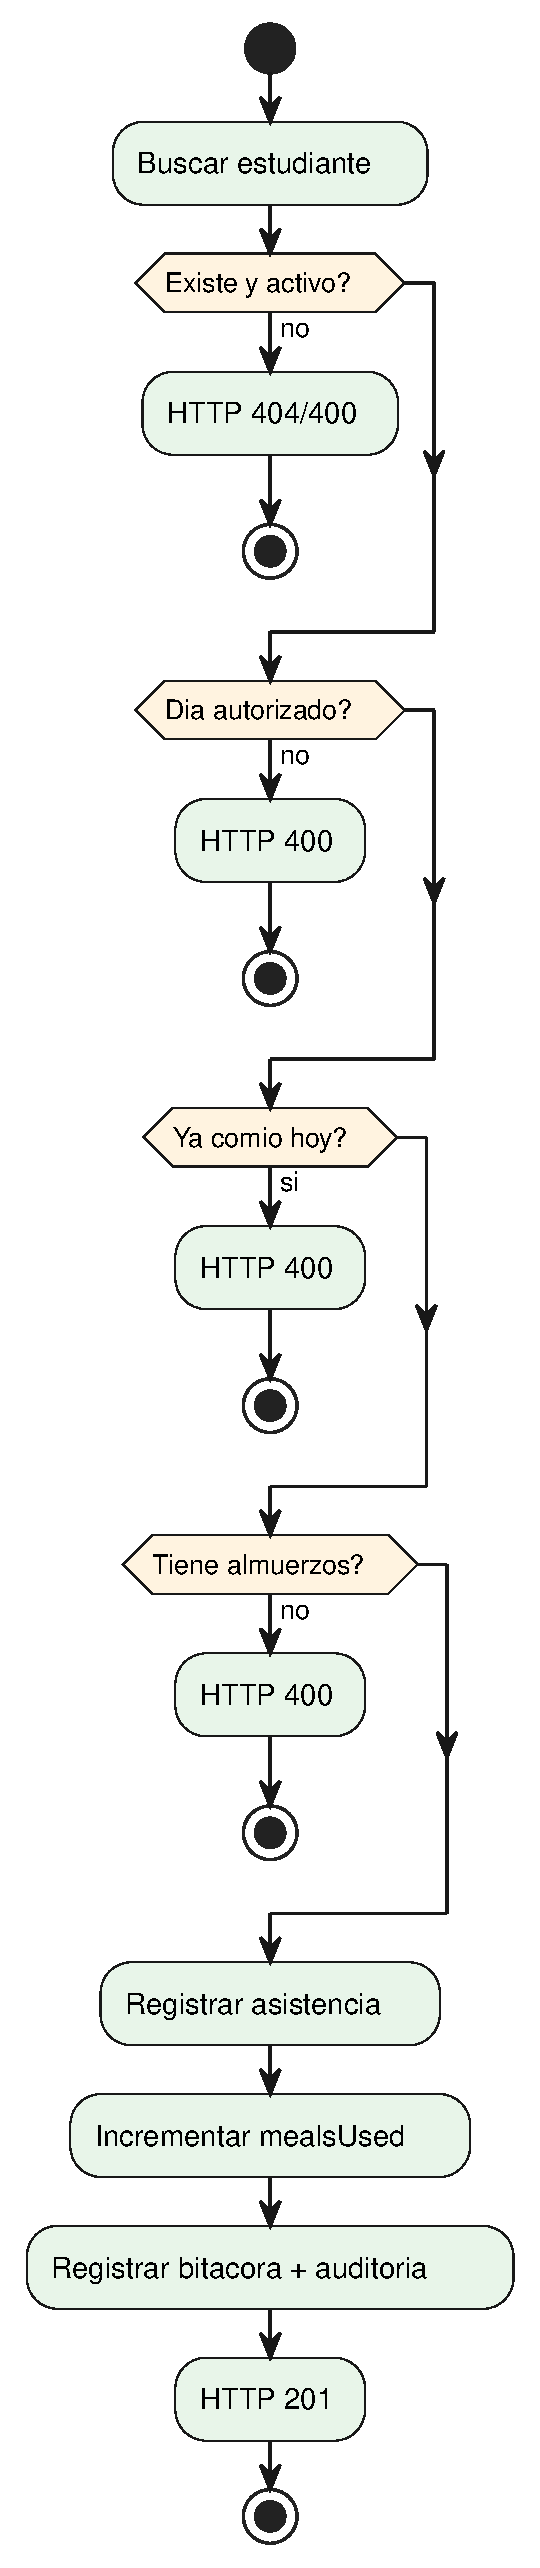
\includegraphics[width=\linewidth,height=0.46\textheight,keepaspectratio]{cu/cu14-act.pdf}\caption{Diagrama de actividades --- CU-14}\end{figure}

\subsection{CU-15 --- Consultar historial y asistencia del dia}

\noindent\textbf{Endpoint(s):} \texttt{GET /api/meals/history, GET /api/meals/today}\par\vspace{4pt}

\begin{table}[H]\centering\small
\caption{Ficha del caso de uso CU-15 --- Consultar historial y asistencia del dia}
\begin{tabularx}{\textwidth}{L{0.26\textwidth} X}
\toprule
\textbf{Campo} & \textbf{Descripcion} \\ \midrule
Objetivo del contexto & Permitir a los usuarios autorizados consultar el historial de almuerzos y la asistencia del dia. \\ \midrule
Precondiciones & El usuario debe estar autenticado. \\ \midrule
Condicion de exito & Se devuelven los registros segun los filtros. \\ \midrule
Condicion de fracaso & Parametros de filtro invalidos. \\ \midrule
Actores principales & Usuario autenticado \\ \midrule
Actores secundarios & Base de datos \\
\bottomrule\end{tabularx}\end{table}
\begin{table}[H]\centering\small
\caption{Flujo principal de CU-15}
\begin{tabularx}{\textwidth}{C{0.10\textwidth} X}
\toprule \textbf{Paso} & \textbf{Accion} \\ \midrule
1 & El usuario elige consultar historial o asistencia del dia. \\
2 & El usuario aplica filtros (estudiante, rango de fechas). \\
3 & El sistema consulta las asistencias correspondientes. \\
4 & El sistema responde 200 con los resultados. \\
\bottomrule\end{tabularx}\end{table}
\begin{table}[H]\centering\small
\caption{Extensiones (flujos alternativos) de CU-15}
\begin{tabularx}{\textwidth}{C{0.10\textwidth} X}
\toprule \textbf{Paso} & \textbf{Accion} \\ \midrule
2.1 & Filtros invalidos $\rightarrow$ HTTP 400. \\
\bottomrule\end{tabularx}\end{table}
\begin{figure}[H]\centering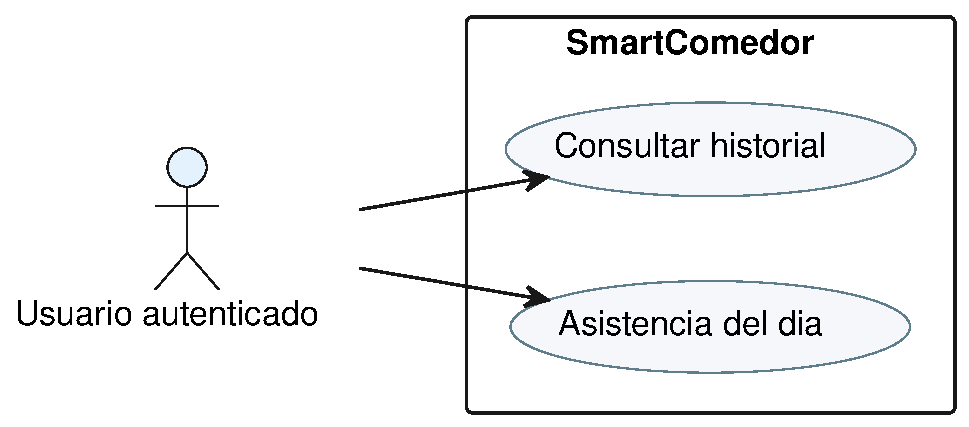
\includegraphics[width=\linewidth,height=0.30\textheight,keepaspectratio]{cu/cu15-uc.pdf}\caption{Diagrama de caso de uso --- CU-15}\end{figure}
\begin{figure}[H]\centering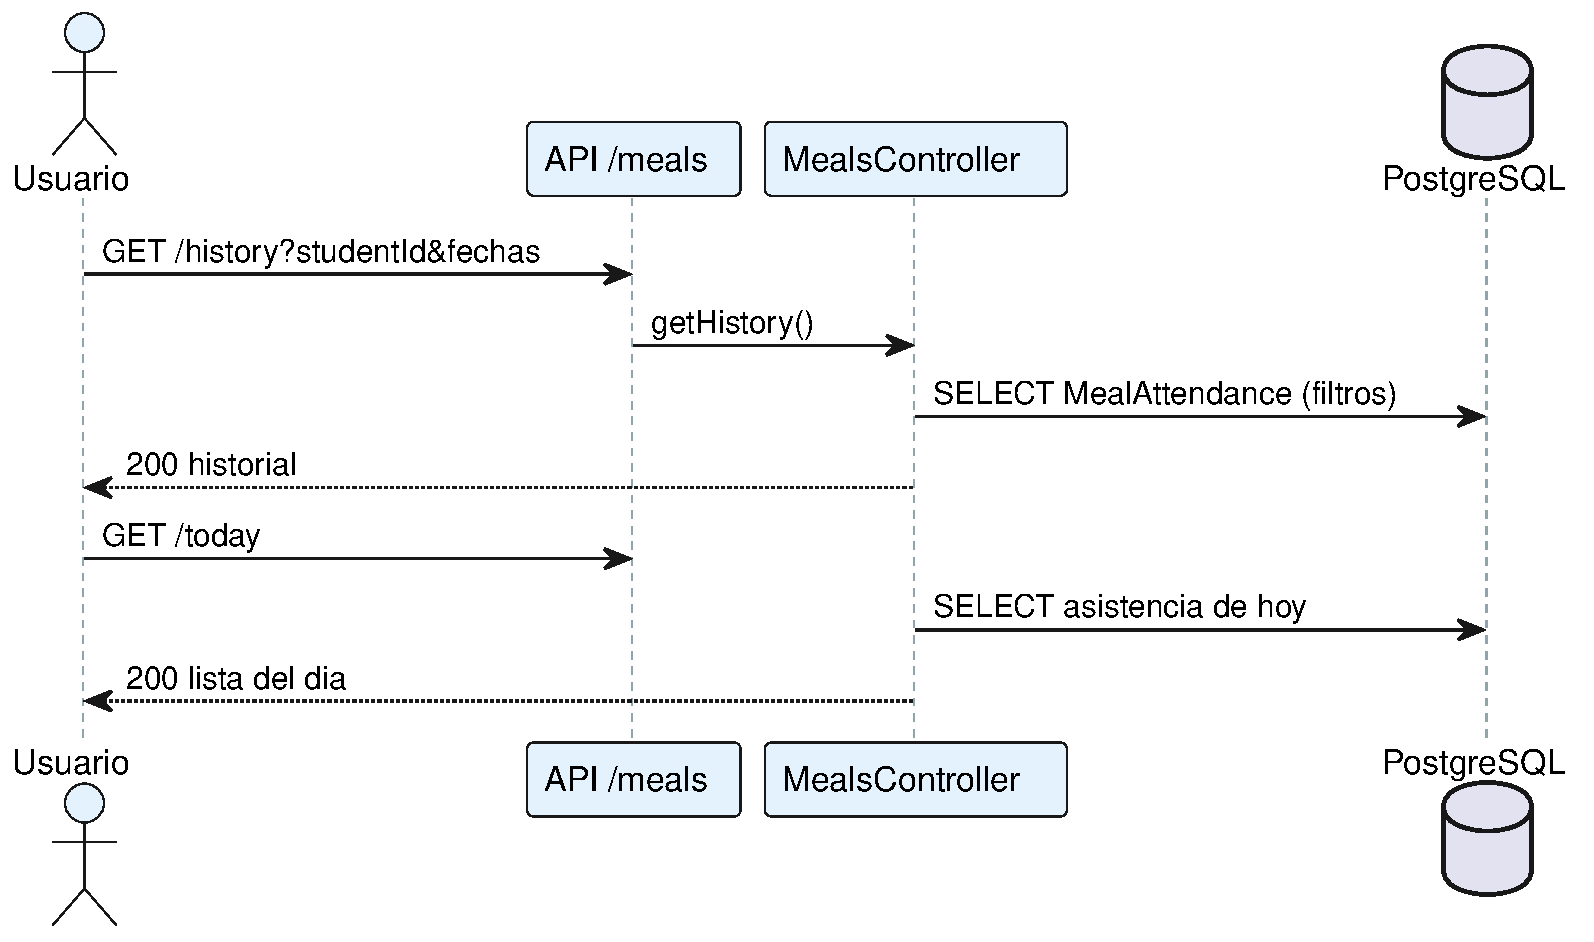
\includegraphics[width=\linewidth,height=0.42\textheight,keepaspectratio]{cu/cu15-seq.pdf}\caption{Diagrama de secuencia --- CU-15}\end{figure}
\begin{figure}[H]\centering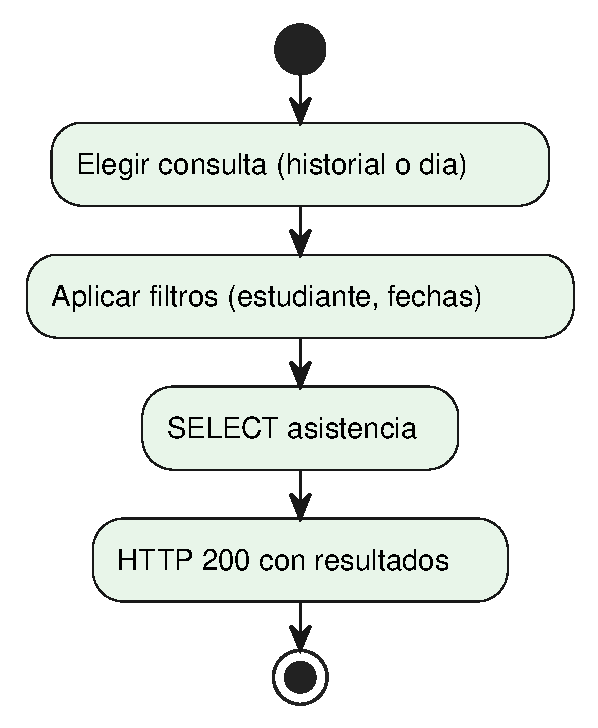
\includegraphics[width=\linewidth,height=0.46\textheight,keepaspectratio]{cu/cu15-act.pdf}\caption{Diagrama de actividades --- CU-15}\end{figure}

\subsection{CU-16 --- Consultar analitica del tablero}

\noindent\textbf{Endpoint(s):} \texttt{GET /api/meals/analytics}\par\vspace{4pt}

\begin{table}[H]\centering\small
\caption{Ficha del caso de uso CU-16 --- Consultar analitica del tablero}
\begin{tabularx}{\textwidth}{L{0.26\textwidth} X}
\toprule
\textbf{Campo} & \textbf{Descripcion} \\ \midrule
Objetivo del contexto & Proveer indicadores agregados (KPIs) del servicio de comedor para la toma de decisiones. \\ \midrule
Precondiciones & El usuario debe tener rol admin o auditor. \\ \midrule
Condicion de exito & Se devuelven las metricas agregadas. \\ \midrule
Condicion de fracaso & Sin autorizacion. \\ \midrule
Actores principales & Administrador, Auditor externo \\ \midrule
Actores secundarios & Base de datos \\
\bottomrule\end{tabularx}\end{table}
\begin{table}[H]\centering\small
\caption{Flujo principal de CU-16}
\begin{tabularx}{\textwidth}{C{0.10\textwidth} X}
\toprule \textbf{Paso} & \textbf{Accion} \\ \midrule
1 & El usuario solicita la analitica del tablero. \\
2 & El sistema ejecuta las agregaciones (conteos y totales). \\
3 & El sistema construye la respuesta con los KPIs. \\
4 & El sistema responde 200. \\
\bottomrule\end{tabularx}\end{table}
\begin{table}[H]\centering\small
\caption{Extensiones (flujos alternativos) de CU-16}
\begin{tabularx}{\textwidth}{C{0.10\textwidth} X}
\toprule \textbf{Paso} & \textbf{Accion} \\ \midrule
1.1 & Rol no autorizado $\rightarrow$ HTTP 403. \\
\bottomrule\end{tabularx}\end{table}
\begin{figure}[H]\centering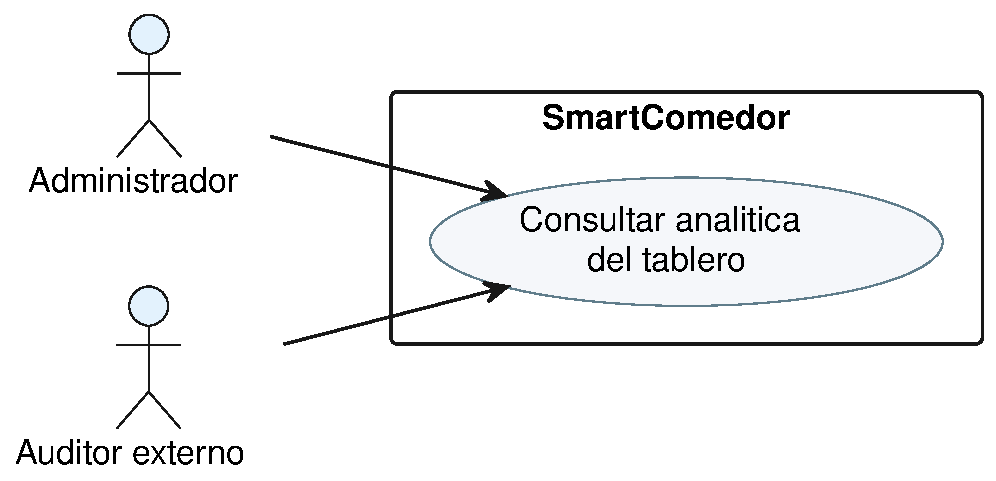
\includegraphics[width=\linewidth,height=0.30\textheight,keepaspectratio]{cu/cu16-uc.pdf}\caption{Diagrama de caso de uso --- CU-16}\end{figure}
\begin{figure}[H]\centering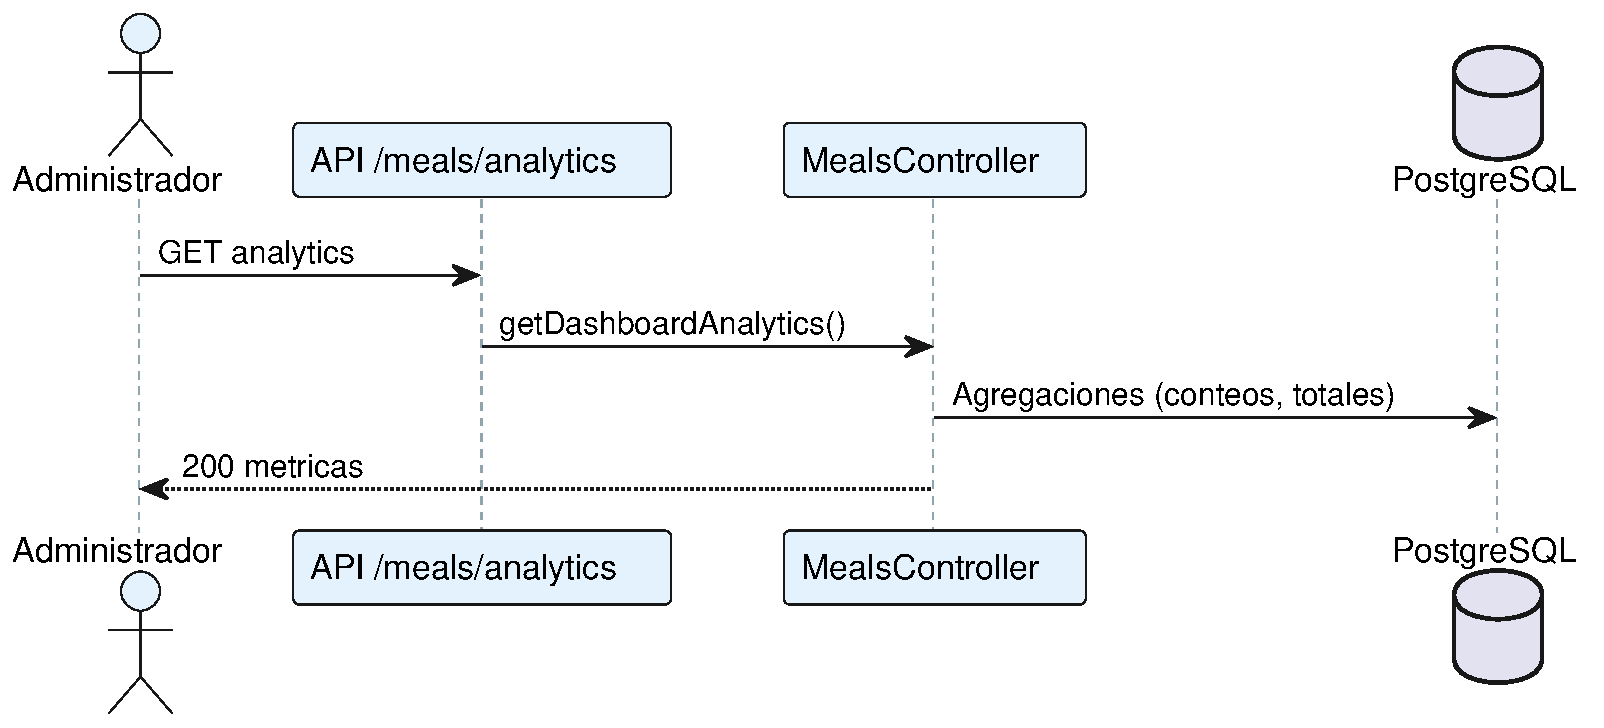
\includegraphics[width=\linewidth,height=0.42\textheight,keepaspectratio]{cu/cu16-seq.pdf}\caption{Diagrama de secuencia --- CU-16}\end{figure}
\begin{figure}[H]\centering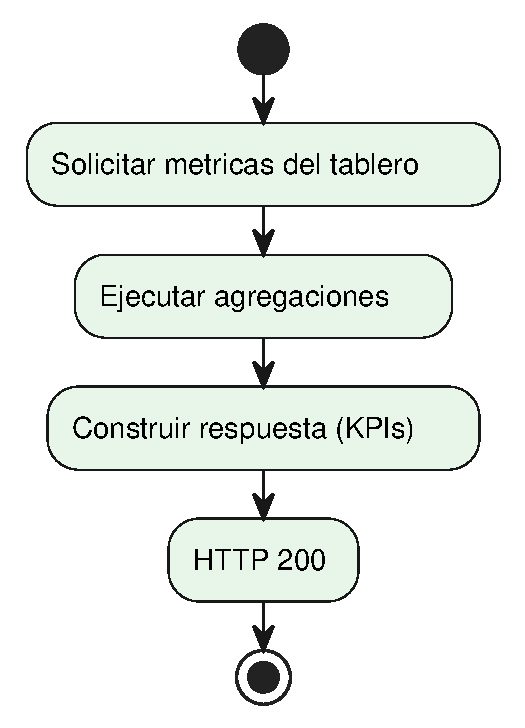
\includegraphics[width=\linewidth,height=0.46\textheight,keepaspectratio]{cu/cu16-act.pdf}\caption{Diagrama de actividades --- CU-16}\end{figure}

\subsection{CU-17 --- Gestionar ciclos y cierre automatico}

\noindent\textbf{Endpoint(s):} \texttt{GET/POST/PUT /api/cycles + tarea programada}\par\vspace{4pt}

\begin{table}[H]\centering\small
\caption{Ficha del caso de uso CU-17 --- Gestionar ciclos y cierre automatico}
\begin{tabularx}{\textwidth}{L{0.26\textwidth} X}
\toprule
\textbf{Campo} & \textbf{Descripcion} \\ \midrule
Objetivo del contexto & Administrar los periodos del servicio y cerrar automaticamente los ciclos vencidos solicitando revalidacion documental. \\ \midrule
Precondiciones & Debe existir al menos un ciclo configurado. \\ \midrule
Condicion de exito & Los ciclos vencidos se cierran y los estudiantes quedan marcados para revalidacion. \\ \midrule
Condicion de fracaso & No hay ciclos vencidos por procesar. \\ \midrule
Actores principales & Administrador, Sistema (cron) \\ \midrule
Actores secundarios & Servicio de automatizacion de ciclos \\
\bottomrule\end{tabularx}\end{table}
\begin{table}[H]\centering\small
\caption{Flujo principal de CU-17}
\begin{tabularx}{\textwidth}{C{0.10\textwidth} X}
\toprule \textbf{Paso} & \textbf{Accion} \\ \midrule
1 & El administrador crea o cierra ciclos manualmente. \\
2 & Una tarea programada se ejecuta periodicamente. \\
3 & El sistema busca ciclos activos cuya fecha de fin ya paso. \\
4 & El sistema cierra cada ciclo y marca a los estudiantes para revalidacion. \\
\bottomrule\end{tabularx}\end{table}
\begin{table}[H]\centering\small
\caption{Extensiones (flujos alternativos) de CU-17}
\begin{tabularx}{\textwidth}{C{0.10\textwidth} X}
\toprule \textbf{Paso} & \textbf{Accion} \\ \midrule
3.1 & Si no hay ciclos vencidos, la tarea finaliza sin cambios. \\
\bottomrule\end{tabularx}\end{table}
\begin{figure}[H]\centering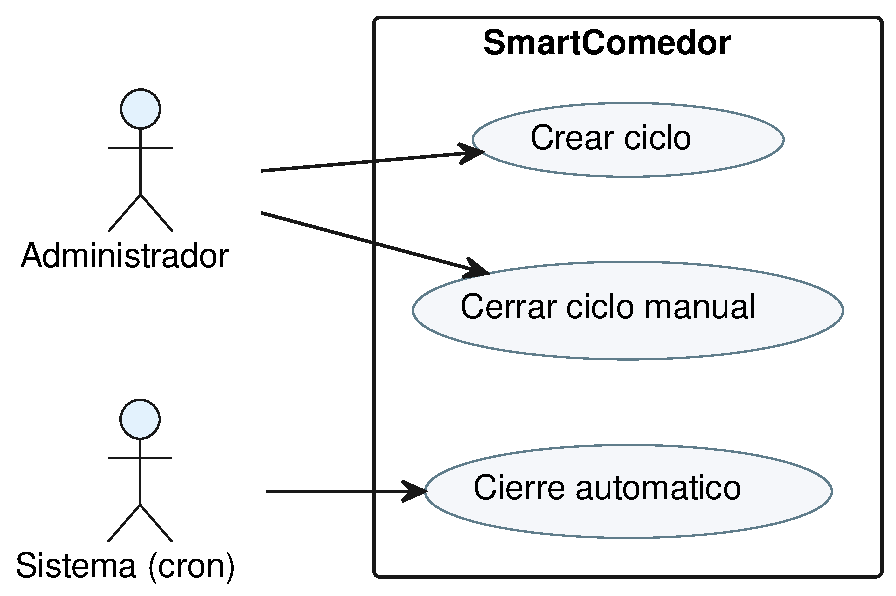
\includegraphics[width=\linewidth,height=0.30\textheight,keepaspectratio]{cu/cu17-uc.pdf}\caption{Diagrama de caso de uso --- CU-17}\end{figure}
\begin{figure}[H]\centering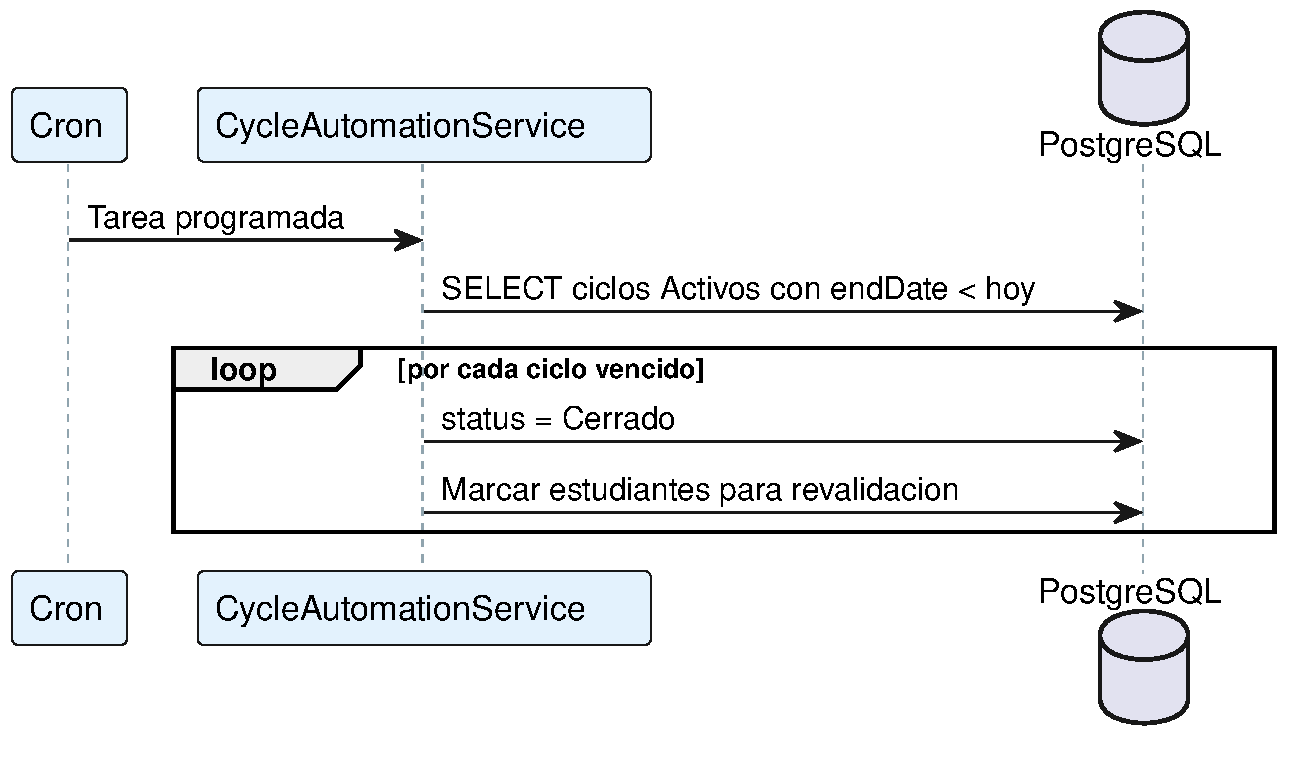
\includegraphics[width=\linewidth,height=0.42\textheight,keepaspectratio]{cu/cu17-seq.pdf}\caption{Diagrama de secuencia --- CU-17}\end{figure}
\begin{figure}[H]\centering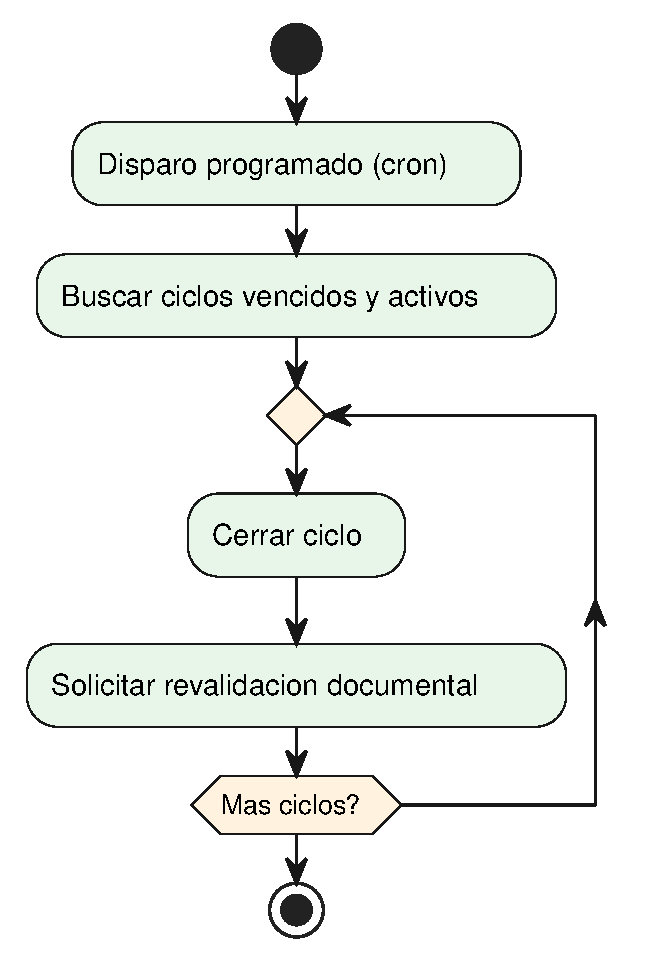
\includegraphics[width=\linewidth,height=0.46\textheight,keepaspectratio]{cu/cu17-act.pdf}\caption{Diagrama de actividades --- CU-17}\end{figure}

\subsection{CU-18 --- Calificar servicio}

\noindent\textbf{Endpoint(s):} \texttt{POST /api/ratings}\par\vspace{4pt}

\begin{table}[H]\centering\small
\caption{Ficha del caso de uso CU-18 --- Calificar servicio}
\begin{tabularx}{\textwidth}{L{0.26\textwidth} X}
\toprule
\textbf{Campo} & \textbf{Descripcion} \\ \midrule
Objetivo del contexto & Permitir al estudiante calificar el servicio del comedor con una puntuacion y un comentario opcional. \\ \midrule
Precondiciones & El estudiante debe estar autenticado. \\ \midrule
Condicion de exito & Se registra la calificacion y se actualiza el promedio. \\ \midrule
Condicion de fracaso & Usuario no autenticado. \\ \midrule
Actores principales & Estudiante \\ \midrule
Actores secundarios & Base de datos \\
\bottomrule\end{tabularx}\end{table}
\begin{table}[H]\centering\small
\caption{Flujo principal de CU-18}
\begin{tabularx}{\textwidth}{C{0.10\textwidth} X}
\toprule \textbf{Paso} & \textbf{Accion} \\ \midrule
1 & El estudiante selecciona una puntuacion de 1 a 5 estrellas. \\
2 & El estudiante agrega un comentario opcional. \\
3 & El sistema registra la calificacion. \\
4 & El sistema responde 201. \\
\bottomrule\end{tabularx}\end{table}
\begin{table}[H]\centering\small
\caption{Extensiones (flujos alternativos) de CU-18}
\begin{tabularx}{\textwidth}{C{0.10\textwidth} X}
\toprule \textbf{Paso} & \textbf{Accion} \\ \midrule
3.1 & Usuario no autenticado $\rightarrow$ HTTP 401. \\
\bottomrule\end{tabularx}\end{table}
\begin{figure}[H]\centering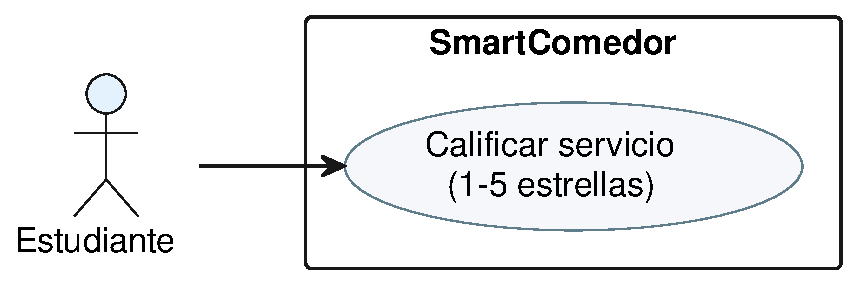
\includegraphics[width=\linewidth,height=0.30\textheight,keepaspectratio]{cu/cu18-uc.pdf}\caption{Diagrama de caso de uso --- CU-18}\end{figure}
\begin{figure}[H]\centering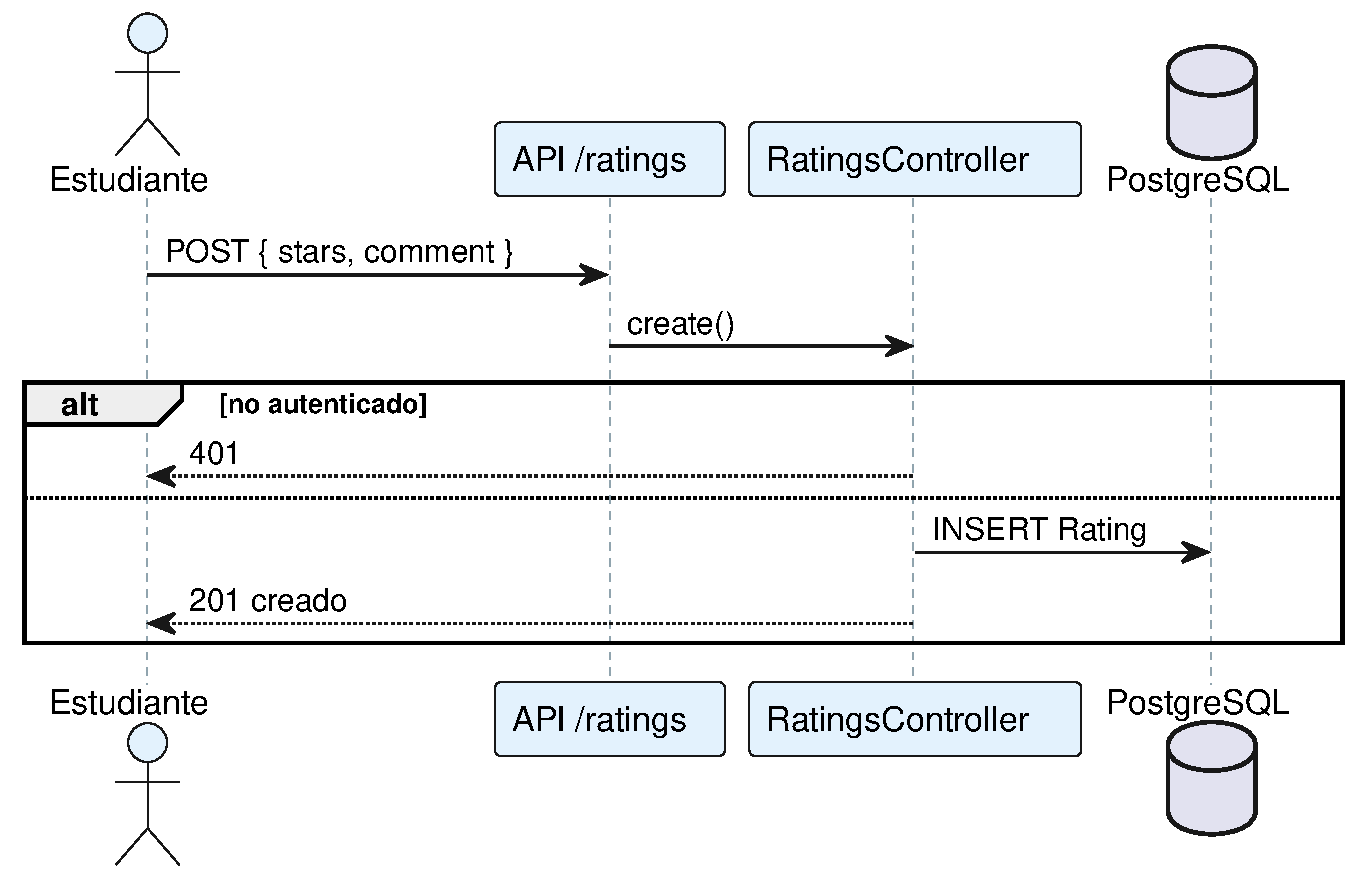
\includegraphics[width=\linewidth,height=0.42\textheight,keepaspectratio]{cu/cu18-seq.pdf}\caption{Diagrama de secuencia --- CU-18}\end{figure}
\begin{figure}[H]\centering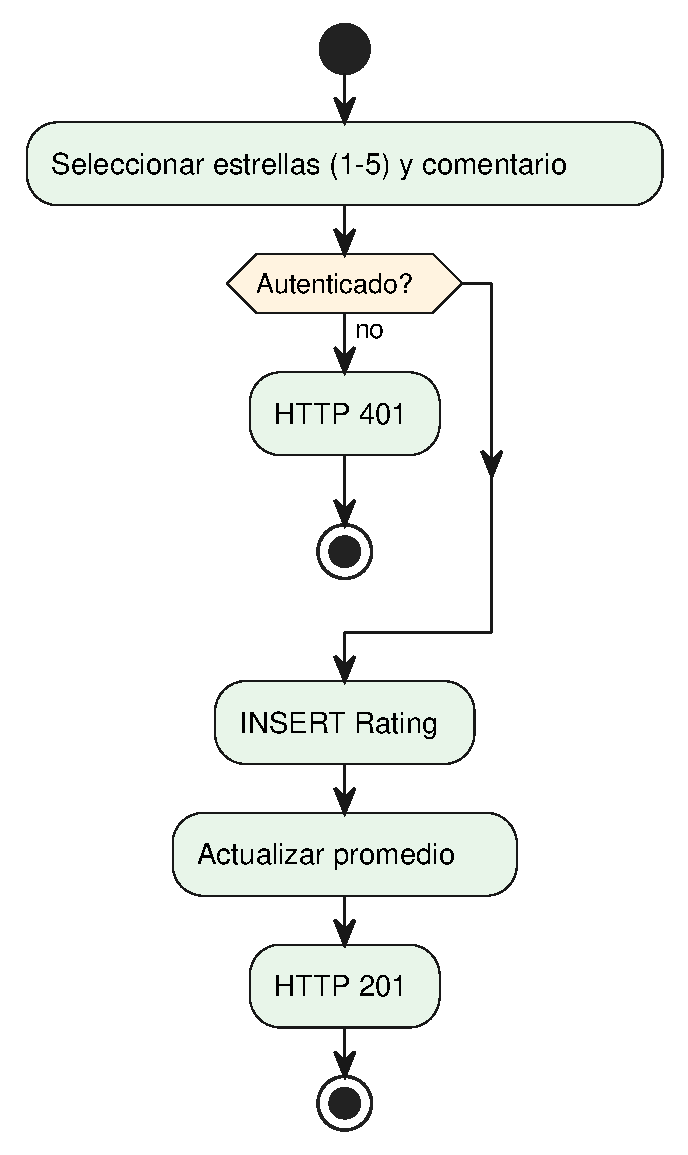
\includegraphics[width=\linewidth,height=0.46\textheight,keepaspectratio]{cu/cu18-act.pdf}\caption{Diagrama de actividades --- CU-18}\end{figure}

\subsection{CU-19 --- Enviar y responder quejas}

\noindent\textbf{Endpoint(s):} \texttt{POST /api/complaints, POST /api/complaints/:id/respond}\par\vspace{4pt}

\begin{table}[H]\centering\small
\caption{Ficha del caso de uso CU-19 --- Enviar y responder quejas}
\begin{tabularx}{\textwidth}{L{0.26\textwidth} X}
\toprule
\textbf{Campo} & \textbf{Descripcion} \\ \midrule
Objetivo del contexto & Permitir al estudiante enviar quejas, sugerencias o comentarios (anonimos o no) y al administrador responderlas. \\ \midrule
Precondiciones & El estudiante debe estar autenticado para enviar; el administrador para responder. \\ \midrule
Condicion de exito & Se registra la queja y, en su caso, la respuesta del administrador. \\ \midrule
Condicion de fracaso & Datos invalidos. \\ \midrule
Actores principales & Estudiante, Administrador \\ \midrule
Actores secundarios & Base de datos \\
\bottomrule\end{tabularx}\end{table}
\begin{table}[H]\centering\small
\caption{Flujo principal de CU-19}
\begin{tabularx}{\textwidth}{C{0.10\textwidth} X}
\toprule \textbf{Paso} & \textbf{Accion} \\ \midrule
1 & El estudiante crea una queja/sugerencia/comentario. \\
2 & Si es anonima, no se asocia al estudiante. \\
3 & El sistema registra la queja. \\
4 & El administrador responde y la marca como resuelta. \\
\bottomrule\end{tabularx}\end{table}
\begin{table}[H]\centering\small
\caption{Extensiones (flujos alternativos) de CU-19}
\begin{tabularx}{\textwidth}{C{0.10\textwidth} X}
\toprule \textbf{Paso} & \textbf{Accion} \\ \midrule
1.1 & Contenido vacio $\rightarrow$ HTTP 400. \\
\bottomrule\end{tabularx}\end{table}
\begin{figure}[H]\centering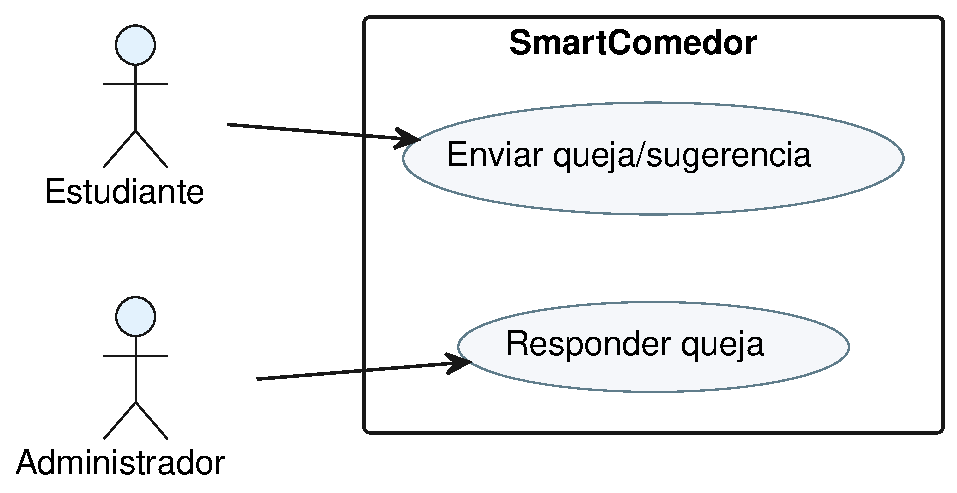
\includegraphics[width=\linewidth,height=0.30\textheight,keepaspectratio]{cu/cu19-uc.pdf}\caption{Diagrama de caso de uso --- CU-19}\end{figure}
\begin{figure}[H]\centering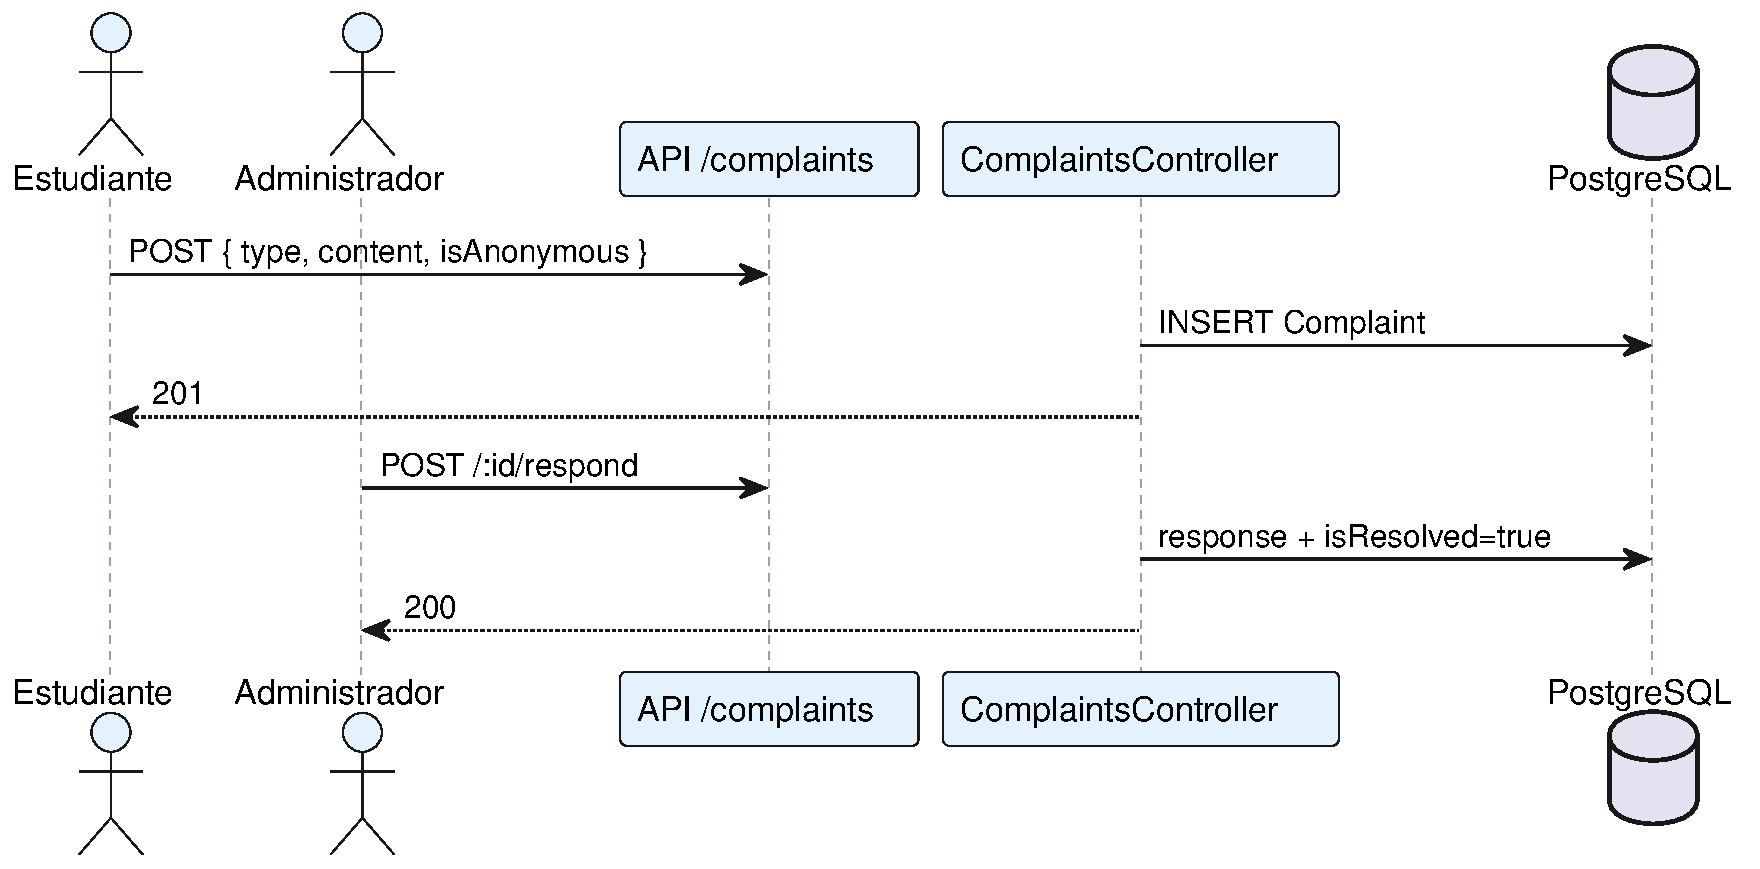
\includegraphics[width=\linewidth,height=0.42\textheight,keepaspectratio]{cu/cu19-seq.pdf}\caption{Diagrama de secuencia --- CU-19}\end{figure}
\begin{figure}[H]\centering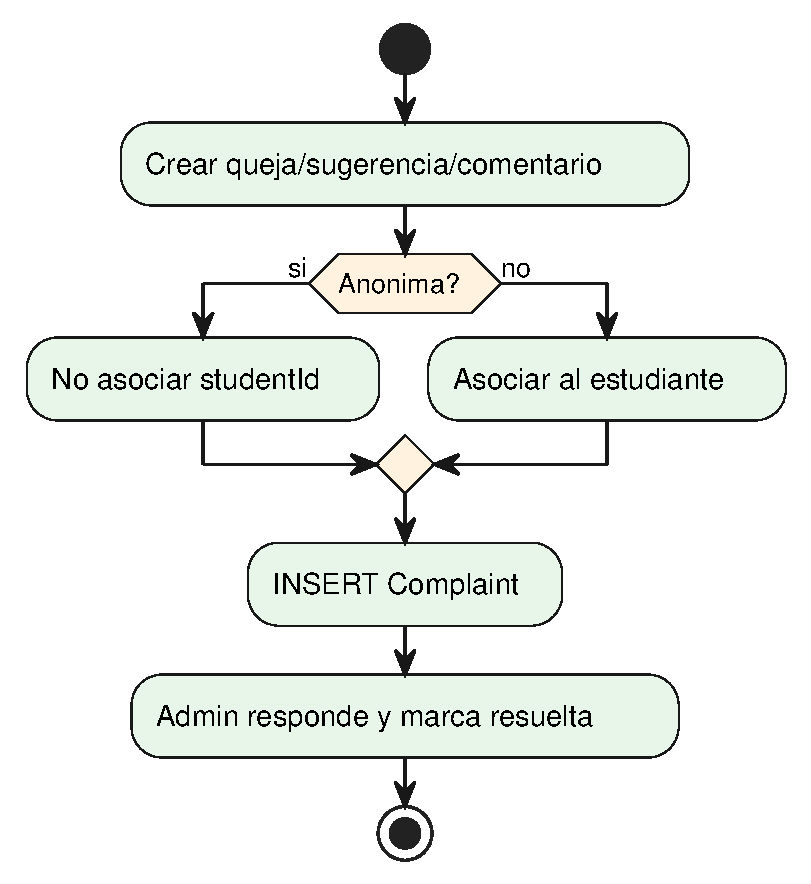
\includegraphics[width=\linewidth,height=0.46\textheight,keepaspectratio]{cu/cu19-act.pdf}\caption{Diagrama de actividades --- CU-19}\end{figure}

\subsection{CU-20 --- Gestionar noticias}

\noindent\textbf{Endpoint(s):} \texttt{GET/POST/PUT/DELETE /api/news}\par\vspace{4pt}

\begin{table}[H]\centering\small
\caption{Ficha del caso de uso CU-20 --- Gestionar noticias}
\begin{tabularx}{\textwidth}{L{0.26\textwidth} X}
\toprule
\textbf{Campo} & \textbf{Descripcion} \\ \midrule
Objetivo del contexto & Permitir al administrador publicar, editar y eliminar noticias visibles para los usuarios. \\ \midrule
Precondiciones & El administrador debe estar autenticado con rol admin. \\ \midrule
Condicion de exito & La noticia se crea, actualiza o desactiva. \\ \midrule
Condicion de fracaso & Datos invalidos o noticia inexistente. \\ \midrule
Actores principales & Administrador, Usuario \\ \midrule
Actores secundarios & Base de datos \\
\bottomrule\end{tabularx}\end{table}
\begin{table}[H]\centering\small
\caption{Flujo principal de CU-20}
\begin{tabularx}{\textwidth}{C{0.10\textwidth} X}
\toprule \textbf{Paso} & \textbf{Accion} \\ \midrule
1 & El administrador selecciona la operacion sobre la noticia. \\
2 & El sistema valida los datos. \\
3 & El sistema crea, actualiza o desactiva (soft delete) la noticia. \\
4 & Los usuarios consultan las noticias activas. \\
\bottomrule\end{tabularx}\end{table}
\begin{table}[H]\centering\small
\caption{Extensiones (flujos alternativos) de CU-20}
\begin{tabularx}{\textwidth}{C{0.10\textwidth} X}
\toprule \textbf{Paso} & \textbf{Accion} \\ \midrule
2.1 & Datos invalidos $\rightarrow$ HTTP 400. \\
3.1 & Noticia inexistente $\rightarrow$ HTTP 404. \\
\bottomrule\end{tabularx}\end{table}
\begin{figure}[H]\centering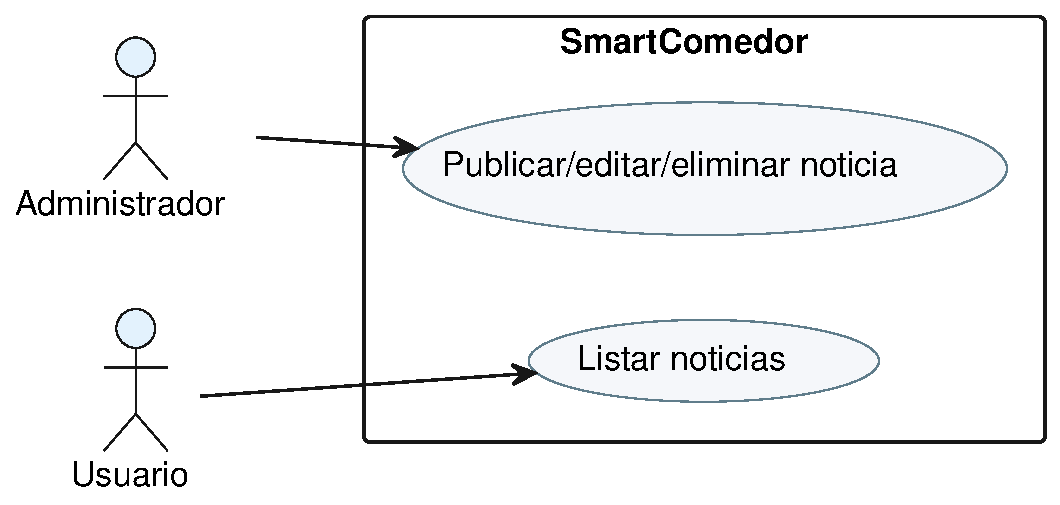
\includegraphics[width=\linewidth,height=0.30\textheight,keepaspectratio]{cu/cu20-uc.pdf}\caption{Diagrama de caso de uso --- CU-20}\end{figure}
\begin{figure}[H]\centering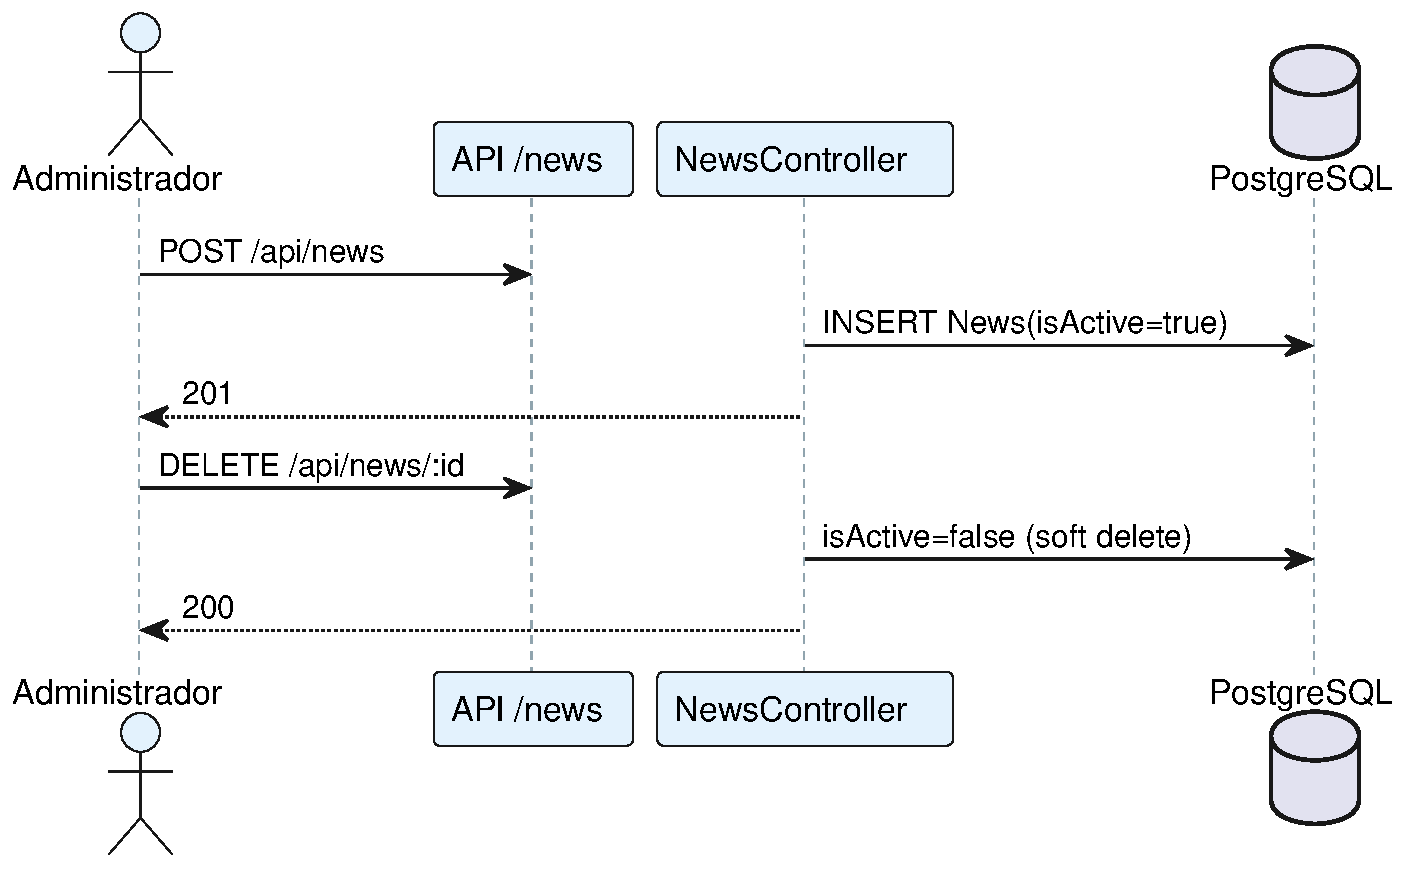
\includegraphics[width=\linewidth,height=0.42\textheight,keepaspectratio]{cu/cu20-seq.pdf}\caption{Diagrama de secuencia --- CU-20}\end{figure}
\begin{figure}[H]\centering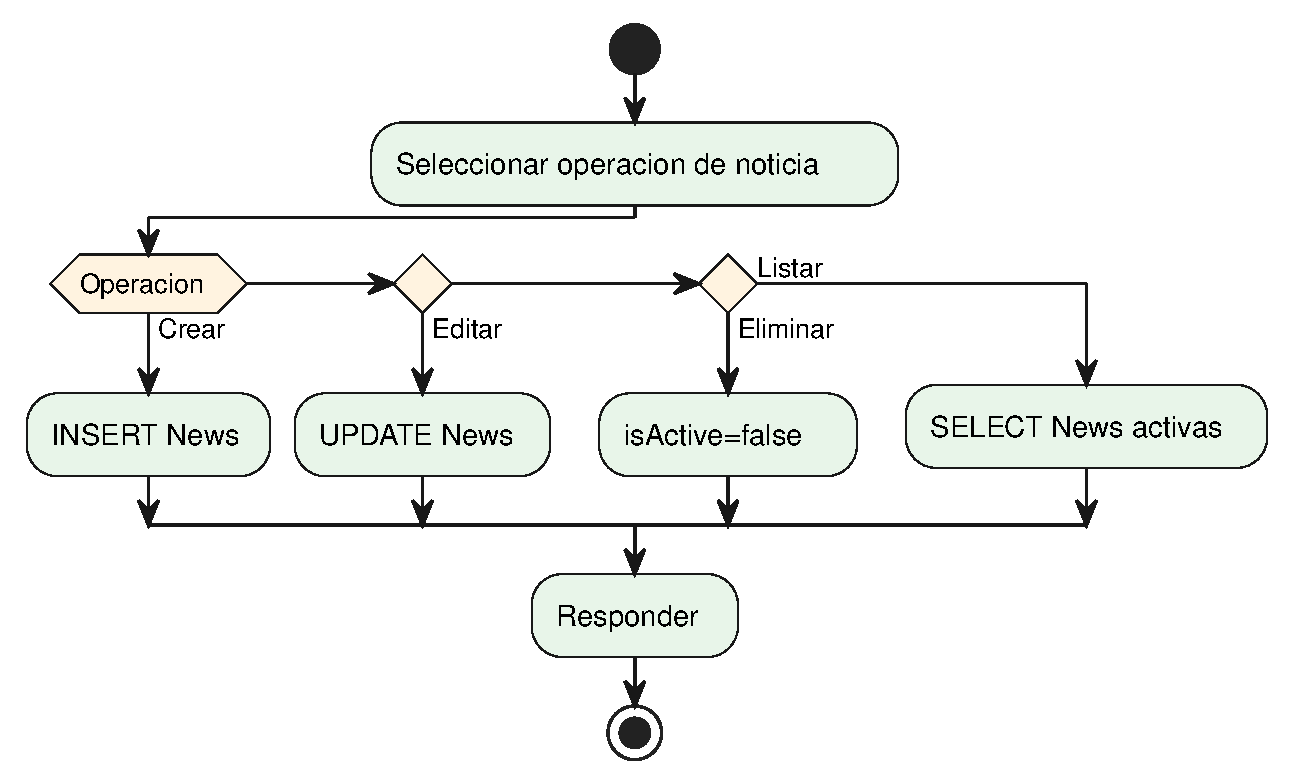
\includegraphics[width=\linewidth,height=0.46\textheight,keepaspectratio]{cu/cu20-act.pdf}\caption{Diagrama de actividades --- CU-20}\end{figure}

\subsection{CU-21 --- Consultar auditoria}

\noindent\textbf{Endpoint(s):} \texttt{GET /api/audit}\par\vspace{4pt}

\begin{table}[H]\centering\small
\caption{Ficha del caso de uso CU-21 --- Consultar auditoria}
\begin{tabularx}{\textwidth}{L{0.26\textwidth} X}
\toprule
\textbf{Campo} & \textbf{Descripcion} \\ \midrule
Objetivo del contexto & Permitir a los perfiles autorizados consultar la bitacora de auditoria del sistema con filtros controlados. \\ \midrule
Precondiciones & El usuario debe tener rol admin o auditor. \\ \midrule
Condicion de exito & Se devuelven los eventos de auditoria paginados. \\ \midrule
Condicion de fracaso & Filtros fuera de la lista blanca. \\ \midrule
Actores principales & Administrador, Auditor externo \\ \midrule
Actores secundarios & Base de datos \\
\bottomrule\end{tabularx}\end{table}
\begin{table}[H]\centering\small
\caption{Flujo principal de CU-21}
\begin{tabularx}{\textwidth}{C{0.10\textwidth} X}
\toprule \textbf{Paso} & \textbf{Accion} \\ \midrule
1 & El usuario ingresa filtros (accion, metodo, fechas). \\
2 & El sistema valida los filtros contra una lista blanca. \\
3 & El sistema consulta audit\_logs con paginacion. \\
4 & El sistema responde 200 con los eventos. \\
\bottomrule\end{tabularx}\end{table}
\begin{table}[H]\centering\small
\caption{Extensiones (flujos alternativos) de CU-21}
\begin{tabularx}{\textwidth}{C{0.10\textwidth} X}
\toprule \textbf{Paso} & \textbf{Accion} \\ \midrule
2.1 & Filtro no permitido $\rightarrow$ HTTP 400. \\
\bottomrule\end{tabularx}\end{table}
\begin{figure}[H]\centering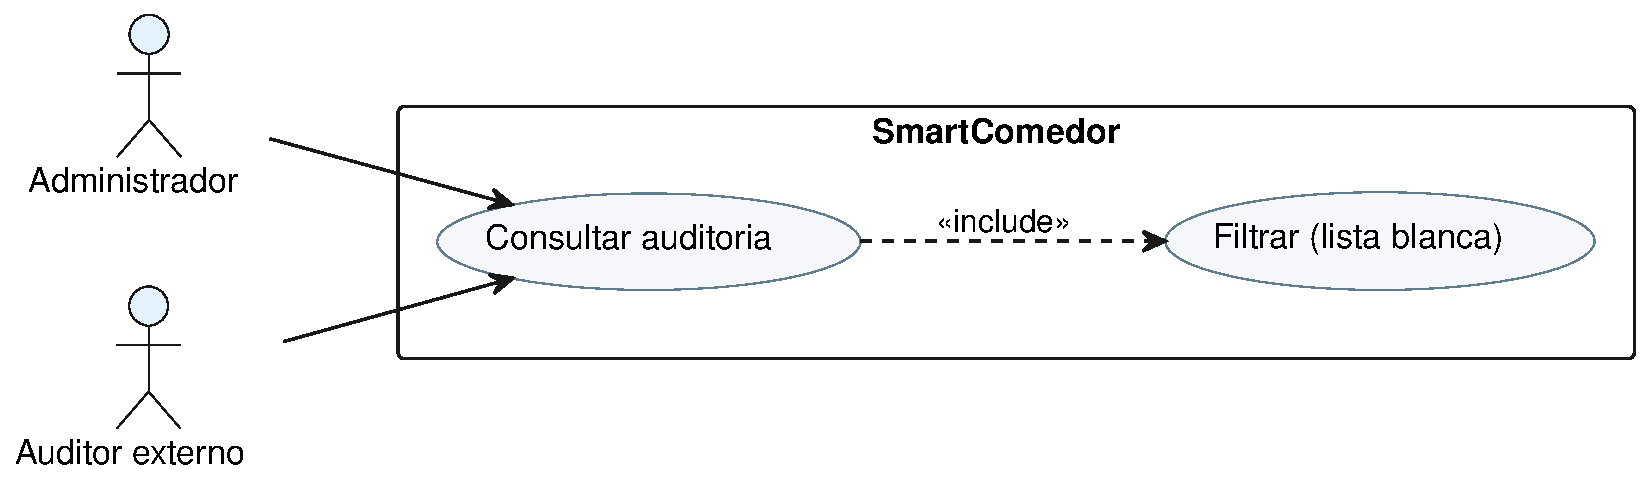
\includegraphics[width=\linewidth,height=0.30\textheight,keepaspectratio]{cu/cu21-uc.pdf}\caption{Diagrama de caso de uso --- CU-21}\end{figure}
\begin{figure}[H]\centering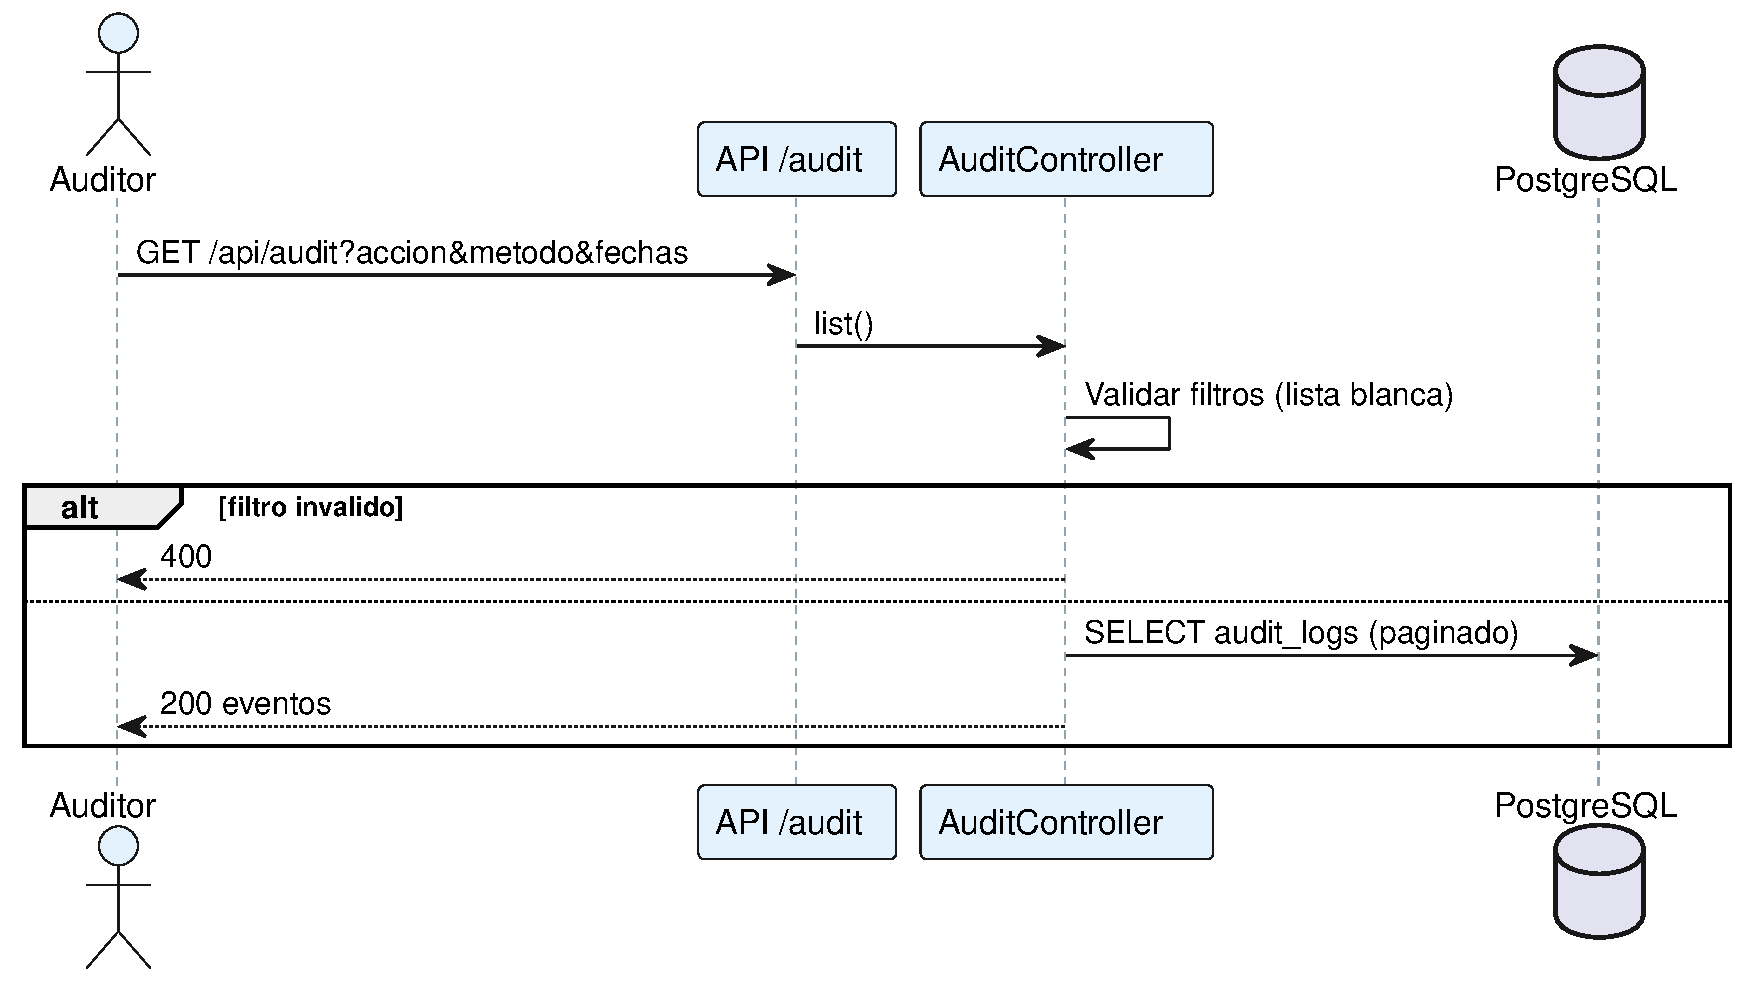
\includegraphics[width=\linewidth,height=0.42\textheight,keepaspectratio]{cu/cu21-seq.pdf}\caption{Diagrama de secuencia --- CU-21}\end{figure}
\begin{figure}[H]\centering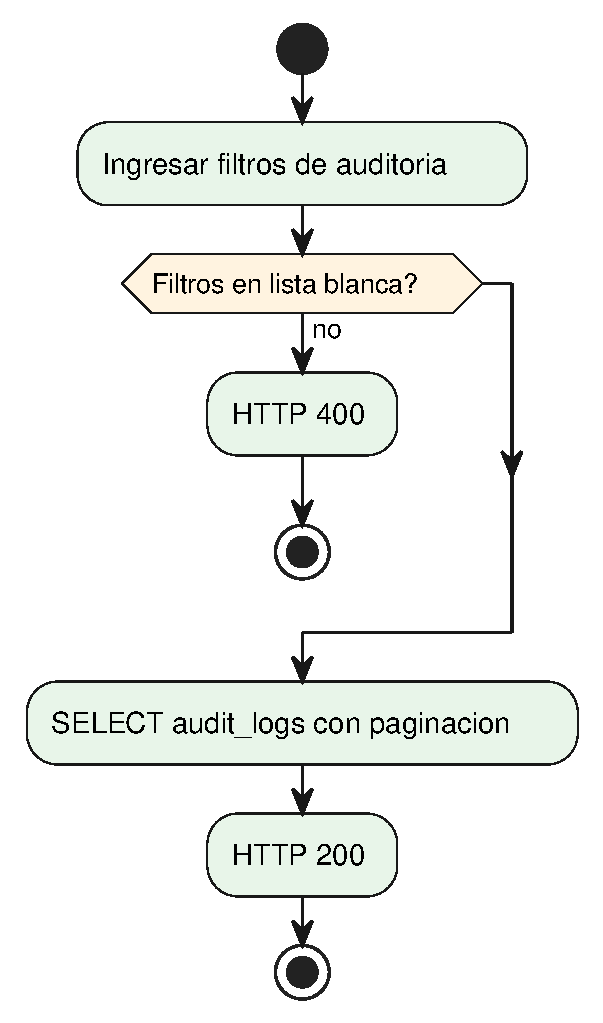
\includegraphics[width=\linewidth,height=0.46\textheight,keepaspectratio]{cu/cu21-act.pdf}\caption{Diagrama de actividades --- CU-21}\end{figure}
